\documentclass[12pt,italian]{report}
\usepackage{tesi}

% DATI STUDENTE e TESI
%\newcommand{\myTitle}{Model Predictive Control con robot mobili autonomi nello scenario di robot racing F1TENTH}
%\newcommand{\myRefereeA}{Matteo Luperto}
%\newcommand{\myRefereeB}{Michele Antonazzi}
%\newcommand{\myName}{\textbf{Vincenzo Siano}}
%\newcommand{\myMat}{Matr.\@ 981734}
%\newcommand{\myYY}{2023-2024}
%\newcommand{\dept}{Corso di Laurea in Informatica}
\university{Università degli Studi di Milano}
\graphicspath{ {images/} }
\unilogo{images/logo.png}
\faculty{Facoltà di Scienze e Tecnologie}
\department{Dipartimento di Informatica\\Giovanni Degli Antoni}
\cdl{Corso di Laurea in Informatica}

%   TITOLO TESI:
\title{Ottimizzazione del Path Tracking con Model Predictive Control per Autonomous Racing in F1TENTH}
\printedtitle{Ottimizzazione del Path Tracking con Model Predictive Control per Autonomous Racing in F1TENTH}

% Questo comando (opzionale) sovrascrive \title per quanto riguarda la copertina
% Può essere usato per stampare caratteri speciali, tenendo i metadati puliti
%\printedtitle{Path Tracking ottimizzato con Model Predictive Control\\per Autonomous Racing nel contesto di F1TENTH}
%\printedtitle{Model Predictive Control\\per Autonomous Racing\\nel contesto di F1TENTH}
%   AUTORE:
\author{Vincenzo Siano}
\matricola{981734}
\typeofthesis{Tesi di Laurea}

%   RELATORE E CORRELATORE:
\relatore{Matteo Luperto}
\correlatore{Michele Antonazzi}
%\correlatore{}

%   LABORATORIO
\aislab

% Esempio di personalizzazione
\lab{Laboratorio di Ricerca}
% \lab[in collaborazione con l']{Azienda Specifica}
\laburl{https://di.unimi.it/it/ricerca/risorse-e-luoghi-della-ricerca/laboratori-di-ricerca}
\lablogo{images/logo}

%   ANNO ACCADEMICO
% \the\year inserisce l'anno corrente
% per specificare manualmente un anno accademico
% NON inserire nel formato 1970-1971, ma
% inserire solo 1970
\academicyear{2023} 

% Package di formato
\usepackage[a4paper]{geometry}		% Formato del foglio
\usepackage[italian]{babel}			% Supporto per l'italiano
\usepackage[utf8]{inputenc}			% Supporto per UTF-8
\usepackage{afterpage, lscape}
%\usepackage[a-1a]{pdfx}			    % File conforme allo standard PDF-A (obbligatorio per la consegna)

% Package per la grafica
\usepackage{graphicx}				% Funzioni avanzate per le immagini
\usepackage{float}
\usepackage{subcaption}

\usepackage{setspace}
%\usepackage{amsmath}
%\usepackage{amssymb}
\usepackage{bm}
\usepackage{algorithm}              % Scrittura di algoritmi
\usepackage{algpseudocodex}         % Scrittura di algoritmi
\algrenewcommand\algorithmicrequire{\textbf{Input:}}
\usepackage{listings}				% Scrittura di codice
\usepackage{minted}                 % Scrittura di codice
\usemintedstyle{emacs}
\usepackage{xcolor}

\definecolor{codegreen}{rgb}{0,0.6,0}
\definecolor{codegray}{rgb}{0.5,0.5,0.5}
\definecolor{codepurple}{rgb}{0.58,0,0.82}
\definecolor{backcolour}{rgb}{0.96,0.96,0.96}

\lstdefinestyle{mystyle}{
    backgroundcolor=\color{backcolour},   
    commentstyle=\color{codegreen},
    keywordstyle=\color{magenta},
    numberstyle=\tiny\color{codegray},
    stringstyle=\color{codepurple},
    basicstyle=\ttfamily\footnotesize,
    breakatwhitespace=false,         
    breaklines=true,                 
    captionpos=b,                    
    keepspaces=true,                 
    numbers=left,                    
    numbersep=5pt,                  
    showspaces=false,                
    showstringspaces=false,
    showtabs=false,                  
    tabsize=2
}

%\lstset{style=mystyle}

% color def
\usepackage{color}
\definecolor{darkred}{rgb}{0.6,0.0,0.0}
\definecolor{darkgreen}{rgb}{0,0.50,0}
\definecolor{lightblue}{rgb}{0.0,0.42,0.91}
\definecolor{orange}{rgb}{0.84,0.34,0}
\definecolor{grass}{rgb}{0,0.65,0.03}
\definecolor{pink}{rgb}{0.97,0.15,0.45}


% General Setting of listings
\lstset{
  aboveskip=1em,
  breaklines=true,
  abovecaptionskip=-6pt,
  captionpos=b,
  escapeinside={\%*}{*)},
  frame=single,
  numbers=left,
  numbersep=10pt,
  numberstyle=\tiny,
}
% 0. Basic Color Theme
\lstdefinestyle{colored}{ %
  basicstyle=\ttfamily,
  backgroundcolor=\color{white},
  commentstyle=\color{green}\itshape,
  keywordstyle=\color{blue}\bfseries\itshape,
  stringstyle=\color{red},
}
% 1. General Python Keywords List
\lstdefinelanguage{PythonPlus}[]{Python}{
  morekeywords=[1]{,as,assert,nonlocal,with,yield,self,@,True,False,None,} % Python builtin
  morekeywords=[2]{,__init__,__add__,__mul__,__div__,__sub__,__call__,__getitem__,__setitem__,__eq__,__ne__,__nonzero__,__rmul__,__radd__,__repr__,__str__,__get__,__truediv__,__pow__,__name__,__future__,__all__,}, % magic methods
  morekeywords=[3]{,object,type,isinstance,copy,deepcopy,zip,enumerate,reversed,list,set,len,dict,tuple,range,xrange,append,execfile,real,imag,reduce,str,repr,}, % common functions
  morekeywords=[4]{,Exception,NameError,IndexError,SyntaxError,TypeError,ValueError,OverflowError,ZeroDivisionError,}, % errors
  morekeywords=[5]{,ode,fsolve,sqrt,exp,sin,cos,arctan,arctan2,arccos,pi, array,norm,solve,dot,arange,isscalar,max,sum,flatten,shape,reshape,find,any,all,abs,plot,linspace,legend,quad,polyval,polyfit,hstack,concatenate,vstack,column_stack,empty,zeros,ones,rand,vander,grid,pcolor,eig,eigs,eigvals,svd,qr,tan,det,logspace,roll,min,mean,cumsum,cumprod,diff,quad_form,vec,block_diag,vectorize,lstsq,cla,eye,xlabel,ylabel,squeeze,}, % numpy / math
}
% 2. New Language based on Python
\lstdefinelanguage{PyBrIM}[]{PythonPlus}{
  emph={d,E,a,Fc28,Fy,Fu,D,des,supplier,Material,Rectangle,PyElmt},
}
% 3. Extended theme
\lstdefinestyle{colorEX}{
  basicstyle=\ttfamily\footnotesize,
  backgroundcolor=\color{white},
  commentstyle=\color{darkgreen}\slshape,
  keywordstyle=\color{blue}\bfseries\itshape,
  keywordstyle=[2]\color{blue}\bfseries,
  keywordstyle=[3]\color{grass},
  keywordstyle=[4]\color{red},
  keywordstyle=[5]\color{orange},
  stringstyle=\color{darkred},
  emphstyle=\color{pink}\underbar,
}

\lstset{style=colorEX}

% Package Biblatex
\usepackage{csquotes}
\usepackage[backend=biber,style=numeric,sorting=none,maxbibnames=50]{biblatex}
\addbibresource{bibliography.bib}

% Package ipertesto
\usepackage{url}					% Visualizza e rendere interattii gli URL
\usepackage{hyperref}	            % Rende interattivi i collegamenti interni
\hypersetup{
    %hidelinks % Nasconde i riquardi colorati brutti, si può cambiare con hyperref anche (da vedere)
    bookmarksopen=true,
    %colorlinks=true,
    %citecolor=[RGB]{12, 133, 11},
    %linkcolor=[RGB]{0, 32, 69},
    %urlcolor=[RGB]{0, 73, 158},
}

%\graphicspath{ {images/} }


%\renewcommand{\baselinestretch}{1.3} %\linespread{1.3}

%   INDICI
% elenco delle figure (facoltativo)
% \figurespagetrue
% elenco delle tabelle (facoltativo)
% \tablespagetrue
% prefazioni nell'indice (facoltativo)
%\prefaceintoctrue
% indice nell'indice (facoltativo)
\tocintoctrue

% --- FINE PREAMBOLO ----------------------------------------------------------
\begin{document}
\makefrontpage
\newgeometry{top=2cm,bottom=2cm}
\beforepreface

% 
%			PREFAZIONE (facoltativa)
%

% \prefacesection{Prefazione}
% Le prefazioni non sono molto comuni, tuttavia a volte capita che qualcuno voglia dire qualcosa che esuli dal lavoro in sé (come un meta-commento sull'elaborato), o voglia fornire informazioni riguardanti l'eventuale progetto entro cui la tesi si colloca (in questo caso è probabile che sia il relatore a scrivere questa parte).

%
%			Creazione automatica dell'indice
%

\afterpreface
\restoregeometry

\chapter{Introduzione}
\label{chap:chap1}
% OTTIMIZZAZIONE DEL PATH TRACKING CON MODEL PREDICTIVE CONTROL PER AUTONOMOUS RACING NEL CONTESTO DI F1TENTH
% Presentare il lavoro svolto e gli obiettivi da raggiungere
Nell'ultimo decennio il settore della guida autonoma ha fatto grandi progressi grazie
all'introduzione di nuovi algoritmi e tecniche avanzate nel campo della robotica e 
dell'intelligenza artificiale. L'\textit{autonomous driving} rappresenta una sfida
tecnologica molto complessa poiché è caratterizzata da diversi ambiti di ricerca, quali 
percezione, pianificazione e controllo.
In aggiunta alle più classiche applicazioni di guida autonoma, come il trasporto
pubblico urbano e le automobili con funzionalità di guida assistita o totalmente autonoma,
un settore altamente competitivo che sta attirando sempre più attenzione è quello 
dell'\textit{autonomous racing}. Le auto da corsa possono essere veicoli reali -- come 
una vettura di \textit{Formula 1} -- o veicoli a scala ridotta -- ad esempio scala 1:10 per \textit{F1TENTH}.
Proprio comunità come quella di \textit{F1TENTH} stanno raggiungendo ottimi risultati grazie a delle vere e
proprie competizioni, che permettono di far gareggiare ingegneri e ricercatori provenienti
da tutto il mondo con veicoli autonomi in condizioni estreme, mettendo alla prova le 
prestazioni delle proprie soluzioni in ambienti a velocità elevate, come dei circuiti.
I partecipanti possono così affrontare le sfide del controllo più estreme in un 
ambiente controllato, riflettendo però le dinamiche del mondo reale.

A differenza della guida su strada, lo scopo è quello di guidare in sicurezza nel modo
più veloce ed efficiente, riducendo i tempi di completamento su piste competitive. 
In questo contesto, vi sono dunque due sfide cruciali: la pianificazione della traiettoria e sistemi di controllo robusti e accurati, in grado di gestire variazioni improvvise.
Inoltre, il controllo del veicolo ha il compito di ottimizzare il percorso seguito e di minimizzare gli errori di traiettoria. 
%Metodi reattivi come \textit{Pure Pursuit} e \textit{PID Controller} sono stati ampiamente usati fino a un certo punto, ma di recente metodi più sofisticati, come il Model Predictive Control (MPC), hanno mostrato un enorme potenziale.

L'obiettivo del lavoro di tesi è sviluppare e analizzare l'efficacia di 
\textit{Model Predictive Control (MPC)}, un metodo di controllo avanzato per 
l'ottimizzazione dell'attività di \textit{path tracking}, applicata in un
contesto di \textit{autonomous racing} su veicoli in scala 1:10 per la piattaforma
\textit{F1TENTH}.
Attraverso l'implementazione dell'algoritmo e la simulazione su diversi tracciati di 
\textit{Formula 1}, si confrontano le prestazioni di \textit{MPC} con quelle di 
\textit{Pure Pursuit}, un altro algoritmo di controllo più semplice basato su 
\textit{metodi reattivi}, secondo diverse metriche individuate.

Il lavoro è stato suddiviso nelle seguenti fasi:
\begin{description}
\item[Capitolo 1: Introduzione] Si fornisce una panoramica di \textit{F1TENTH} e del 
contesto dell'\textit{autonomous racing}. In seguito, si introducono i concetti 
chiave di \textit{ROS}, alla base di tutta l'implementazione del progetto.
\item[Capitolo 2: Metodi reattivi per il controllo] Si discutono i metodi di controllo 
reattivi, come il \textit{PID Controller}, individuando vantaggi e limitazioni di queste
soluzioni per il contesto trattato.
\item[Capitolo 3: Model Predictive Control] Si descrive l'algoritmo oggetto di questa 
tesi, trattandone la struttura, l'\textit{orizzonte}, il modello utilizzato e formulando
il problema di controllo ottimale (obiettivo e vincoli). 
Si discute poi di discretizzazione, linearizzazione e dei vantaggi e svantaggi di questo metodo.
\item[Capitolo 4: Implementazione] Vengono presentati i circuiti utilizzati per mettere alla
prova \textit{MPC} e le sue diverse configurazioni di guida. Dopodiché, si descrive il 
risolutore utilizzato e si discute il codice degli obiettivi e dei vincoli. 
Infine, si approfondisce la fase di \textit{tuning} delle matrici di pesi, fondamentali per l'obiettivo.
\item[Capitolo 5: Analisi dei risultati] Si analizzano i risultati dei profili di \textit{MPC} 
su entrambe le piste, confrontandoli tra loro e con il \textit{Pure Pursuit}.
\item[Capitolo 6: Conclusioni] Si riassumono i principali risultati ottenuti e si
menzionano possibili sviluppi futuri.
\end{description}

%\begin{description}
\section{F1TENTH}
%\lipsum[2]
\textit{F1TENTH} è una comunità internazionale di ricercatori, ingegneri, sviluppatori e appassionati di sistemi autonomi che ogni anno organizza una serie di gare
tra auto autonome da corsa in scala \textit{1:10}, nelle quali squadre provenienti 
da tutto il mondo si riuniscono per competere~\cite{f1tenth}.
Fondata nel 2016 dall'\textit{University of Pennsylvania}, comprende ora diverse università 
provenienti da tutto il mondo, le quali hanno incluso \textit{F1TENTH} nei programmi dei propri 
corsi di laurea, portando a un ulteriore sviluppo della comunità globale.
%\hyperlink{https://f1tenth.org/learn.html}{primo}

\begin{figure}[H]
    \centering
    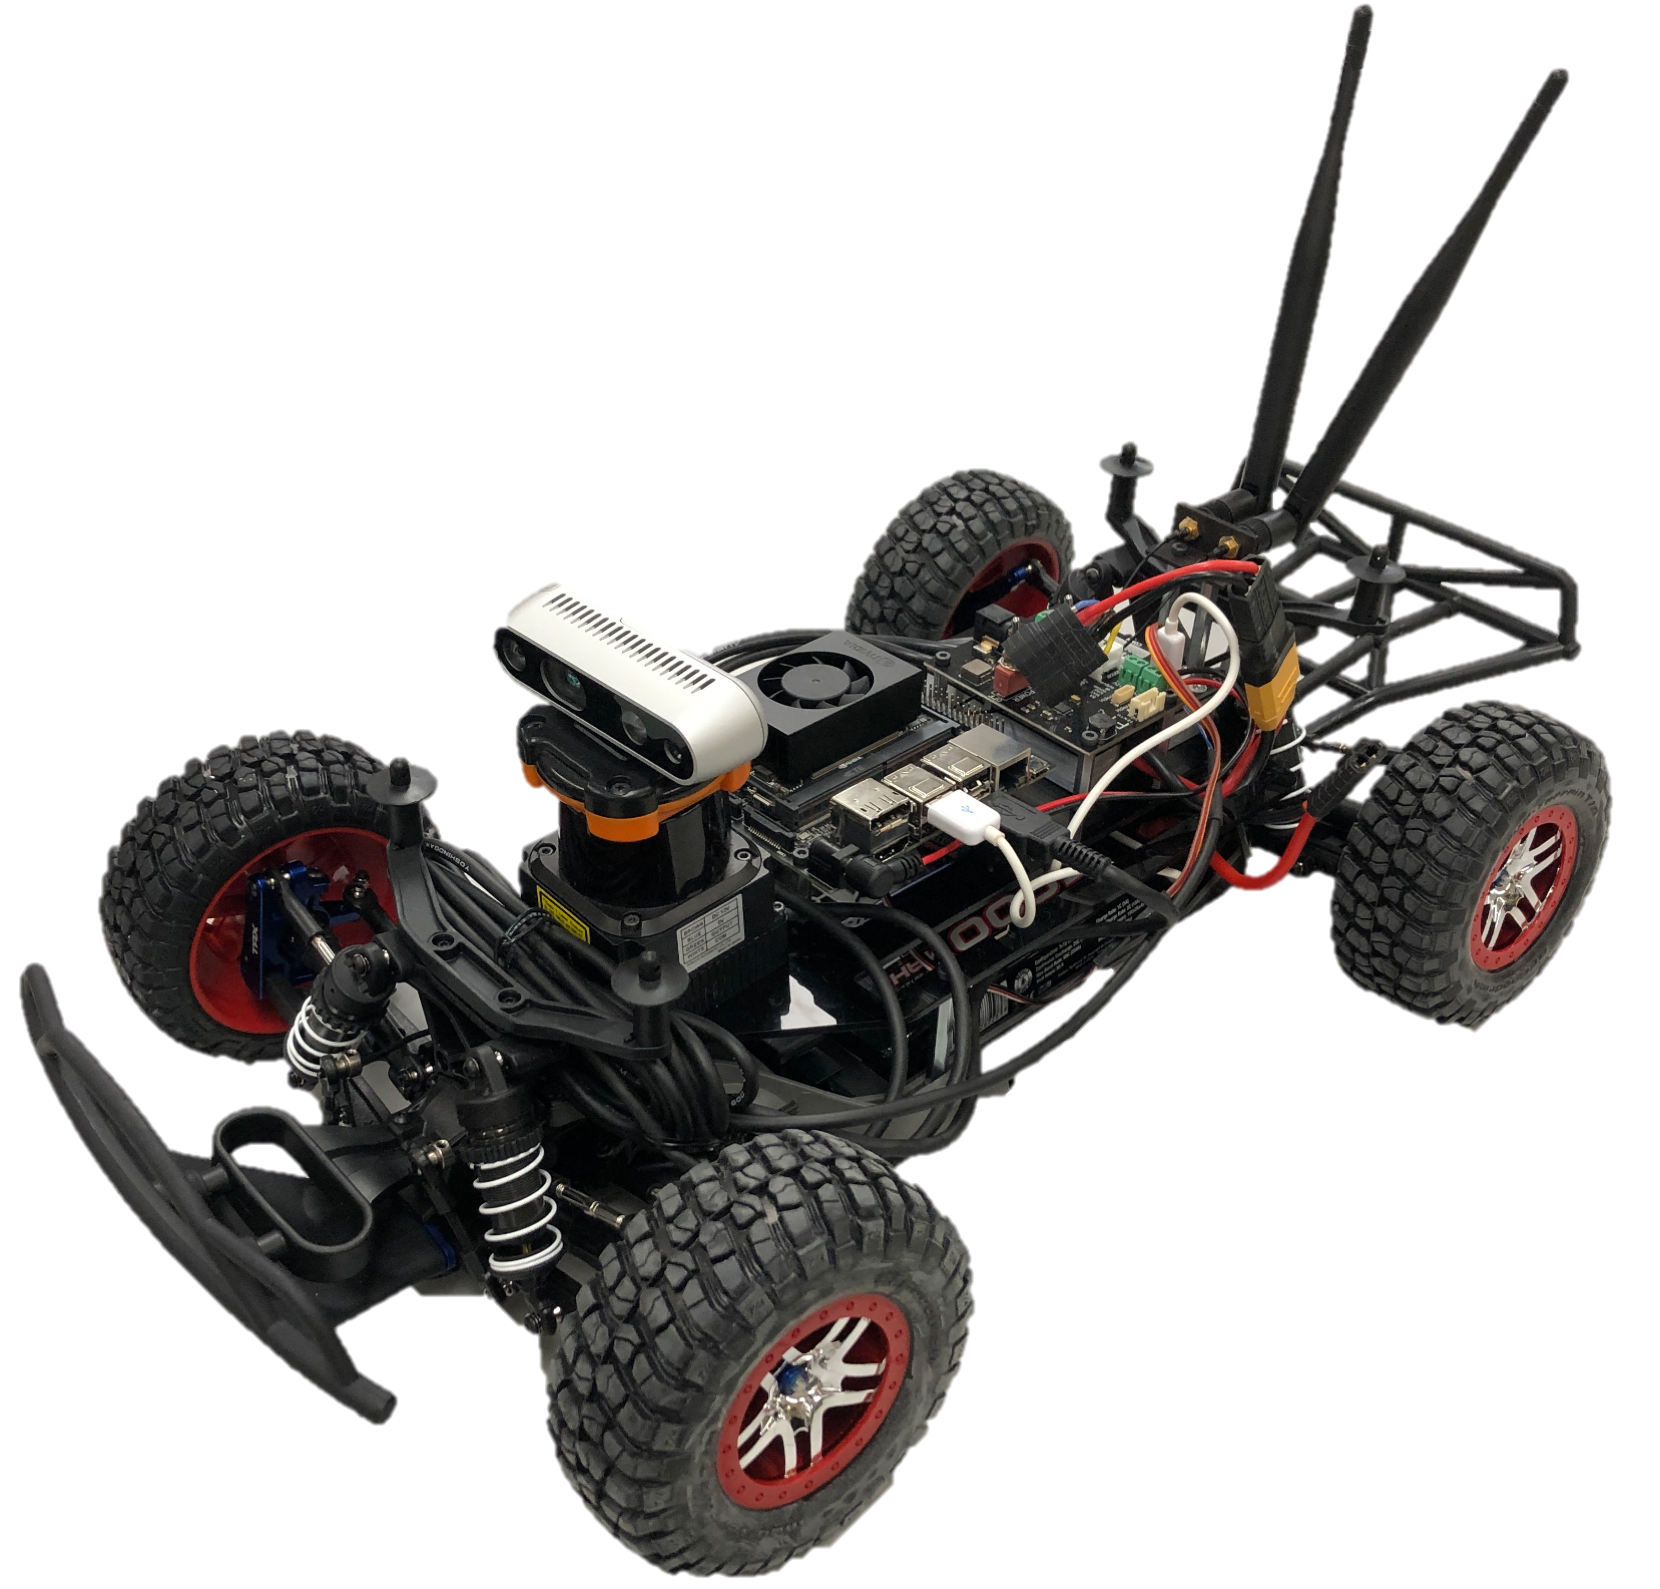
\includegraphics[scale=0.1]{images/F110_car.png}
    \caption{Robot mobile di \textit{F1TENTH} in scala 1:10~\cite{f1tenth}.}
    \label{fig:fig1} % etichetta utilizzata per riferisi all'immagine
\end{figure}

%Oltre alle competizioni, i fondatori hanno organizzato dei corsi gratuiti che insegnano
%i fondamenti della guida autonoma, introducendo gli studenti all'hardware, al software
%e agli algoritmi coinvolti nella costruzione e nello sviluppo di un'auto a guida autonoma. 
%Questi corsi incentivano 
La piattaforma di sviluppo di \textit{F1TENTH} incentiva lo studio e la ricerca nelle 
discipline della guida autonoma, della robotica e dell'intelligenza artificiale; inoltre, essa 
permette di andare a sviluppare anche le capacità analitiche necessarie per ragionare su 
situazioni etiche nella fase di progettazione dei propri veicoli autonomi.

L'obiettivo degli organizzatori consiste quindi nel fornire le basi sulle più
recenti tecnologie implementate e testate sulle auto a guida autonoma e, più in generale, sui sistemi mobili autonomi.
\begin{figure}[H]
    \centering
    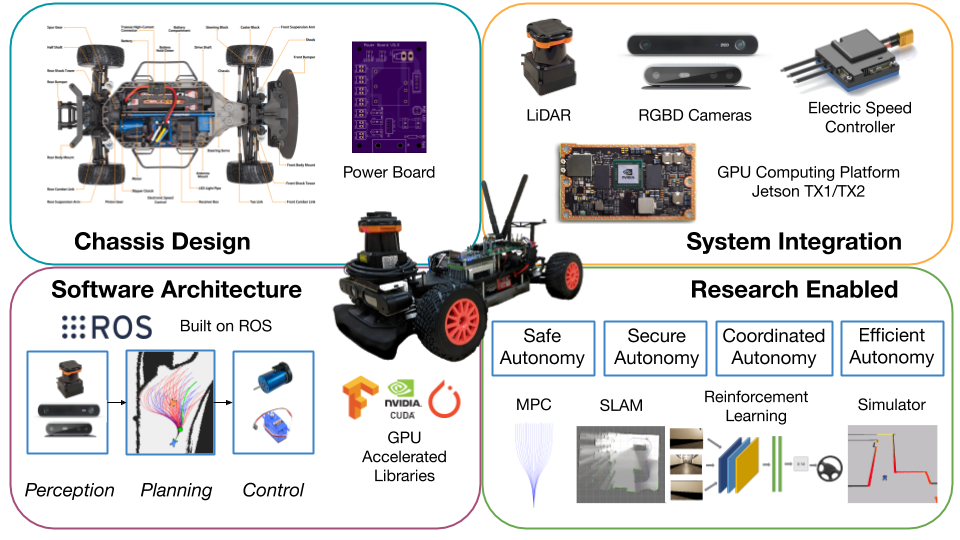
\includegraphics[width=\textwidth]{images/F110_architecture.png}
    \caption{Stack architetturale di \textit{F1TENTH}~\cite{learnf1tenth}.}
    \label{fig:fig2} % etichetta utilizzata per riferisi all'immagine
\end{figure}
\noindent In primo luogo, è stato effettuato uno studio preliminare della piattaforma F1TENTH e dei concetti 
fondamentali della guida autonoma. Essi comprendono le seguenti macro-aree tematiche:
\begin{itemize}
    \item Infrastruttura di \textit{ROS 2} e il simulatore \textit{F1TENTH Gym};
    \item Dinamica del veicolo e \textit{metodi reattivi} -- Comprende la modellazione e la 
    simulazione della dinamica del veicolo, i metodi
    di navigazione reattiva, come l'algoritmo 
    \textit{PID} applicato al \textit{Wall Following} e l'algoritmo \textit{Follow the Gap} per evitare gli ostacoli.
    \item \textit{Mapping} e \textit{Localization} -- Concetti come la stima dello stato, la 
    modellazione dell'ambiente, le tecniche basate su filtri per la localizzazione del robot e la tecnica \textit{SLAM}.
    \item \textit{Control} e \textit{Planning} -- Tematiche fondamentali per la progettazione di 
    veicoli a guida autonoma, come il \textit{path tracking} con \textit{Pure Pursuit}
    e gli algoritmi di pianificazione del movimento di un robot, come \textit{RRT}, 
    altri metodi basati su \textit{spline} o \textit{clotoidi} e altri tipi di \textit{planner}.
\end{itemize}
Inoltre, durante questa fase iniziale sono stati implementati, mediante
\textit{Python} e le relative librerie per ROS 2, i seguenti algoritmi:
\begin{enumerate}
    \item \textit{Frenata di emergenza automatica}: si calcola il tempo istantaneo alla
    collisione (\textit{iTTC}) grazie al messaggio \verb|LaserScan| nel simulatore, al cui 
    interno è presente un array che contiene tutte le misurazioni del LiDAR.
    \item \textit{Wall Following}: si è implementato un \textit{controller PID} per 
    far correre l'auto parallelamente alle pareti di un corridoio ad una distanza fissa;
    \item \textit{Follow the Gap}: si tratta di un algoritmo \textit{reattivo}
    per evitare gli ostacoli che permette al robot di percorrere più giri all'interno della mappa utilizzata;
    \item \textit{Pure Pursuit}: è stato utilizzato \textit{SLAM} per effettuare il \textit{mapping}
    e, al contempo, la localizzazione del veicolo. Il \textit{mapping} è il processo di 
    creazione di una rappresentazione dell'ambiente circostante, mentre la \textit{localizzazione} 
    consiste nel determinare la posizione dell'auto rispetto alla mappa. Invece, per ottenere la 
    localizzazione a partire dalla mappa generata, è stato impiegato un \textit{Particle Filter}. 
    È stato così possibile implementare l'algoritmo \textit{Pure Pursuit}, nel quale viene calcolata 
    iterativamente la curvatura dell'arco da seguire. Questo metodo, infatti, permette di seguire una 
    traiettoria composta da più punti (\textit{waypoint}).
    \item \textit{Motion Planning}: è stata realizzata una struttura per il controllo delle 
    collisioni del veicolo, detta \textit{occupancy grid}. In seguito, è stato implementato 
    l'algoritmo \textit{RRT*} come \textit{local planner} e si è utilizzato \textit{Pure Pursuit}
    come controller.
\end{enumerate}
%Una volta realizzati i laboratori e acquisite le basi necessarie per tutto ciò che riguarda la guida autonoma, si è concentrato lo studio sull'implementazione del Model Predictive Control, che rappresenta l'argomento principale del lavoro di tesi, spiegato nel capitolo 
\section{ROS 2}
Il lavoro oggetto di questa tesi è sviluppato a partire da \textit{Robot Operating System (ROS)}, che consiste in un insieme di librerie software e strumenti
per creare applicazioni robotiche~\cite{doi:10.1126/scirobotics.abm6074}. 
Nato nel 2007, il progetto ha visto numerosi cambiamenti, tra cui il passaggio da
ROS 1 a ROS 2.
Contrariamente a come si potrebbe pensare dal nome, \textit{ROS} non è un sistema 
operativo, bensì si tratta di un \textit{middleware} basato su un meccanismo 
di pubblicazione e sottoscrizione anonimo che consente lo scambio di 
messaggi tra diversi processi.
Un \textit{middleware} è un software che si trova a metà tra un sistema operativo e le
applicazioni in esecuzione al suo interno e permette la comunicazione e la gestione
dei dati per applicazioni distribuite~\cite{middleware}.

Si tratta di un progetto \textit{open source} supportato da una grande comunità di
ricercatori nell'ambito della robotica, i quali effettuano rilasci per più distribuzioni \textit{ROS}. 
Alcune di queste sono dotate di supporto a lungo termine, dunque sono più stabili 
e vengono sottoposte a test approfonditi; rientra in questa categoria \textit{ROS 2 Humble}, 
quella usata per questo lavoro.

\textit{ROS 2} fornisce tutte le funzionalità necessarie per la realizzazione di applicazioni robotiche, 
permettendo dunque di risparmiare più tempo e risorse per sviluppo vero e proprio, una 
caratteristica cruciale, soprattutto, in un contesto lavorativo.
Nello specifico, sono supporti due linguaggi di programmazione: \textit{Python} e \textit{C++}, in base alle proprie conoscenze e/o esigenze.
In questa tesi si è scelto di utilizzare il primo per ogni fase implementativa, come si può
notare al Capitolo \ref{chap:chap4}. Nelle prossime sottosezioni si discute invece 
dei concetti alla base di ROS 2.

\subsection{Nodi}
Un \textit{nodo} rappresenta una singola unità logica che svolge una specifica 
funzione all’interno del processo di esecuzione di un robot. 
Ogni nodo in \textit{ROS} può inviare e ricevere dati da altri nodi tramite 
\textit{topic}, servizi e azioni~\cite{rosdocs}. I nodi possono:
\begin{itemize}
    \item pubblicare su \textit{topic} specifici per fornire dati ad altri nodi;
    \item sottoscriversi per ottenere dati da altri nodi;
    \item agire come un client di servizio per far sì che un altro nodo esegua un 
    calcolo per loro, o come un server di servizio per fornire funzionalità ad altri 
    nodi;
    \item analogamente al servizio, agire come action client/server, per calcoli di 
    lunga durata.
    \item fornire \textit{parametri} per modificare il comportamento 
    durante il runtime.
\end{itemize}

\subsection{Topic}
Un \textit{topic} rappresenta il mezzo di comunicazione tramite cui i nodi si 
scambiano i \textit{messaggi} e risulta particolarmente indicato per flussi di dati 
continui, come quelli dei sensori, lo stato del robot e altre informazioni.

I \textit{messaggi} rappresentano il mezzo con cui un nodo invia dati sulla rete
ad altri nodi, senza alcuna risposta prevista. Questi sono descritti e definiti nei file 
\verb|.msg| nella directory \verb|msg/| di un pacchetto \textit{ROS} e sono composti da 
campi e costanti.

Un \textit{topic} è dunque un sistema di pubblicazione/sottoscrizione \textit{fortemente tipizzato}.
Entrando nello specifico, nel sistema dei topic sono presenti produttori di dati (detti 
\textit{``publishers''}) e consumatori di dati (detti \textit{``subscribers''}). Queste due entità 
sanno come mettersi in contatto tra loro proprio grazie al concetto stesso di \textit{topic}, 
identificato da un nome comune per far sì che le entità possano ``vedersi''.
Quando i dati vengono pubblicati nel \textit{topic} da uno qualsiasi dei \textit{publishers}, 
tutti i \textit{subscribers} attivi nel sistema riceveranno i dati.

Questa struttura ricorda molto il concetto di \textit{bus} nell'informatica, poiché assomiglia 
proprio a quello presente nei dispositivi hardware.
Un'altra peculiarità di \textit{ROS} è che, di fatto, tutto è \textit{anonimo}: questo implica 
che, quando un \textit{subscriber} riceve un dato, generalmente non sa quale 
\textit{publisher} lo abbia originariamente inviato, anche se lo si può scoprire. 
Il vantaggio di questa architettura è che entrambi i soggetti possono essere scambiati a piacimento, senza influenzare il resto del sistema.

\subsection{Parametri e Launch file}
I \textit{parametri} consistono in una coppia \verb|<chiave:valore>| e sono associati ai singoli nodi, in modo da configurarli all’avvio e durante il runtime, senza quindi
dover modificare continuamente il codice.
I valori iniziali dei parametri possono essere impostati durante l'esecuzione del 
nodo tramite argomenti da riga di comando, file \verb|YAML|, o quando si esegue
il nodo, con l'uso di \textit{launch file}.

Un sistema sviluppato con ROS 2 è tipicamente costituito da molti nodi che eseguono 
processi diversi, eventualmente anche su macchine differenti. 
In particolare, i grandi progetti di robotica coinvolgono spesso più nodi
interconnessi, ognuno dei quali può avere a sua volta numerosi parametri.
Sebbene sia possibile eseguire ciascuno di questi nodi separatamente, l'operazione 
si complica rapidamente.

Il sistema dei \textit{launch file} in \textit{ROS 2} ha lo scopo di automatizzare
l'esecuzione di più nodi attraverso l'uso di un unico comando: \verb|ros2 launch <nome_launch_file.py>|. 
La configurazione del file include quali programmi eseguire e quali argomenti passare; 
in pratica, questi file -- scritti in \textit{Python}, \verb|YAML| o \verb|XML| --
consentono di configurare e avviare contemporaneamente più eseguibili contenenti
dei nodi di \textit{ROS}. Durante lo sviluppo di questa tesi, essi si sono rivelati
fondamentali per l'operazione di \textit{``tuning''} degli algoritmi realizzati, come si può notare nella sottosezione~\ref{subs:tuning}).

\section{Simulatore: F1TENTH Gym}
Il simulatore utilizzato per svolgere tutto il lavoro di tesi è \textit{F1TENTH Gym}, 
l'ambiente ufficiale ideato a fini ricerca, in quanto è necessaria una simulazione 
asincrona e realistica dei veicoli, con la possibilità di avere anche più istanze di veicoli 
(\textit{agenti}) nello stesso ambiente.

Il motore fisico del simulatore favorisce la presenza di programmi estremamente paralleli e, 
soprattutto, permette di avere un'esecuzione rapida.
Si specifica che \textit{F1TENTH Gym} è il simulatore alla base di \textit{F1TENTH Gym ROS}, 
un bridge di comunicazione con \textit{ROS 2} per \textit{F1TENTH Gym}, che dunque 
viene trasformato in una simulazione vera e propria per \textit{ROS 2}, visualizzandola nell'applicativo \verb|RViz|.

\begin{figure}[H]
    \centering
    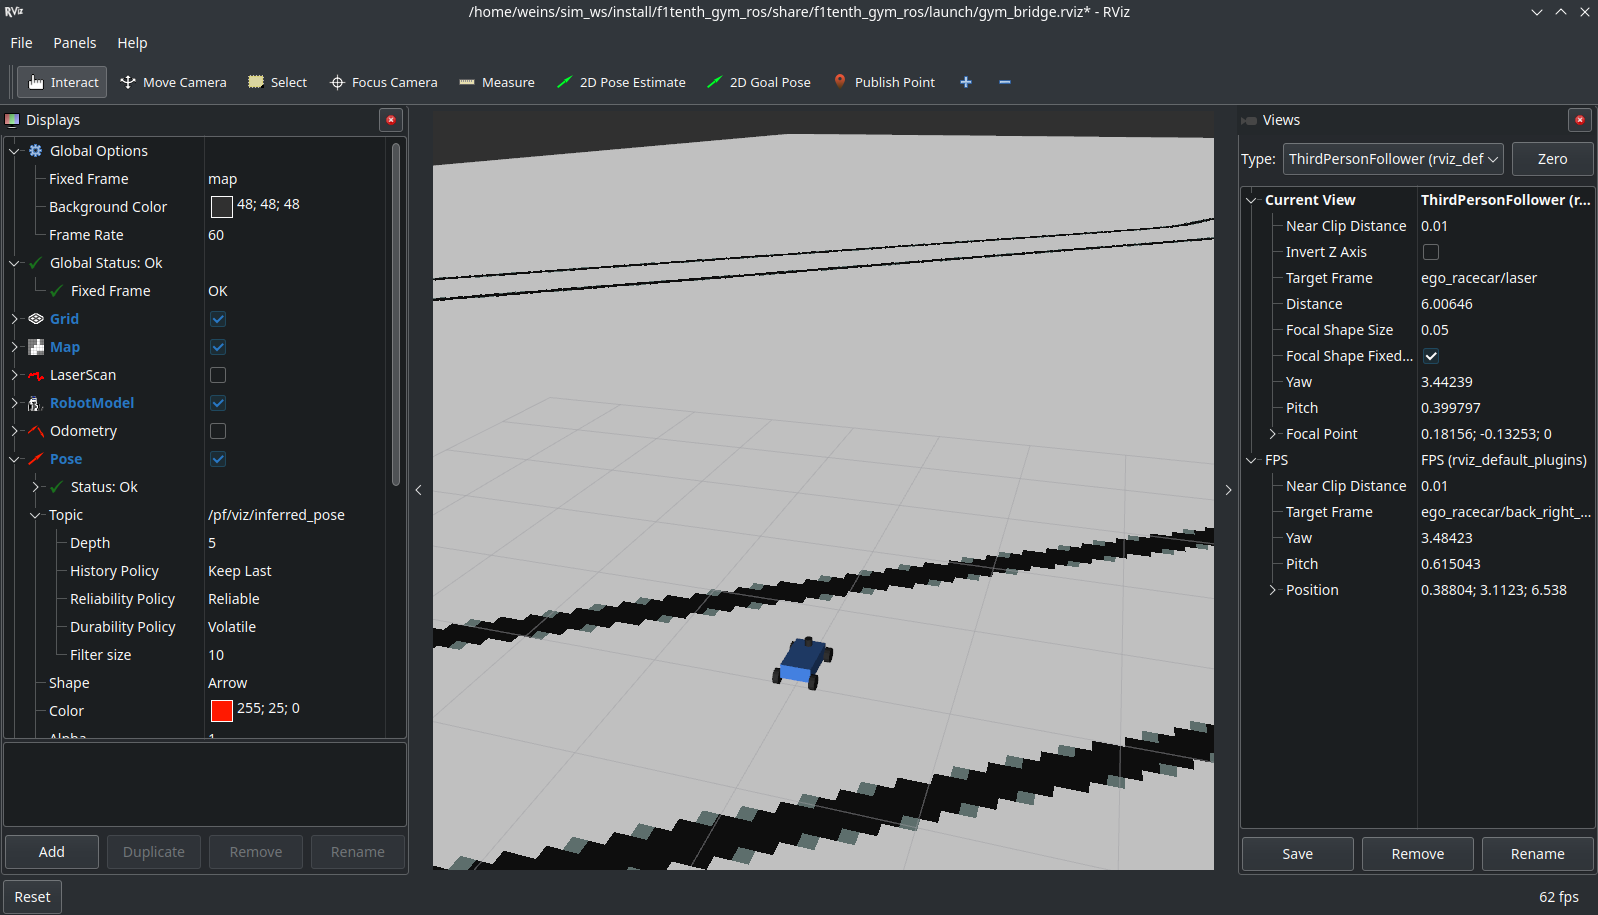
\includegraphics[width=\textwidth]{images/rviz.png}
    \caption{\textit{F1TENTH Gym ROS} con visualizzazione di \textit{RViz}.}
    \label{fig:fig3} % etichetta utilizzata per riferisi all'immagine
\end{figure}

Si specifica che per questo lavoro si è sempre usato un unico agente. Per questa casistica,
i \textit{topic} pubblicati dalla simulazione sono:
\begin{enumerate}
    \item \verb|/scan| -- La scansione laser dell'agente;
    \item \verb|/ego_racecar/odom| -- L'\textit{odometria} dell'agente rappresenta l'uso dei dati provenienti dai sensori di movimento per stimare il cambiamento nel tempo della posizione, dell'orientamento e della velocità.
    \item \verb|/map| -- La mappa dell'ambiente.
\end{enumerate}
Mentre quelli sottoscritti dalla simulazione comprendono:
\begin{enumerate}
    \item \verb|/drive| -- Il comando di guida tramite messaggi \verb|AckermannDriveStamped|.
    \item \verb|/initialpose| -- Permette di reimpostare la posizione dell'agente tramite lo strumento \verb|2D Pose Estimate| di \verb|RViz|.
\end{enumerate}
Anche il nodo \verb|teleop|, relativo al controllo dell'agente con la tastiera, viene incluso come parte della dipendenza del simulatore.

\section{Progettazione dei veicoli a guida autonoma}
La progettazione di veicoli a guida autonoma viene suddivisa in tre macro-aree che
vengono eseguite una dopo l’altra in modo circolare.
% TODO: Spostare sotto la riga di perception

\begin{figure}[h]
    \centering
    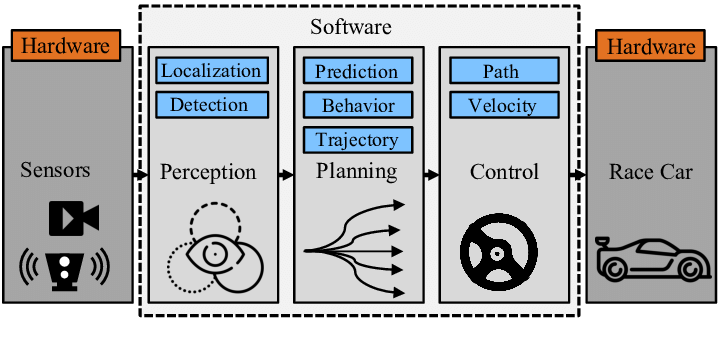
\includegraphics[width=\textwidth]{images/adv_stack.png}
    \caption{Pipeline della guida autonoma~\cite{Betz2022}.}
    \label{fig:fig4} % etichetta utilizzata per riferisi all'immagine
\end{figure}

Ogni area produce degli output utili che vengono passati in input alla 
successiva~\cite{Betz2022}. Dunque, in ordine di esecuzione, il problema è suddiviso in:
\begin{enumerate}
    \item \textit{Perception} -- A partire dai sensori presenti nel robot, costruisce
    un modello dell'ambiente che lo circonda e lo localizza al suo interno.
    \item \textit{Planning} -- Grazie all'output della fase precedente, è in grado
    di determinare il suo stato ed esplorare quelli successivi.
    \item \textit{Control} -- Detto anche \textit{Actuator}, si occupa di generare una 
    sequenza di {input} di sterzata e accelerazione per portare il veicolo allo stato 
    successivo, che è stato generato come output della fase precedente.
\end{enumerate}

Questo ciclo prende anche il nome di \textit{Sense-Plan-Act} e, generalmente, per
garantire una buona performance, lo si vuole completare tra le 20 e 50 volte al secondo.

\subsection{Perception}
La parte di \textit{percezione} comprende la raccolta dei dati dei sensori 
e la successiva elaborazione per avere un \textit{modello} dell'ambiente, proprio
come gli occhi di un guidatore umano.
Di seguito gli obiettivi e le attività svolte da questo modulo applicativo:
\begin{itemize}
    \item \textit{Mapping} -- Si vuole rendere il robot abbastanza intelligente da percepire 
    l’ambiente circostante, così da rilevare ostacoli, altri robot mobili e tutto ciò che lo circonda. 
    \item \textit{Localization} -- Si vuole capire la posizione del robot all’interno
    dell'ambiente. Fondamentalmente, si hanno due tipi di strumenti per ottenere 
    tale conoscenza: le informazioni sull’odometria, fornite dall’\textit{Inertial 
    Measurement Unit (IMU)}, e le informazioni sulle osservazioni,
    fornite dal \textit{LiDAR}.
    \item \textit{Vision} -- Si possono sfruttare metodi classici di visione, come
    \textit{detection} con \textit{OpenCV}, \textit{Visual SLAM}, o metodi basati 
    sul \textit{Deep Learning}, come \textit{Object Detection}. 
    Tuttavia, si specifica che questa tematica non è stata trattata in questo lavoro di tesi.
\end{itemize}
Quando si parla del movimento di un robot mobile bisogna innanzitutto dire che è sempre presente l'incertezza nelle osservazioni; per rappresentare esplicitamente l’incertezza si usa la probabilità, che è alla base dei metodi più comuni per eseguire la localizzazione~\cite{f1tenthcoursel07}, che sono:
\begin{enumerate}
    \item \textit{Bayes Filter}: viene solitamente utilizzato esclusivamente per i casi 
    discreti, cioè con valore finito per lo stato. L’idea alla base è quella di stimare una 
    densità di probabilità nello spazio degli stati condizionata dai dati (percettivi e odometrici).
    \item \textit{Kalman Filter}: algoritmo ricorsivo che utilizza una combinazione di 
    predizioni e misurazioni per stimare lo stato di un sistema nel tempo. Utilizza un metodo 
    basato sui campioni per rappresentare una determinata distribuzione.
    \item \textit{Particle Filter}: chiamato anche \textit{Adaptive Monte Carlo}, si basa su un 
    campionamento pesato e casuale. Si tratta di un \textit{Bayes Filter} ricorsivo,
    simile al \textit{Kalman Filter}, ma ne ``rilassa'' alcune assunzioni. Ogni particella è 
    un’ipotesi di posizione e, invece di campionare ogni volta, ciascun campione viene 
    propagato con il modello di movimento per ottenere i campioni nell’iterazione successiva.
\end{enumerate}

Per il problema di localizzazione, inizialmente si potrebbe pensare di usare 
l'odometria attraverso la tecnica del \textit{dead reckoning}. Si inizia 
cioè da una posizione nota, integrando le misurazioni del controllo e del movimento per stimare la posizione corrente.
Disporre di strumenti o attrezzature migliori sarà senza dubbio di aiuto, tuttavia, esiste
una limitazione fondamentale all’uso della sola odometria: si tratta di un approccio di stima 
\textit{open loop}, dunque non esiste un meccanismo di \textit{feedback} che ci consenta di 
correggere gli errori nella misurazione.
Pertanto, in caso di rumore nelle misurazioni, col passare del tempo si accumulerà l'errore.
Un altro problema correlato è lo slittamento delle ruote, detto \textit{odometry drift}.

La soluzione a queste problematiche è data da \textit{Adaptive Monte Carlo Localization (AMCL)},
un algoritmo di localizzazione basato sul \textit{Particle Filter}~\cite{f1tenthcoursel08}.

\begin{figure}[ht]
    \centering
    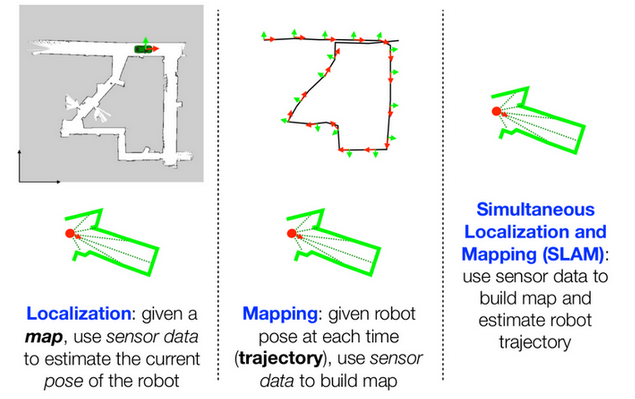
\includegraphics[width=\textwidth]{images/perception.png}
    \caption{Differenza tra localization, mapping e SLAM~\cite{f1tenthcoursel09}.}
    \label{fig:fig5} % etichetta utilizzata per riferisi all'immagine
\end{figure}

\begin{description}
    \item[Problema] -- Per determinare la posizione del robot è necessaria una mappa 
    dell’ambiente, ma si ha prima bisogno della posizione del robot per costruire la mappa stessa.
    \item[Soluzione] -- \textit{Simultaneous Localization and Mapping (SLAM)} è una tecnica che 
    consente ai robot di eseguire simultaneamente la \textit{localizzazione} e il 
    \textit{mapping} di un ambiente sconosciuto. Questo processo continua per diversi istanti 
    di tempo, aggiornando la mappa a ogni passo~\cite{f1tenthcoursel09}.
\end{description}


\subsection{Planning}
\label{subs:planning}
La \textit{pianificazione} consiste nel trovare un percorso ottimo grazie al quale il robot 
possa spostarsi progressivamente dal punto di partenza a quello di \textit{``goal''},
evitando eventuali ostacoli presenti nel cammino.

Generalmente, si suddivide quest'area di sviluppo in una gerarchia di tecniche di \textit{planning}~\cite{f1tenthcoursel12}:
\begin{itemize}
    \item \textit{Global Planner} -- Si tratta di una vista d’insieme del problema per determinare il percorso ottimo;
    \item \textit{Local Planner} -- È una vista che riguarda solo la porzione dell'ambiente 
    vicina al veicolo, sfruttata per individuare le traiettorie possibili per l'auto;
    \item \textit{Behavioral Planner} -- Consiste in una pianificazione delle strategie da 
    adottare in diverse situazioni, selezionando la migliore secondo una specifica funzione di costo.
\end{itemize}

Ad alto livello, le tecniche di pianificazione di un percorso si dividono in due categorie:
\begin{enumerate}
    \item \textit{basate sul campionamento}: \textit{Probabilistic Road Maps (PRM)} e \textit{Rapidly-Exploring Random Tree (RRT*})~\cite{samplingbased};
    \item \textit{basate sulla ricerca}: \textit{A*} e \textit{A* Lattice Planning}.
\end{enumerate}

\subsection{Control}
\label{subs:control}
% Considerare questa img: https://github.com/A-make/awesome-control-theory
Il modulo di \textit{controllo} si occupa dei segnali da inviare agli \textit{attuatori} delle 
ruote (es. angolo di sterzata, freni, ecc.) e del motore (velocità, accelerazione) per portare 
il veicolo al suo stato successivo.

In linea generale, le domande a cui si vuole rispondere sono~\cite{f1tenthcoursel10}:
\begin{itemize}
    \item Come seguire un percorso prestabilito?
    \item Come correggere gli errori di attuazione?
    \item Come guidare il veicolo il più velocemente possibile?
\end{itemize}

Si tratta di un campo di studi così vasto che viene racchiuso nella disciplina 
dell'\textit{ingegneria del controllo}~\cite{f1tenthcoursel04}, che comprende la modellazione 
di una vasta gamma di sistemi dinamici e la progettazione di controllori che garantiscano che 
questi sistemi rispettino il comportamento atteso. In particolare, se ne distinguono due tipologie differenti:
\begin{enumerate}
    \item \textit{Controller Open Loop}: sono adatti per sistemi senza vincoli di dinamica o 
    stabilità, poiché non catturano lo stato del sistema. Inoltre, attuano direttamente la risposta desiderata, senza la continua osservazione dello stato del sistema;
    \item \textit{Controller Closed Loop Feedback}: rispetto ai precedenti, sono indicati per 
    sistemi dinamici e calcolano continuamente un valore di errore $e(t)$, come differenza
    tra la risposta di output desiderata, detta \textit{setpoint}, e una variabile di processo 
    misurata che rappresenta l'output reale.
\end{enumerate}

\begin{figure}[H]
    \centering
    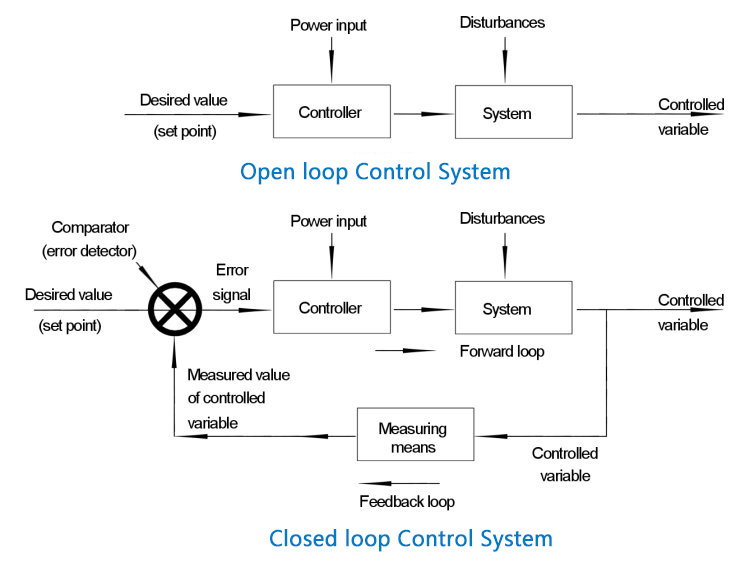
\includegraphics[width=\textwidth]{images/compare_open_closed_loop.jpg}
    \caption{Confronto tra i controller \textit{Open Loop} e \textit{Closed Loop Feedback}~\cite{diffcontrollers}.}
    \label{fig:fig6} % etichetta utilizzata per riferisi all'immagine
\end{figure}

L'obiettivo principale di un controller è quello di applicare automaticamente una 
correzione precisa e reattiva a una certa funzione di controllo, ad esempio, per mantenere
la velocità desiderata, con un ritardo e un superamento minimi, andando ad aumentare gradualmente la potenza del motore.
L’evoluzione del controllo dei veicoli autonomi può essere suddivisa in tre principali fasi di sviluppo~\cite{lect08control}:
\begin{enumerate}
    \item Ispirati dalla comunità della robotica, i primi algoritmi
    di controllo sono stati ispirati da concetti geometrici come la pianificazione di un 
    movimento circolare o l'allineamento del volante verso un percorso \textit{target}. 
    Questi approcci evidenziano buone prestazioni per velocità medio-basse.
    \item All'aumentare delle velocità e delle accelerazioni dei veicoli 
    a guida autonoma, all'interno della comunità di ricerca si sono diffusi più metodi
    di analisi approfonditi, provenienti dalla teoria del controllo e dai sistemi dinamici. 
    Permettono di progettare \textit{controllori state-feedback} e di considerarne più
    effetti dettagliati, come la dinamica dell'imbardata del veicolo e la dinamica dell'attuatore dello sterzo.
    \item Si è in seguito sviluppata una specifica branca del controllo, detta 
    \textit{controllo ottimale}, che vuole controllare un sistema in modo da minimizzare
    o massimizzare un determinato obiettivo. È particolarmente indicata per
    applicazioni complesse: infatti, fa parte di questa classe di problemi il 
    \textit{Model Predictive Control}, il tema principale studiato in questa tesi,
    che verrà discusso nel capitolo~\ref{chap:chap3}.
\end{enumerate}
Gli algoritmi di controllo trattati nel contesto di \textit{F1TENTH} comprendono 
\textit{PID Controller} e \textit{Pure Pursuit}, discussi in dettaglio nel 
Capitolo~\ref{chap:chap2}. Invece, a partire dal Capitolo~\ref{chap:chap3}, si approfondisce
\textit{Model Predictive Control (MPC)}.
\chapter{Metodi reattivi per il controllo}
\label{chap:chap2}

Questo capitolo si occupa di descrivere la navigazione con 
\textit{metodi reattivi}, in quanto rappresenta una strategia largamente 
utilizzata per il controllo di un agente autonomo. 
Essa suggerisce di prendere tutte le decisioni di controllo attraverso
un'elaborazione dei dati recenti dei sensori. 
Infatti, sono algoritmi senza un vero e proprio piano che cercano di guidare il veicolo 
evitando gli ostacoli o seguendo un percorso prestabilito -- spesso generato 
dal modulo di \textit{planning}, come spiegato nella sottosezione~\ref{subs:planning} --
fornendo input di sterzata e velocità all’auto per effettuare manovre fluide.

\section{PID Controller}
% Reactive di tipo longitudinale: determina la velocità
Una strategia semplice per far navigare l'auto consiste nel seguire una linea 
(\textit{line follow}), un muro di un corridoio o il cordolo di un circuito (\textit{wall follow}), 
attraverso un \textit{controllore} che fornisce input di \textit{sterzata} e 
\textit{accelerazione} all'auto autonoma. 

L'algoritmo più diffuso che fornisce questi input è il controllore \textit{PID},
acronimo di \textit{Proportional, Integral e Derivative}.
Si tratta di un controller molto popolare e versatile, il cui punto di forza risiede nella
sua semplicità e nei risultati che ottiene. Questo tipo di controller viene usato
nelle applicazioni che richiedono un controllo di tipo \textit{closed-loop feedback}.
Di seguito si descrive come il controllore calcola l'angolo di sterzata e la velocità
a cui guidare per poter eseguire una manovra \textit{fluida}.
\subsection{Struttura}
Il controllore acquisisce in ingresso un valore e lo confronta con un valore di 
riferimento, detto \textit{setpoint}. La differenza tra questi due valori corrisponde 
al segnale di \textit{errore}, che viene usato per determinare il valore di uscita del controllore.

Il controller \textit{PID} regola l’uscita in base ai seguenti parametri:
\begin{enumerate}
    \item il valore del segnale di errore (azione proporzionale);
    \item la somma degli errori accumulati nel tempo fino all'istante corrente (azione integrale);
    \item la velocità di variazione del segnale di errore (azione derivata).
\end{enumerate}

\begin{figure}[H]
    \centering
    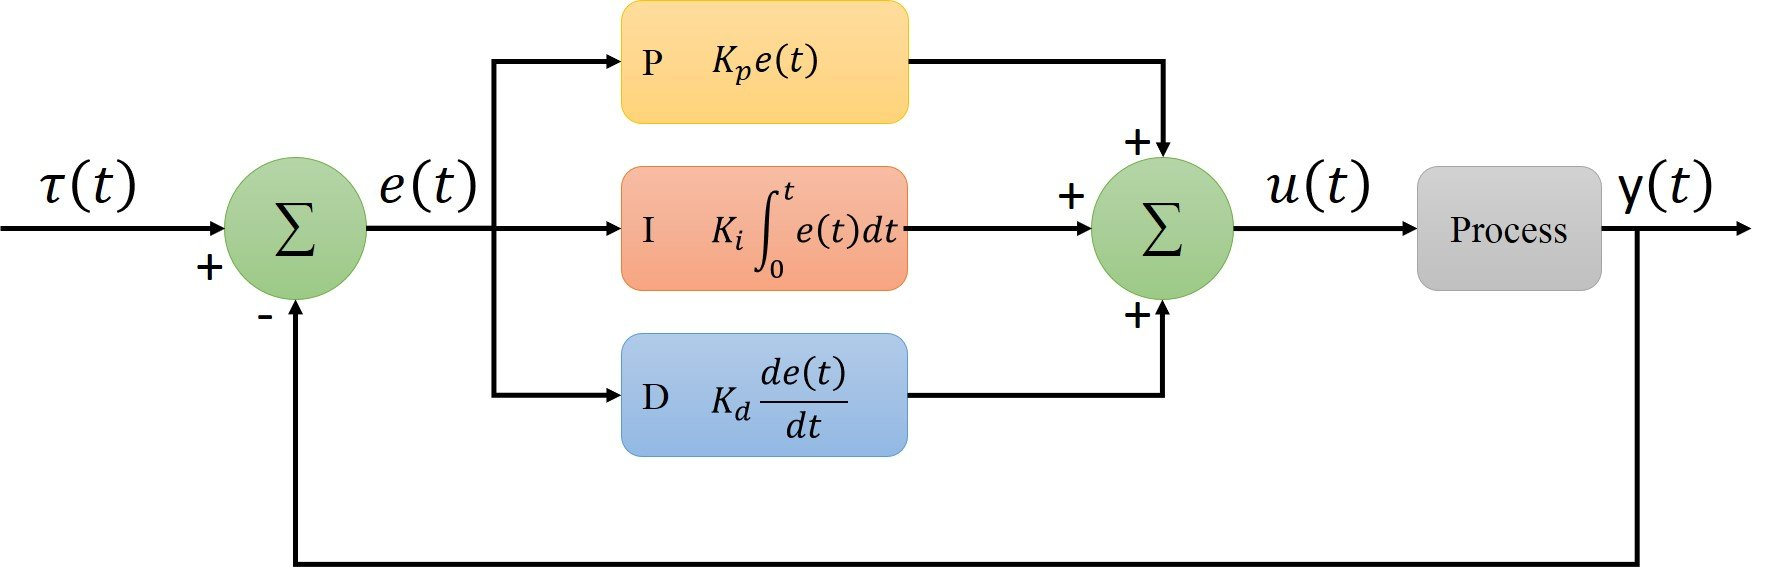
\includegraphics[width=\textwidth]{images/PID_controller.jpg}
    \caption{Schema a blocchi del PID controller. Qui $\tau(t)$ è il setpoint, $u(t)$ è l'output di controllo, mentre $y(t)$ è il valore della variabile di processo~\cite{pidimg}.}
    \label{fig:fig7} % etichetta utilizzata per riferisi all'immagine
\end{figure}
Nello specifico, le componenti di controllo del \textit{PID} sono:
\begin{itemize}
    \item \verb|Proportional Controller| -- l'angolo di sterzata dell'auto deve essere proporzionale 
    alla distanza della stessa dal percorso stabilito, detta \textit{crosstrack error}. 
    Maggiore è l’errore, maggiore deve essere la correzione per correggerlo.
    \item \verb|Derivative Controller| -- lo svantaggio principale del \verb|Proportional|
    è che provoca continue oscillazioni attorno alla linea centrale e aumenta 
    l'\textit{overshoot}, cioè il superamento del \textit{setpoint}. 
    Quello che si desidera, invece, è che l'errore diminuisca nel tempo, riducendo di 
    conseguenza anche l'azione correttiva.
    Prevenendo quest'effetto, si applica una correzione anticipata, che deve essere
    proporzionale alla velocità con cui l’errore si sta riducendo.
    Una previsione triviale è data dall’attuazione di un \verb|gain| basato sull’errore, che
    porterà il robot a controsterzare e ad avvicinarsi progressivamente alla linea centrale. 
    Dunque, l'azione derivata prevede il comportamento del sistema e ne migliora la stabilità.
    \item \verb|Integral Controller| -- è possibile includere anche un termine di 
    \verb|gain| integrale, che è proporzionale all’errore accumulato a partire da un tempo
    di riferimento $t$. L'azione integrale, dunque, tiene conto del \textit{crosstrack error} 
    accumulato nel tempo, correggendo gli errori che non sono stati risolti nei passi temporali precedenti.
\end{itemize}
L'output di controllo $u(t)$ di quest'algoritmo, vale a dire ciò che viene controllato, è 
l'angolo di sterzata $\delta$ a cui si vuole che l'auto guidi. 
Si può così indicare di seguito l'equazione standard di \textit{PID}, dove $e(t)$ è 
l'errore dalla traiettoria desiderata:
\[
u(t) = K_p e(t) + K_d \frac{de(t)}{dt} + K_i \int_{0}^{t} e(t) \,dt
\]
Le \textit{costanti} $K_p$, $K_i$ e $K_d$ determinano con quale peso contribuisce ciascuna delle tre componenti.
Nell'implementazione di PID, l'azione \textit{integrale} non è sempre necessaria.
Infatti, a seguito di una grande variazione del \textit{setpoint}, il termine integrale
può accumulare un errore superiore al valore massimo della variabile di controllo,
portando il sistema in \textit{overshooting}, con conseguente aumento dell'errore.
La soluzione a questo problema consiste nel disabilitare l'azione integrale~\cite{f1tenthcoursel04}.

Ricapitolando, il \verb|Proportional| svolge la maggior parte del lavoro, 
il \verb|Derivative| agisce sul primo per ridurne l'\textit{overshoot} e 
l'\verb|Integral|, se presente, riduce l'errore che resta dopo che il primo ha svolto il suo lavoro.

\subsection{Tuning}
Il \textit{PID} è un esempio di metodo di controllo libero da qualsiasi tipo di \textit{modello}: 
non si modella il veicolo e quindi, per ottimizzare i valori dei \verb|gain| di controllo 
$K_p$, $K_i$ e $K_d$, bisogna fare affidamento sull'esperienza e sull'analisi.
Un ingegnere del controllo deve sapere cosa si può fare, cosa non è sicuro e quali bias
sono presenti nel sistema, tuttavia molto dipende anche dalle caratteristiche prestazionali desiderate. 
Esistono sia approcci manuali che euristiche, come quella di \textit{Ziegler-Nichols}. Nell'ambito di F1TENTH, il metodo più comune è quello manuale, soprattutto in ambiente 
simulativo, come in questo caso. Con un divario inferiore tra la simulazione e la realtà 
(\textit{Sim2Real}), il codice sviluppato nel simulatore potrebbe essere utilizzato direttamente sull'auto reale.

\section{Pure Pursuit}
Il metodo del \textit{Pure Pursuit} è uno degli approcci più diffusi nella guida
autonoma per il problema affrontato in questa tesi: il \textit{path tracking} per
auto autonome da corsa.
Al veicolo viene assegnata una sequenza di posizioni da seguire, dette \textit{waypoint},
indicate nel frame di riferimento del veicolo e l'obiettivo dell'algoritmo consiste nel seguirli.

Il controllo del movimento di un veicolo \textit{olonomico} è più semplice: essi possono muoversi in 
qualsiasi direzione, a prescindere dall'orientamento del veicolo. Tuttavia, in questo contesto si ha un
veicolo non olonomico, cioè l'automobile di \textit{F1TENTH}, che deve riposizionarsi e cambiare direzione per spostarsi in un 
certo punto. Ciò, infatti, complica il problema del \textit{path tracking}.

Per affrontare questa sfida, \textit{Pure Pursuit} calcola geometricamente 
la curvatura di un arco che collega la posizione dell'asse posteriore dell'auto a un punto di 
\textit{goal} sul percorso da seguire. Quest'ultimo è sempre il \textit{waypoint} più vicino
al veicolo e ad almeno una data distanza di \textit{lookahead}, che va dalla posizione corrente
dell'auto al percorso desiderato.
In questo contesto, \textit{Pure Pursuit} rappresenta un controller laterale che ignora le 
forze dinamiche che agiscono sui veicoli e presuppone che le ruote mantengano la condizione 
antiscivolo (\textit{no-slip}).

L'algoritmo è un \verb|P Controller| dell'angolo di sterzata $\delta$ che agisce sull'errore
di tracking, secondo un certo \verb|gain| e \textit{lookahead}. 
%In breve, il puro controllo dell'inseguimento funziona come un controllore proporzionale dell'angolo di sterzata agendo sull'errore di traslazione
Per determinare l'angolo, si calcola come segue la curvatura dell'arco $\gamma$:
\begin{equation}
    r = \frac{L^2}{2|y|} \rightarrow \gamma = \frac{1}{r} = \frac{2|y|}{L^2}
\end{equation}
Il \textit{lookahead} è sempre soggetto a operazioni di \textit{tuning}: 
con un valore basso si ha un tracciamento più accurato, ma più oscillazioni;
invece se più alto, si osservano meno oscillazioni, ottenendo però un peggioramento del 
tracciamento. Infine, viene attuata la velocità che è indicata per ogni waypoint del percorso.
%\textit{Pure Pursuit} è un controller per il path tracking geometrico che si basa sul nostro modello di veicolo per selezionare i comandi di sterzata.
%Quest'algoritmo è stato originariamente concepito come metodo di controllo per calcolare l'arco necessario per riportare un robot su un percorso.
\section{Vantaggi e svantaggi}
I \textit{vantaggi} dei \textit{metodi reattivi per il controllo} comprendono: 
\begin{enumerate}
    \item la possibilità di applicarlo a robot con risorse hardware limitate e a basso prezzo;
    \item il fatto di poter far navigare un robot in sicurezza in ambienti completamente 
    sconosciuti e contenenti ostacoli non prevedibili.
\end{enumerate}
Invece, tra gli \textit{svantaggi} di questi metodi si ha che:
\begin{enumerate}
    \item possono occasionalmente far seguire traiettorie \textit{impraticabili} per i robot, 
    dunque non è facile adattarli a sistemi più complessi;
    \item i \verb|gain| di controllo devono essere regolati manualmente e per diverso tempo, 
    comportando un'intensa attività di \verb|tuning|;
    \item un'eventuale suddivisione del problema in due diversi controllori 
    (\textit{longitudinale} e \textit{laterale}) ignorerebbe l'accoppiamento tra le due 
    dimensioni. Ciò comporterebbe che, per esempio, il controllore \textit{PID}, usato solo 
    come controllore longitudinale, non sappia nulla del controllore laterale 
    (\textit{Pure Pursuit}). In certe situazioni, come in una curva, ciò può generare problemi nella sterzata;
    \item non offrono alcuna possibilità di gestione dei vincoli;
    \item considerano solo lo stato attuale e, dunque, ignorano le decisioni future. In questo modo, non considerano le conseguenze che possono avere le decisioni attuali sulle successive.
\end{enumerate}
Come anticipato nella sottosezione~\ref{subs:control}, \textit{Model Predictive Control} 
costituisce una soluzione più avanzata che permette di superare i limiti dei metodi reattivi, 
poiché ha alla base il \textit{controllo ottimale}.
\chapter{Model Predictive Control}
\label{chap:chap3}

In questo capitolo si approfondisce il lavoro principale di questa tesi che,
come anticipato in precedenza, è stato lo studio e l'implementazione di un sistema
di \textit{path tracking} che permettesse al veicolo di seguire
un percorso -- composto da una serie di \textit{waypoint} equidistanti -- mediante 
un tracking preciso della traiettoria di riferimento, eventualmente tentando anche di 
ridurre i tempi di completamento di un giro su specifici circuiti da corsa.

Per raggiungere questo scopo, si è scelto di realizzare 
\textit{Model Predictive Control} (\textit{MPC}), 
un controller all’avanguardia che, generalmente, viene progettato per 
automatizzare un sistema di \textit{sensori} e \textit{attuatori},
come sistemi energetici industriali o robotici.
Tra l'altro, anche Ayrton Senna, uno dei più grandi piloti di Formula 1 
di tutti i tempi, andava ad applicare una strategia simile a \textit{MPC}, attraverso la 
\textit{tecnica dell’acceleratore}. In pratica, Senna aveva un modello mentale del 
comportamento del turbocompressore e, in modo predittivo, cercava di massimizzare 
l’accelerazione in uscita da una curva~\cite{f1tenthcoursel13}.

Le metodologie basate su \textit{MPC} rappresentano la soluzione principale alla base di 
diversi controller per veicoli da corsa autonomi che sono stati implementati su veicoli reali~\cite{Betz2022}.
Più precisamente, si tratta di una strategia di controllo che sfrutta un 
determinato \textit{modello della dinamica dell’ambiente} e, rispettando una serie di 
\textit{vincoli}, è in grado di controllare un dato processo. 
Il modello deve essere adeguato al sistema o processo da controllare poiché uno
dei vincoli da soddisfare è proprio il modello. Pertanto, esso viene utilizzato per 
prevedere il comportamento futuro con l'\textit{obiettivo} di trovare l'input di controllo 
\textit{ottimale}, che deve essere applicato per un certo \textit{orizzonte temporale} scelto.

Nel contesto di questa tesi e di \textit{F1TENTH}, lo scopo di \textit{MPC} è generare,
per $N$ passi futuri, controlli di input validi che guidino il veicolo il più vicino 
possibile alla traiettoria di riferimento, garantendo al contempo prestazioni stabili anche a 
velocità sostenute.
Come accennato, \textit{MPC} è in grado di gestire i vincoli del sistema, cosa che non è 
possibile con un metodo reattivo come il \textit{PID}. Quest'ultimo, infatti, è un sistema
di tipo \textit{SISO} (\textit{Single Input, Single Output}), in grado di gestire
solo un singolo input $e(t)$ e generare un singolo output $u(t)$. Un esempio può essere 
l'avere come input l'errore dell'angolo di sterzata e come output il calcolo del nuovo angolo di sterzata.

Quindi, tra i due, conviene adottare \textit{MPC}, anche perché le dinamiche dell’ambiente
possono cambiare nel tempo e \textit{MPC} offre un modo semplice per stimare tali dinamiche e 
adeguarsi correttamente. Al contrario, \textit{PID} non è adatto per i sistemi la cui
dinamica cambia frequentemente, perché potrebbe essere necessario modificare 
continuamente i valori dei \verb|gain| di controllo per ottenere il comportamento
desiderato, rischiando comunque di imbattersi in un \textit{overshoot}.
Inoltre, a differenza di \textit{PID}, \textit{MPC} è dotato di un vettore di 
\textit{input di controllo} e di un vettore di \textit{stato}, dunque è un sistema di tipo 
\textit{MIMO} (\textit{Multi-Input, Multi-Output}), che consente cioè a più input di variare l’output del sistema.

Un'alternativa di tipo \textit{MIMO} a \textit{MPC} è \textit{LQR} 
(\textit{Linear Quadratic Regulator}), una versione senza vincoli 
e più semplice di MPC~\cite{f1tenthcoursel13}, che però ha i seguenti limiti:
\begin{enumerate}
    \item non è in grado di gestire dei vincoli;
    \item può generare input di controllo impraticabili per il robot, come un angolo di sterzata di $\frac{\pi}{2}$.
\end{enumerate}
\textit{MPC} risulta quindi essere un controllore che permette di soddisfare:
 \begin{enumerate}
     \item vincoli di \textit{sicurezza}, come velocità, accelerazione e limiti del percorso;
     \item vincoli \textit{fisici}, come mantenere una traiettoria possibile per la dinamica dell'auto.
 \end{enumerate}

 % Valutare se inserire questa img:
%https://docs.google.com/presentation/d/1QBXVAaRjFa0_fBHOmTFo2AHS1nvde_nONzNAGvCgCxM/edit#slide=id.g21997f8dc71_0_142

\section{Struttura}
Dopo aver analizzato le problematiche di altri metodi e aver introdotto \textit{MPC}, si vuole 
comprendere come controllare all'ottimo un sistema.
Infatti, il primo passo per impostare \textit{MPC} è definire il problema di controllo ottimale
da risolvere, che è caratterizzato dalle seguenti componenti:
\begin{enumerate}
    \item il \textit{modello} della dinamica del sistema, per prevedere il comportamento futuro.
    \textit{Esempio}: dinamica del veicolo;
    \item la \textit{funzione obiettivo} da minimizzare. \textit{Esempio}: \textit{cross-track error} e/o tempo di un giro;
    \item i \textit{vincoli} da rispettare all'interno del sistema. \textit{Esempio}: limiti della velocità, della sterzata, ecc.
\end{enumerate}
Pertanto, si tratta di un problema di \textit{ottimizzazione convessa} con vincoli e ciò 
che si vuole risolvere è la sequenza $[x_0 \ ... \ x_N \ \ \ \ u_0 \ ... \ u_N]^T$, composta da:
\begin{enumerate}
    \item azioni di controllo, indicate come $u$;
    \item stati previsti, indicati come $x$.
\end{enumerate}
Come anticipato, \textit{MPC} si prefigge di controllare un sistema risolvendo iterativamente un 
problema di ottimizzazione che sia in grado di prendere in considerazione un modello e dei vincoli fisici. 
Il controllore ha il compito di minimizzare una certa funzione obiettivo, detta anche di costo, 
attraverso la simulazione degli stati futuri, a partire da quello attuale e dalle variabili di 
controllo, secondo uno specifico modello del sistema.
Questi stati sono delimitati dai vincoli dati a \textit{MPC} in modo che non vengano raggiunti stati indesiderati e/o non praticabili. 
Le variabili di controllo possono quindi essere scelte in 
modo che gli stati generati soddisfino la funzione di costo. 

Il punto nel futuro fino al quale simula viene determinato da un \textit{orizzonte} di previsione 
finito: per un orizzonte più ampio il tracciamento risultante sarebbe certamente più fluido, 
ma anche più pesante a livello computazionale.
Le variabili di controllo calcolate possono quindi essere utilizzate come attuazione per il 
sistema controllato in quell'istante di tempo~\cite{racelinecontrol}.

\begin{figure}[H]
    \centering
    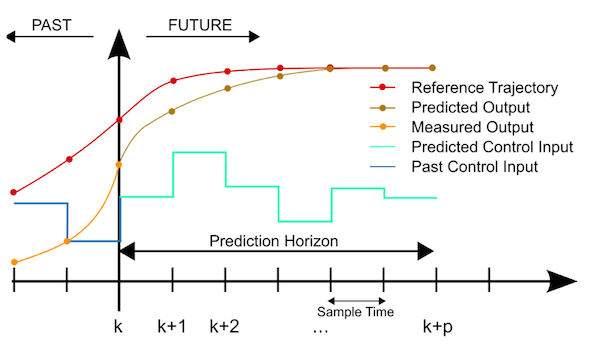
\includegraphics[scale=0.7]{images/mpc_prediction.png}
    \caption{Diagramma che mostra il lavoro 
    svolto da \textit{MPC}, differenziando tra 
    \textit{passato} e \textit{futuro} (con un certo orizzonte)~\cite{mpschema}.}
    \label{fig:fig8} % etichetta utilizzata per riferisi all'immagine
\end{figure}

Nella Fig.~\ref{fig:fig8} si può osservare
che la linea azzurra in basso è l'attuazione, 
un input di controllo discreto, mentre in alto 
si trovano sia la traiettoria di riferimento 
che quella futura prevista.
Il controllore prenderà in considerazione lo stato rilevato del sistema e 
ottimizzerà una sequenza di controllo ideale, 
in base alla funzione obiettivo definita.

Dunque, il problema di ottimizzazione con vincoli alla base di \textit{MPC} si può 
definire come la minimizzazione del costo di una traiettoria che sia praticabile per la
dinamica del sistema e che non violi i vincoli imposti. Si riporta di seguito un \textit{setup} 
generale di questo problema:
\[
\begin{aligned}
U_t^*(x(t)) := \min_{U_t} &\sum_{k=0}^{N-1} q(x_{t+k}, u_{t+k}) \\
\text{subject to } & x_t = x(t) & \quad & \text{misure} \\
& x_{t+k+1} = Ax_{t+k} + Bu_{t+k} & \quad & \text{modello del sistema} \\
& x_{t+k} \in \mathcal{X} & \quad & \text{vincoli dello stato} \\
& u_{t+k} \in \mathcal{U} & \quad & \text{vincoli degli input} \\
& U_t = \{u_t, u_{t+1}, \ldots, u_{t+N-1}\} & \quad & \text{variabili di ottimizzazione}
\end{aligned}
\]
Si specifica che con $k = 0$ si intende il time-step corrente, mentre con $k = N-1$ si fa 
riferimento al time-step antecedente alla fine della finestra dell'orizzonte temporale. 
Si discuterà maggiormente del tema nelle sezioni successive, entrando nello specifico di ciascuna 
componente del problema di ottimizzazione.

\subsection{Receding Horizon Control}
Alla base del funzionamento di \textit{Model Predictive Control} c'è il concetto di orizzonte finito, definito in letteratura come \textit{Receding Horizon Control}. 
Questo indica che, dopo che è stata applicata l'attuazione, viene calcolata una nuova serie di 
variabili di controllo per il nuovo stato del veicolo. 
\begin{figure}[H]
    \centering
    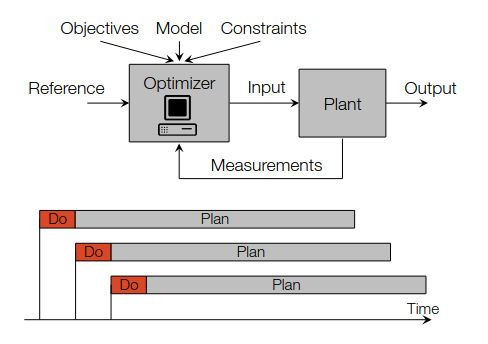
\includegraphics[scale=0.6]{images/mpc_horizon.png}
    \caption{Struttura di \textit{MPC con Receding Horizon Control}, in cui si pianifica per una 
    certa finestra di tempo~\cite{f1tenthcoursel13}.}
    \label{fig:fig9} % etichetta utilizzata per riferisi all'immagine
\end{figure}
Come si può osservare dalla Fig.~\ref{fig:fig9}, ciò viene reiterato in modo da aiutare il 
controllore nella gestione di comportamenti inaspettati.
Il vantaggio principale è rappresentato dal fatto che, 
applicando continuamente gli input di controllo ottimali, 
il sistema può essere portato verso un riferimento 
desiderato -- come una traiettoria ottima da seguire -- 
che viene raggiunto quando la funzione obiettivo risulta minimizzata.

Per progettare un controllore con queste caratteristiche, il sistema deve essere di tipo 
\textit{closed loop}, cioè deve includere un meccanismo di feedback in cui le variabili di 
controllo $u$ vengono calcolate in base all'errore tra gli stati di riferimento $x_{r e f}$ e gli stati simulati $x$.
Inoltre, l’orizzonte finito consente di avere un problema di ottimizzazione trattabile 
computazionalmente, in contrapposizione al controllo dell’orizzonte infinito 
(con un sistema \textit{``open loop''}), che risulterebbe impraticabile poiché 
considererebbe tutto l'ambiente -- il circuito in questo contesto -- e non più solo una parte di esso.

Più precisamente, i passi dell’\textit{MPC} con orizzonte finito sono i seguenti~\cite{mpcpeters}:
\begin{enumerate}
    \item Ottenere lo stato corrente $x(t)$;
    \item Calcolare, per una determinata finestra di pianificazione 
    temporale $N$, la sequenza di input di controllo ottimale: 
    $U^*_{t} = \{u^*_{t},\dots, u^*_{t+N-1}\}$;
    \item Applicare solo il primo input di controllo $u^*_{t}$;
    \item Ripetere per ripianificare.
\end{enumerate}
L'intuizione fondamentale è che, invece di applicare l'intera sequenza di input calcolata, si 
applichi solo il primo input ottimale per poter istantaneamente misurare lo stato risultante del veicolo. 
In questo modo si riescono a considerare preventivamente gli errori poiché viene introdotto un
feedback grazie alla successiva ripianificazione.

È presente un trade-off nella scelta dell'orizzonte di pianificazione $N$: idealmente, se ne 
vorrebbe avere uno breve che consideri pochi istanti temporali, risultando anche più leggero; 
tuttavia, con un orizzonte troppo ridotto la traiettoria pianificata potrebbe non tenere conto del 
comportamento futuro del sistema, portando il controllore a intraprendere azioni di controllo 
miopi -- ad esempio, mantenere un'accelerazione elevata in prossimità di una curva che non è stata rilevata.
D'altro canto, un orizzonte che guarda troppo in avanti renderebbe impegnativo il raggiungimento
di soluzioni precise, sia per ciò che riguarda la funzione di costo che per il rispetto dei vincoli.

\section{Modello}
Per poter formulare un problema di controllo ottimale, è necessario disporre di un 
\textit{modello della dinamica del sistema}, poiché esso è in grado di prevedere l'evoluzione 
dello stato del veicolo per una sequenza di input data in ingresso.
Questo modello può essere rappresentato dalla seguente equazione:
\[ \dot{x}(t) = f(x(t), u(t)) \]
dove $x(t) \in \mathbb{R}^n$ è lo stato del sistema, 
$u(t) \in \mathbb{R}^m$ rappresenta gli input di controllo e 
$f : \mathbb{R}^n \times \mathbb{R}^m \rightarrow \mathbb{R}^n$ è 
la funzione di sistema, cioè il modello della dinamica~\cite{f1tenthcoursel13}. 
Non è possibile risolvere l'equazione analiticamente in forma chiusa, 
pertanto deve essere risolta numericamente. Passando dal continuo al
discreto, dunque si ottiene:
\[ x_{t+1} = f(x_t, u_t) \]
con $t \in \mathbb{N} $. Si approfondirà il processo di discretizzazione nella sezione~\ref{sect:disc}.

Nello specifico, il modello della dinamica $f$ prende lo stato
$x_t$ -- ad esempio, corrispondente alla posizione e alla velocità dell'auto -- e gli input di controllo -- ad esempio, corrispondenti all'angolo di sterzata e all'accelerazione -- e li mappa 
allo stato dell'istante di tempo successivo. 
In altre parole, data una sequenza di input e, soprattutto, un modello
si può prevedere l'evoluzione dello stato nel futuro.

Il modello della dinamica del sistema appena descritto è necessario affinché il controllore 
sia in grado di simulare correttamente il cambiamento nello stato del veicolo.
Più precisamente, questo modello è caratterizzato da una serie di equazioni differenziali che descrivono 
questo cambiamento in ciascuna variabile di stato. Esistono diverse semplificazioni del modello, 
alcune più dettagliate e altre meno, ma tutte comprendono sempre il comportamento generale del veicolo.
Questi ``rilassamenti'' del modello sono utili perché è difficile modellare precisamente un veicolo
reale. Oltre a ciò, al crescere della complessità del modello cresce rapidamente anche quella del controllore.

\subsection{Kinematic Bicycle Model}
\label{subs:kinmodel}
La modellazione del comportamento dinamico del veicolo è una parte cruciale nel campo delle auto da corsa a guida autonoma.
Questi modelli vengono utilizzati sia negli ambienti di simulazione che in lavori riguardanti la
progettazione del controllo della traiettoria, proprio come fatto in questo lavoro di tesi.

Lo stato dell'arte al momento offre molti modelli diversi tra loro, 
come il \textit{Kinematic Bicycle Model}, \textit{Dynamic Bicycle 
Model}, il \textit{Double Track Model} o il \textit{Full Vehicle 
Model}. Più il modello della dinamica del veicolo è complesso, più aumentano i parametri necessari per la sua realizzazione~\cite{Betz2022}.

Il modello scelto per questa tesi è il primo, anche detto \textit{Kinematic Single-Track Model} e \textit{Front Wheel Steering Model} in letteratura. 
Esso può essere definito come un modello semplificato che cattura molto bene il movimento del veicolo.
Nel concreto, il modello ``rilassa'' il concetto di veicolo attraverso l'unione delle due ruote 
anteriori in un'unica ruota; stesso discorso per quelle posteriori. 
\begin{figure}[H]
    \centering
    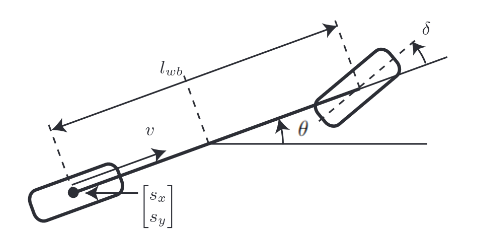
\includegraphics[scale=0.8]{images/kin_model.png}
    \caption{\textit{Kinematic Bicycle Model} con punto di riferimento al centro dell'asse posteriore~\cite{Althoff2017a}.}
    \label{fig:fig10} % etichetta utilizzata per riferisi all'immagine
\end{figure}
Come visibile in Fig.~\ref{fig:fig10}, questa configurazione a due ruote permette di paragonarlo proprio a una \textit{bicicletta}; il modello infatti copre solo il movimento su un piano, 
ignorando di conseguenza i movimenti di rollio e beccheggio. Inoltre, può differire leggermente
a seconda che le variabili di input siano la velocità e la sterzata, o l'accelerazione e la sterzata (come in questo caso).
L'orientamento della ruota anteriore può essere controllato rispetto alla 
direzione del veicolo, mentre non è possibile lo stesso ragionamento
per la ruota posteriore; dunque, di fatto, si considera e si segue solo la ruota anteriore~\cite{Althoff2017a}.

Per formalizzare il \textit{``Kinematic Bicycle Model''}, bisogna 
innanzitutto definire lo spazio degli stati come 
$x=[s_x, s_y, \theta, v]$, dove $s_x$ e $s_y$ sono
le coordinate del veicolo poste al centro dell'asse posteriore, 
$\theta$ è l'orientamento del veicolo e $v$ la velocità; dopodiché, si
definisce il vettore degli input come $u=[a, \delta]$, dove $a$ 
rappresenta l'accelerazione e $\delta$ l'angolo di sterzata delle 
ruote anteriori.
Le equazioni differenziali che descrivono il cambiamento di stato per il modello sono:
\[
\dot{s}_x=v\cos(\theta), \quad
\dot{s}_y=v\sin(\theta), \quad
\dot{v}=a, \quad
\dot{\theta}=\frac{v\tan(\delta)}{l_{wb}}
\]
Dove $l_{wb}$ indica la lunghezza del passo (\textit{wheelbase}) del 
veicolo da una ruota all'altra e corrisponde a 
$l_\text{front} + l_\text{rear}$. 
Le equazioni differenziali indicate sopra si possono esprimere in 
forma sintetica come:
\[ \dot{x} = f(x, u) = A'x + B'u \]
Dove $A'$ e $B'$ sono matrici di sistema continue e, come anticipato, il sistema verrà poi discretizzato (sezione \ref{sect:disc}) e linearizzato (sezione \ref{sect:lin}).

Il modello cinematico ignora l'effetto dello slittamento degli pneumatici e quindi non riflette in 
certi casi la dinamica effettiva~\cite{jain2020bayesrace}. 
In genere, è particolarmente indicato in condizioni di guida normali, tuttavia un modello più 
complesso, come quello dinamico, non necessariamente migliorerebbe le prestazioni poiché potrebbe 
richiedere maggior tempo per la risoluzione. 
Tuttavia, in alcuni casi il modello cinematico può risultare adeguato anche in condizioni di guida 
più estreme; in caso contrario, il modello necessita di una buona rapidità per riuscire a compensare i segnali di controllo non ottimali.

\section{Funzione Obiettivo}
\label{subs:obj}
Il compito della \textit{funzione obiettivo} è quello di assegnare un \textit{costo} $J$
a una traiettoria data, in modo da valutare la bontà di quest'ultima per lo scopo prefissato. 
Considerando $T$ come il numero di passi dell'orizzonte temporale, tale costo può essere espresso come:
\[
\begin{aligned}
J = & \sum_{t=0}^{T}c_t(x_t, u_t) = \\ &
\ Q_{f}\left(x_{T}-x_{T, r e f}\right)^{2}+ \\ & Q \sum_{t=0}^{T-1}\left(x_{t}-x_{t, r e f}\right)^{2}+ \\ & R \sum_{t=0}^{T} u_{t}^{2}+R_{d} \sum_{t=0}^{T-1}\left(u_{t+1}-u_{t}\right)^{2}
\end{aligned}
\]
L'obiettivo consiste nel minimizzare il costo $J$. Si noti che $J$ è quadratica ed è divisa in due parti~\cite{f1tenthcoursel13}:
\begin{enumerate}
    \item \textit{Costo dell'errore di stato}, pesato dalla matrice di peso $Q$ e $Q_f$;
    \item \textit{Costo dell'attuazione}, pesato dalle matrici di peso $R$ e $R_d$. 
\end{enumerate}
Nello specifico, la funzione di costo penalizza sia la differenza tra gli stati calcolati e gli 
stati di riferimento, sia i grandi input di controllo, affinché lo stato desiderato venga 
raggiunto con un input di controllo minimo. Si vogliono infatti minimizzare tre sotto-obiettivi:
\begin{enumerate}
    \item La deviazione del veicolo dalla traiettoria di riferimento: $\forall t \in T, \ x_t-x_{t, r e f}$. 
    La deviazione dello stato finale è pesata da $Q_f$, mentre le altre da $Q$.
    \item Il fattore di influenza degli input di controllo,
    pesato da $R$.
    \item La differenza tra un input di controllo e il successivo, pesata da $R_d$.
\end{enumerate}
Le matrici di pesi $R$, $R_d$ e $Q$ giocano un ruolo fondamentale nel determinare il comportamento
di \textit{MPC}. Esse infatti influenzano il modo in cui l'algoritmo penalizza, rispettivamente, l'attuazione 
degli input di controllo, i cambiamenti negli input di controllo e la deviazione dalla traiettoria di riferimento.
In \textit{MPC}, la matrice $Q$ è sempre semi-definita positiva; ciò garantisce che il costo 
associato agli errori di stato non sia mai negativo, il che è importante per mantenere la 
convessità del problema di ottimizzazione e per garantire che il costo totale non sia appunto negativo.
Invece, la matrice $R$ è sempre definita positiva, garantendo quindi che ci sia sempre un costo associato 
all'applicazione degli input di controllo, evitando così soluzioni banali senza penalità in cui gli input
di controllo potrebbero essere troppo grandi o piccoli. 

Più precisamente, valori più alti per $R$ indicano che l'algoritmo sarà più riluttante a 
utilizzare input di controllo elevati; la matrice $R_d$ può aiutare a ottenere un controllo più 
fluido; infine, le matrici $Q$ e $Q_f$ riducono la deviazione dalla traiettoria di riferimento da seguire.
\section{Vincoli}
Come già anticipato a inizio capitolo, uno dei vantaggi più significativi di \textit{MPC} è 
proprio la possibilità di gestire i \textit{vincoli} del sistema trattato. 
Ciò permette di riflettere in modo più preciso la realtà rispetto a un metodo reattivo come
il \textit{PID Controller}, trattato nel Capitolo~\ref{chap:chap2}.
I vincoli del problema di ottimizzazione sono i seguenti:
\begin{itemize}
    \item lo \textit{stato iniziale} in programma per l'orizzonte corrente deve corrispondere allo 
    stato corrente del veicolo, cioè $x_0 = x(0)$. Quindi, lo stato iniziale $x_0$ è 
    impostato come lo stato corrente del veicolo, mentre il tempo iniziale corrisponde al tempo 
    nello stato di riferimento più vicino allo stato corrente del veicolo.
    \item gli \textit{stati futuri} del veicolo devono seguire il modello della dinamica del veicolo \textit{linearizzato}.
    \item gli \textit{input generati} non devono superare i limiti fisici del veicolo.
\end{itemize}

\subsection{Stati futuri e dinamica}
Un modello che prevede stati $x$ futuri può mutare nel tempo. Alcuni risolutori moderni
possono gestire dinamiche non lineari -- ad esempio \textit{Casadi}, che non è stato però oggetto 
di questo lavoro -- tuttavia spesso si cerca di linearizzare la dinamica del sistema per 
effettuare il calcolo di \textit{MPC} in modo più veloce. La dinamica linearizzata è solitamente nella seguente forma:
\[
x_{t+1} = Ax_t+Bu_t \quad \forall x,u \in [x_0 \ ... \ x_N \ \ \ \ u_0 \ ... \ u_N]^T
\]
% Valutare se usare $k$ o $t$
Questo vincolo su due stati consecutivi, vale a dire $x_t$ e $x_{t+1}$, garantisce che la sequenza 
degli stati possa essere esclusivamente una \textit{traiettoria realistica} che rispetta la 
dinamica del sistema.

\subsection{Stato e input}
I vincoli per stato e input possono essere formulati semplicemente come un limite inferiore e 
superiore su una delle variabili di stato o di controllo.
Alcuni esempi di vincoli di disuguaglianza sono dati da:
\begin{itemize}
    \item \textit{Limiti dell'attuatore} -- in riferimento all'angolo di sterzata, alla velocità, ecc.
    \item \textit{Confini del tracciato} -- può essere interpretato come una regione delimitata da un insieme di linee.
\end{itemize}
Dunque, i vincoli del sistema codificano i domini degli stati
$x_t \in \mathcal{X}$ e degli input $u_t \in \mathcal{U}$ 
consentiti.
Ciascun vincolo di disuguaglianza può essere scritto come $Ax \le b$, dove per ogni riga di $A$, b corrisponde a un vincolo applicato.

\section{Algoritmo}
Si mostra di seguito lo pseudocodice del funzionamento generale dell'algoritmo del 
\textit{Model Predictive Control} che, ricevendo in ingresso la funzione di costo $J$, il modello 
della dinamica del sistema $f$, l'orizzonte degli eventi $T$ e l'input di controllo iniziale
$\hat{u}_0$, risolve all'ottimo il problema.
%\algrenewcommand{\algorithmiccomment}[1]{\hfill// #1}
\begin{algorithm}[H]
\caption{MPC: Model Predictive Control}\label{alg:mpc}
\begin{algorithmic}[1]
\Require Obiettivo $J$, modello della dinamica $f$, orizzonte temporale $T$,
input di controllo iniziale $\hat{u}_0$.
\State $u_t \gets \hat{u}_0$

\While{True}
    \State $x_{0} \gets$ \Call{GET\_CURRENT\_STATE}{}()
    \LComment{Il risolutore viene settato in warm-start, così da sfruttare la soluzione dell'iterazione precedente.}
    \State $u_t \gets$ \Call{SOLVE\_LINEAR\_MPC}{$J, f, x_0, T, u_t$}
    \State $u \gets$ \Call{GET\_FIRST}{$u_t$}
    \State \Call{EXECUTE\_CONTROL}{u}
\EndWhile
\end{algorithmic}
\end{algorithm}
Prima di farlo però, come si può vedere nell'algoritmo~\ref{alg:mpc}, l'input di controllo viene inizializzato con quello iniziale. In 
seguito, dentro il ciclo viene rilevato lo stato corrente $x_0$, che viene poi passato in input al 
risolutore, insieme agli altri componenti principali del problema di ottimizzazione.

Una volta fatto ciò, si ottiene la sequenza di controlli ottimale. Si noti però come l'algoritmo
sfrutta e attua solo il primo di questi input, che corrisponde al primo passo temporale della 
finestra dell'orizzonte data.

Dato che i controlli tra un passo temporale e il successivo variano di poco, si sfrutta il
concetto di \textit{warm start}: si riutilizza l'input di controllo dell'iterazione precedente in 
modo da trovare la soluzione del passo successivo in modo più rapido. In questo modo l'intero 
algoritmo trarrà beneficio da questa caratteristica, richiedendo tempi di calcolo inferiori.

\section{Quadratic Programming}
Il problema di ottimizzazione che caratterizza \textit{MPC} non ha soluzioni analitiche. 
Per poterlo risolvere, infatti, bisogna formulare un problema di
\textit{Quadratic Programming (QP)}. Si tratta di un processo per risolvere problemi di 
ottimizzazione matematica che coinvolgono \textit{funzioni quadratiche}. L'obiettivo di questo 
metodo è quello di trovare un vettore $z$ che minimizzi (o massimizzi) una funzione quadratica 
soggetta a \textit{vincoli lineari} sulle variabili.
Infatti, devono essere mantenute alcune condizioni di frontiera (\textit{boundary}) durante 
l’ottimizzazione, come \textit{lower bound} e \textit{upper bound}. 
In realtà, il termine \textit{``programmazione''} in questo contesto si riferisce solo a una procedura formale usata per risolvere problemi matematici.

Avendo $c,z \in \mathbb{R}^n, A_{m \times n}, Q_{m \times n}$, una forma standard 
comune di \textit{programmazione quadratica} è la seguente:
\[
\begin{aligned}
\min \ f(z) = \frac{1}{2} z^T & Hz + c^Tz \\
\text{subject to } \ & l_b \leq A_c z \leq u_b
\end{aligned}
\]
Un'altra caratteristica di \textit{QP} è che è \textit{convessa}, cioè, esiste un \textit{unico ottimo globale}.
Si ricorda che una funzione a valori reali è detta \textit{convessa} se il segmento di linea che 
congiunge due punti qualsiasi del suo grafico giace sopra il grafico stesso (o coincide con una 
sua parte). In altri termini, se si traccia una linea tra due punti qualsiasi, la funzione sarà sotto la linea.
Inoltre, un problema di questo tipo può essere risolto efficientemente in tempo reale 
(\textit{online}). Sono disponibili molti solutori di QP, tra i quali:
\begin{itemize}
    \item \textit{OSQP}, CVXGen, QuadProg, ecc.
    \item \textit{Casadi} per l’ottimizzazione non convessa.
    \item MPT3 per la progettazione e l'analisi lineare di \textit{MPC}.
\end{itemize}
Il risolutore più consigliato da F1TENTH è \textit{OSQP (Operator Splitting Quadratic Program)}~\cite{osqp}.

Manca ancora un aspetto importante per poter formulare il problema 
come uno di \textit{QP}: bisogna prima \textit{discretizzare} il sistema dinamico 
e \textit{linearizzarlo} attorno a un certo punto.

\subsection{Discretizzazione}
\label{sect:disc}
Per effettuare quest'operazione viene utilizzata -- ma non implementato -- il metodo 
\textit{``Forward Euler''} poiché è il più semplice. Dovrebbero funzionare anche altri metodi, come \textit{RK4/6}.
Per la discretizzazione viene utilizzato il tempo di campionamento $dt$, che può essere scelto come parametro da ottimizzare. 
Si può quindi esprimere l’equazione del sistema come:
\begin{equation}
\label{eq:disc}
x_{t+1} = x_t + f(x_t, u_t) \ dt
\end{equation}

\subsection{Linearizzazione}
\label{sect:lin}
La maggior parte dei sistemi fisici sono non lineari, il che comporta che le loro equazioni sono 
più complesse da risolvere. Invece, i sistemi lineari sono più semplici, sono generalmente ben 
compresi e possono essere analizzati più agevolmente.
I sistemi non lineari possono essere ben approssimati da un sistema lineare in un piccolo intorno 
di un punto presente nello spazio degli \textit{stati}.
L'idea è quella che se il sistema viene controllato per rimanere vicino
a un punto operativo -- in una condizione di lavoro stabile -- si può poi 
sostituire il sistema non lineare con uno linearizzato attorno a quel punto.

Per la \textit{linearizzazione} si sfrutta l’espansione di Taylor del primo 
ordine della funzione a due variabili in (\ref{eq:disc}) attorno a certi $\bar{x}$ e $\bar{u}$, che
porta ad avere: 
\[
\begin{aligned}
x_{t+1}& = \ x_t + (f(\bar{x_t}, \bar{u_t}) + f'_z(\bar{x_t}, \bar{u_t})(x_t - \bar{x_t}) + f'_u(\bar{x_t}, \bar{u_t})(u_t - \bar{u_t}))dt \\
& \rightarrow \ A x_t + B u_t + C
\end{aligned}
\]
Nel contesto di \textit{MPC}, i sistemi lineari consentono di tradurre la dinamica come vincoli 
lineari secondo la formulazione di \textit{MPC}, dunque essi permettono di riscrivere \textit{MPC} come un \textit{QP} standard.
Il problema di ottimizzazione risultante è così di rapida risoluzione.

\subsection{Conversione}
Per passare dalla forma generale del problema di \textit{MPC} alla formulazione 
in programmazione quadratica si effettua principalmente un lavoro di gestione di
indici e di matrici. Per quanto riguarda la funzione di costo $J = \frac{1}{2} z^T H z + c^T z$, vale:
\[
H = \text{diag}(Q, Q, \dots, Q_N, R, \dots, R)
\]
\[
c = \begin{bmatrix}
    -Q x_r \\
    \vdots \\
    -Q_N x_r \\
    0 \\
    \vdots \\
    0
\end{bmatrix}
\quad \quad
z = \begin{bmatrix}
    x_0 \\
    \vdots \\
    x_{N+1} \\
    u_0 \\
    \vdots \\
    u_N
\end{bmatrix}
\]
$H$ è una matrice diagonale in cui ci sono $N-1$ matrici di penalità $Q$ e $N$ matrici $R$ uguali,
dove ognuna di esse fa riferimento a un \textit{timestep} preciso dell'orizzonte di MPC. Si distingue 
solo $Q_N$ perché l'ultima potrebbe avere pesi diversi.
Invece $c$ è un vettore che considera gli stati di riferimento -- dove $-Q x_r$ è 
estratto da $(x_k - x_{ref})^T Q (x_k - x_{ref})$.

Bisogna poi trasformare i vincoli della dinamica e quelli di stato e
input nella forma compatta $l_b \le A_c z \le u_b$. Per la matrice $A_c$, diversamente, si ha:
\[
l_b = \begin{bmatrix}
    -x_0 \\
    0 \\
    \vdots \\
    0 \\
    x_{\text{min}} \\
    \vdots \\
    x_{\text{min}} \\
    u_{\text{min}} \\
    \vdots \\
    u_{\text{min}}
\end{bmatrix}
\quad
A_c = \begin{bmatrix}
    -I & 0 & 0 & \dots & 0 & 0 & 0 & 0 \\
    A & -I & 0 & \dots & 0 & B & 0 & 0 \\
    \vdots & \vdots & \vdots & \ddots & \vdots & \vdots & \vdots & \vdots \\
    \hline
    I & 0 & 0 & \dots & 0 & 0 & 0 & 0 \\
    \vdots & \vdots & \vdots & \ddots & \vdots & \vdots & \vdots & \vdots \\
    0 & 0 & 0 & \dots & 0 & 0 & 0 & I
\end{bmatrix}
\quad
u_b = \begin{bmatrix}
    -x_0 \\
    0 \\
    \vdots \\
    0 \\
    x_{\text{max}} \\
    \vdots \\
    x_{\text{max}} \\
    u_{\text{max}} \\
    \vdots \\
    u_{\text{max}}
\end{bmatrix}
\]
In riferimento alle righe di $A_c$, applicando la forma compatta si ha:
\[
\begin{aligned}
&\text{Riga 1: } -x_0 \le -I x_0 \le -x_0 \ \rightarrow \ x(0) = x_0 & \quad\quad &
\text{stato iniziale} \\
&\text{Riga 2: } \ x_1 = A x_0 + B x_0 & \quad\quad & 
\text{aggiornamento dello stato} \\
&\text{Riga 3: } \ x_{min} \le x \le x_{max} & \quad\quad & 
\text{limiti del stato} \\
&\text{Riga 4: } \ u_{min} \le u \le u_{max} & \quad\quad & \text{limiti del controllo}
\end{aligned}
\]

\section{Vantaggi e svantaggi}
Per concludere, si raggruppano di seguito i punti di forza di \textit{MPC}:
\begin{enumerate}
    \item È un controller ad alte prestazioni che gestisce sistematicamente i vincoli.
    \item Considera preventivamente le decisioni future. 
    \item Ha una formulazione flessibile che può incorporare sotto-obiettivi aggiuntivi.
    \item Può essere formulato anche per la dinamica dei sistemi non lineari.
    \item È in grado di gestire anche dinamiche variabili nel tempo.
\end{enumerate}
La sfida principale quando si implementa \textit{MPC} è il carico 
computazionale causato dalla risoluzione in tempo reale
del problema di ottimizzazione, ripetuta per ogni passo temporale. I principali fattori che 
influenzano il tempo di calcolo sono il numero di \textit{stati}, il numero di \textit{input} e 
l’orizzonte di previsione~\cite{hierarchmpc}. Ci sono poi anche altre sfide da affrontare per 
raggiungere buone performance, poiché l'algoritmo non riesce sempre a garantire la stabilità, la praticabilità e la robustezza.
\chapter{Implementazione}
\label{chap:chap4}
Questo capitolo tratta in modo approfondito i dettagli implementativi
che hanno caratterizzato lo sviluppo di \textit{Model Predictive Control}, come 
la scelta dei circuiti di Formula 1 che sono stati utilizzati per testare il sistema e per 
effettuare successivamente le analisi, il risolutore utilizzato, la realizzazione del problema di 
ottimizzazione attraverso il linguaggio \textit{Python}, la fase di \textit{tuning} e altri aspetti tecnici.

\section{Circuiti}
Per mettere alla prova l'algoritmo di \textit{Model Predictive Control} 
sono stati scelti due circuiti di Formula 1 in scala 1:10, ovvero \textit{Spa-Francorchamps} e \textit{Monza}. 
In realtà, prima di far correre il veicolo autonomo su un classico 
circuito, lo si è testato su una mappa rettangolare più semplice, 
corrispondente a una versione modificata di
\textit{``Levine Hallway 2nd Floor''}, la sede del Dipartimento di 
Informatica della \textit{University of Pennsylvania}, la cui versione originale viene fornita
di default all'interno del simulatore.
I circuiti usati per questa tesi sono visibili nella Fig.~\ref{fig:fig11} 
e sono stati scaricati dal GitHub di \textit{F1TENTH}~\cite{f1tenthtracks}, in quanto offre 
diverse mappe di circuiti di F1 in scala 1:10 che possono essere utilizzati all'interno del simulatore.

\begin{figure}[H]
    %\centering
    
\includegraphics[width=.47\textwidth, angle=90]{images/Spa_map.png}\hspace{0.2cm}
    
\includegraphics[width=.47\textwidth, angle=90]{images/Monza_map.png}
    \caption{Mappe usate per testare \textit{MPC}~\cite{f1tenthtracks}.}
    \label{fig:fig11} % etichetta utilizzata per riferisi all'immagine
\end{figure}
Ognuna di queste mappe ha comportato un intenso lavoro di adattamento delle 
funzionalità e, in particolare, dei valori di costanti e pesi che 
caratterizzano il \textit{Model Predictive Control}. Questa parte dello 
sviluppo verrà trattata dal punto di vista pratico e implementativo nella 
sezione~\ref{subs:tuning}.

\section{Configurazione}
Prima di poter risolvere il problema di \textit{Model Predictive Control}, è stato necessario 
organizzare i parametri di configurazione che lo definiscono. Essi sono stati riuniti in 
un'apposita classe, utilizzata per definire le caratteristiche ben definite del modello, 
le proprietà fisiche del veicolo, i pesi delle matrici di costo e altri valori necessari per l'ottimizzazione. 
Nello specifico, questi parametri comprendono:
\begin{enumerate}
    \item Dimensioni del modello.
    \begin{itemize}
        \item \verb|NXK|: Dimensione del vettore di stato del veicolo. 
        Gli stati includono posizione \verb|x|, \verb|y|, velocità \verb|v| e orientamento $\theta$.
        \item \verb|NU|: Dimensione del vettore di input di controllo. Gli input includono solo la sterzata $\delta$, interpretata anche come velocità, e l'accelerazione \verb|a|.
        \item \verb|TK|: Orizzonte temporale finito per la previsione dell'algoritmo.
        \item \verb|DTK|: Passo temporale per la previsione, espresso in secondi.
        \item \verb|dlk|: Passo di distanza per la previsione, sempre di 0.03 metri.
    \end{itemize}
    \item Matrici di penalità, anticipate nel Capitolo~\ref{chap:chap3}. I valori utilizzati per queste matrici saranno approfonditi nella sezione~\ref{subs:tuning}.
    \begin{itemize}
        \item \texttt{Rk}: Matrice di costo per gli input di controllo. 
        Penalizza l'uso degli input di controllo, come l'accelerazione e la velocità di sterzata.
        \item \texttt{Rdk}: Matrice di costo per la differenza degli input 
        di controllo. Penalizza i cambiamenti negli input di controllo tra i passi temporali.
        \item \texttt{Qk}: Matrice di costo per l'errore di stato. 
        Penalizza la deviazione dello stato del veicolo -- in ordine
        \verb|x|, \verb|y|, \verb|v| e $\theta$ -- dalla traiettoria di riferimento.
        \item \texttt{Qfk}: Come \texttt{Qk}, ma per lo stato finale del veicolo.
    \end{itemize}
    \item Caratteristiche del veicolo in simulazione.
    \begin{itemize}
        \item \texttt{LENGTH}: Lunghezza del veicolo, di 0.58 metri.
        \item \texttt{WIDTH}: Larghezza del veicolo, di 0.31 metri.
        \item \texttt{WB}: Passo del veicolo, di 0.33 metri.
        \item \texttt{MIN\_STEER}: Angolo di sterzata minimo, che vale -0.4189 radianti.
        \item \texttt{MAX\_STEER}: Angolo di sterzata massimo, che vale 0.4189 radianti.
        \item \texttt{MAX\_DSTEER}: Velocità massima di sterzata, in radianti/secondo.
        \item \texttt{MAX\_SPEED}: Velocità massima del veicolo, di 15 m/s.
        \item \texttt{MIN\_SPEED}: Velocità minima del veicolo, di 0 m/s (per la fase di avvio).
        \item \texttt{MAX\_ACCEL}: Accelerazione massima del veicolo, generalmente di
        3 m/s$^2$.
    \end{itemize}
\end{enumerate}
Questa configurazione viene utilizzata per inizializzare e per risolvere il problema di 
ottimizzazione di \textit{MPC}. I parametri definiti influenzano direttamente il comportamento
del veicolo in simulazione, il modo in cui viene seguita la traiettoria di riferimento
e la risposta del sistema agli input di controllo.

\section{Risolutore}
Una volta completata la fase di configurazione, si può definire e impostare il problema di 
ottimizzazione. Ciò è stato effettuato attraverso l'utilizzo di \verb|CVXPY|, selezionando \verb|OSQP| come risolutore. 

\verb|CVXPY| è un linguaggio di modellazione open-source per problemi di
\textit{ottimizzazione convessa} che viene distribuito come pacchetto di \textit{Python}.
Esso consente di esprimere un certo problema in un modo naturale che segue la matematica, 
piuttosto che nella forma standard restrittiva tipicamente richiesta dai risolutori,
poiché esso trasforma direttamente il problema in tale forma. 
È contraddistinto dai seguenti concetti:
\begin{itemize}
    \item la classe immutabile \verb|Problem| per definire il problema (con obiettivo e vincoli);
    \item la classe \verb|Variable|, che può rappresentare scalari, vettori o matrici;
    \item la classe \verb|Parameter|, che rappresenta espressioni costanti il cui valore potrebbe essere specificato dopo la creazione del problema;
    \item il metodo \verb|solve|, che accetta argomenti facoltativi che consentono di modificare il modo in cui \verb|CVXPY| risolve il problema. Come effetto collaterale, valorizza gli 
    attributi \verb|status| e \verb|value| sull'oggetto relativo al problema.
\end{itemize}
Questi componenti vengono usati per la \textit{creazione} del problema di ottimizzazione 
quadratica -- che verrà risolto a ogni iterazione per determinare gli input di controllo ottimali -- al fine di inizializzare:
\begin{enumerate}
    \item le variabili di stato e controllo, rispettivamente per gli orizzonti \verb|TK+1| e \verb|TK|;
    \item i parametri per lo stato iniziale e per la traiettoria di riferimento da seguire, con quest'ultimo per l'orizzonte \verb|TK+1|;
    \item le matrici di costo a blocchi diagonali, ripetute per ogni passo temporale \verb|TK|. 
\end{enumerate}
% Ricordare: https://www.cvxpy.org/tutorial/functions/index.html#vector-matrix-functions

\section{Obiettivi}
\label{subs:impl_obj}
La prima implementazione cruciale è stata la formulazione e la creazione del problema
di controllo ottimale con orizzonte finito. Dunque, è stata definita la \textit{funzione obiettivo}, 
suddivisa in tre parti distinte, poi sommate tra loro. I dettagli teorici di queste parti sono 
stati trattati ampiamente nella sezione~\ref{subs:obj}; invece, di seguito si riportano delle porzioni di codice per ognuna di esse.

\paragraph{Dettagli implementativi}
\begin{itemize}
    \item \verb|cvxpy.quad_form|: calcola la forma quadratica di un vettore o di una matrice;
    \item \verb|cvxpy.vec|: converte una matrice in un vettore colonna, concatenando le colonne della matrice;
    \item \verb|cvxpy.diff|: calcola la differenza tra le colonne consecutive di una matrice, 
    quindi, in questo caso, viene fatta tra input di controllo in passi temporali consecutivi.
\end{itemize}
\paragraph{Parte 1} La prima parte dell'obiettivo richiede di gestire 
l'influenza degli input di controllo $u$, da moltiplicare dunque con la matrice di penalità $R$.
%Se NU = 2 e TK = 5, e self.config.Rk è: \[ \mathbf{R}\_k = \begin{bmatrix} 0.001 & 0 \\ 0 & 90.0 \end{bmatrix} \]
%Allora R\_block sarà: \[ \mathbf{R}\_{\text{block}} = \begin{bmatrix} \mathbf{R}_k & 0 & 0 & 0 & 0 \\ 0 & \mathbf{R}_k & 0 & 0 & 0 \\ 0 & 0 & \mathbf{R}_k & 0 & 0 \\ 0 & 0 & 0 & \mathbf{R}_k & 0 \\ 0 & 0 & 0 & 0 & \mathbf{R}_k \end{bmatrix} \] La dimensione di R\_block sarà (10, 10).
\begin{lstlisting}[language=PythonPlus]
# Inizializza R come matrice di costo a blocco diagonale
# R = [R, R, ..., R] (NU*T, NU*T)
R_bl = block_diag(tuple([self.config.Rk] * self.config.TK))
obj += quad_form(vec(self.uk), R_bl)
\end{lstlisting}
La funzione \verb|cvxpy.quad_form| calcola la forma quadratica ($u_k^T R u_k$) per ogni $k$ e somma i risultati per tutti i passi temporali $T$, indicati anche come $N$.
Questa operazione corrisponde alla seguente formula matematica: 
\[
\text{obj}_1 = \sum_{k=0}^{N-1}{u_k^T R u_k}
\]
\paragraph{Parte 2} La seconda parte richiede di gestire 
la deviazione del veicolo dalla traiettoria di riferimento, pesata dalla 
matrice di penalità $Q$, includendo il passo temporale finale, che viene pesato però 
da $Q_N$ (cioè $Q_f$). L'obiettivo viene espresso come: 
\[
\text{obj}_2 = (x_N - x_{ref}^N)^T Q_N (x_N - x_{ref}^N) + \sum_{k=0}^{N-1}{(x_k - x_{ref}^k)^T Q_k (x_k - x_{ref}^k)}
\]
\begin{lstlisting}[language=PythonPlus]
# Inizializza Q come matrice di costo a blocco diagonale
# Q = [Q, Q, ..., Qf] (NX*T, NX*T)
Q_bl = [self.config.Qk] * (self.config.TK)
Q_bl.append(self.config.Qfk)
Q_bl = block_diag(tuple(Q_bl))
obj += quad_form(vec(self.xk - self.ref_traj_k), Q_bl)
\end{lstlisting}
\paragraph{Parte 3} La terza parte richiede di gestire 
la differenza tra un input di controllo e il successivo, pesata dalla 
matrice di penalità $R_d$. L'obiettivo in forma quadratica risultante è:
\[
\text{obj}_3 = \sum_{k=0}^{N-2}{(u_{k+1}-u_{k})^T R_d (u_{k+1}-u_{k})}
\]
\begin{lstlisting}[language=PythonPlus]
# Inizializza Rd come matrice di costo a blocco diagonale
# Rd = [Rd, ..., Rd] (NU*(T-1), NU*(T-1))
Rd_bl = block_diag(tuple([self.config.Rdk] * (self.config.TK-1)))
obj  += quad_form( vec(diff(self.uk, axis=1)), Rd_bl )
\end{lstlisting}
Questa parte dell'obiettivo dunque calcola la forma quadratica delle differenze negli input di 
controllo, penalizzando così grandi cambiamenti negli input di controllo.

\section{Vincoli}
Una volta scritto l'obiettivo, sono stati definiti i \textit{vincoli} di \textit{MPC}.
La parte di preparazione delle matrici del modello della dinamica 
(\verb|A|, \verb|B| e \verb|C|) è stata già data dalla comunità di F1TENTH: le matrici in 
questione descrivono l'evoluzione dello stato del veicolo nel tempo in base agli input di 
controllo; inoltre, vengono convertite in parametri di \verb|CVXPY|, al fine di poter essere 
utilizzate nei vincoli della dinamica del veicolo.
Infatti, a questa fase è seguita l'implementazione effettiva dei vincoli, i quali si possono suddividere in tre parti principali: 
\paragraph{Vincoli dinamici} Questi vincoli rappresentano la dinamica del veicolo. La formula corrisponde a: 
\[
x_{k+1} = A_k x_k + B_k u_k + C_k 
\]
\begin{lstlisting}[language=PythonPlus]
flatten_prev_xk = vec(self.xk[:, :-1])
flatten_next_xk = vec(self.xk[:, 1:])
c1 = flatten_next_xk == \
     self.Ak_ @ flatten_prev_xk + \
     self.Bk_ @ vec(self.uk) + \
     self.Ck_
constraints.append(c1)
\end{lstlisting}
\paragraph{Vincolo sulla sterzata} Questo vincolo limita la variazione della velocità di sterzata 
per evitare cambiamenti troppo rapidi. La formula corrisponde a:
\[
-\delta_\text{max} \leq \delta_{k+1} - \delta_k \leq \delta_\text{max}
\]
\begin{lstlisting}[language=PythonPlus]
dsteering = cvxpy.diff(self.uk[1, :])
c2_lower = -self.config.MAX_DSTEER * self.config.DTK <= dsteering
c2_upper = dsteering <= self.config.MAX_DSTEER * self.config.DTK
constraints.append(c2_lower)
constraints.append(c2_upper)
\end{lstlisting}
\paragraph{Vincoli su stati e input} Questi vincoli impongono limiti sugli stati e sugli input
del veicolo. È compreso anche quello sullo stato iniziale, la cui formula corrisponde a: $x_0 = x_{0k}$.
\newpage
\begin{lstlisting}[language=PythonPlus]
# Stato iniziale
c3 = self.xk[:, 0] == self.x0k
constraints.append(c3)
# Stato
speed = self.xk[2, :]
c4_lower = self.config.MIN_SPEED <= speed
c4_upper = speed <= self.config.MAX_SPEED
constraints.append(c4_lower)
constraints.append(c4_upper)
# Input di controllo
steering = self.uk[1, :]
c5_lower = self.config.MIN_STEER <= steering
c5_upper = steering <= self.config.MAX_STEER
constraints.append(c5_lower)
constraints.append(c5_upper)
acc = self.uk[0, :]
c6 = acc <= self.config.MAX_ACCEL
constraints.append(c6)
\end{lstlisting}

\section{Tuning con le penalità}
\label{subs:tuning}
Il \textit{tuning} delle matrici di penalità è un passaggio cruciale per 
ottimizzare le prestazioni di \textit{MPC}; infatti, le matrici influenzano 
direttamente il comportamento del veicolo, poiché bilanciano il \textit{trade-off} tra la 
minimizzazione dell'\textit{errore di stato} e la limitazione dell'effetto degli \textit{input di controllo}.
La scelta dei pesi è stata effettuata in simulazione mediante un processo 
iterativo di test empirici. Ciò è stato fatto al fine di valutare come le variazioni nei
pesi influenzassero le prestazioni del veicolo, così da trovare anche i valori più critici
per regolare di conseguenza. Come anticipato, i pesi sono stati scelti per mantenere un
equilibrio tra la reattività del veicolo e la stabilità del controllo. 
A partire dai pesi determinati in questa fase, si costruiscono le matrici diagonali a blocchi 
\verb|R_block|, \verb|Rd_block| e \verb|Q_block|, descritte nella sezione~\ref{subs:impl_obj}.

Per la configurazione e la gestione del nodo \textit{ROS} di \textit{MPC} sono stati usati dei 
\textit{launch file}, ciascuno per ogni profilo di guida determinato per quest'algoritmo.
Ogni profilo di guida, detto anche configurazione, è configurato con parametri specifici
per adattarsi alle diverse esigenze operative. Essi consistono in:
\begin{itemize}
    \item \verb|Safe| -- Rappresenta un profilo adatto per una guida 
    più sicura e stabile, in quanto parte a velocità basse per poi salire
    con accelerazione elevata. Considerando un orizzonte temporale non molto alto, applica 
    penalità elevate sull'errore di stato per garantire che il veicolo segua accuratamente la traiettoria di riferimento.
    \item \verb|Fast| -- Questo profilo è bilanciato tra velocità e stabilità, con valori
    di velocità massima di sterzata inferiore. Inoltre, a seconda del circuito, ha penalità
    sugli input di controllo leggermente superiori rispetto al profilo \verb|Safe|, in modo da 
    favorire una risposta più rapida del sistema.
    \item \verb|High Performance| -- Si tratta di un profilo configurato per una guida
    estremamente reattiva e rapida. Esso presenta un orizzonte temporale più ampio e penalità 
    generalmente inferiori sull'errore di stato e sugli input. Ciò permette al veicolo di 
    rispondere rapidamente ai cambiamenti nella traiettoria.
\end{itemize}

%\subsection{Levine}
\subsection{Spa}
Nella Tabella~\ref{tab:spa_mpc_profiles} sono indicati i valori scelti per ciascuna configurazione 
relativa al circuito di \textit{Spa}. I valori presenti riguardano i parametri del modello, quelli del veicolo e i pesi delle matrici di penalità.

\begin{table}[H]
\centering
\begin{tabular}{|l|c|c|c|}
\hline
\textbf{Parametro} & \textbf{Safe} & \textbf{Fast} & \textbf{High Performance} \\
\hline
\verb|TK| & 5 & 5 & 7 \\
\verb|DTK| & 0.03 s & 0.03 s & 0.03 s \\
\verb|MAX_SPEED| & 15 m/s & 15 m/s & 15 m/s \\
\verb|MAX_ACCEL| & 10 m/s$^2$ & 3 m/s$^2$ & 3 m/s$^2$ \\
\verb|MAX_DSTEER| & 180°/s & 90°/s & 45°/s \\
\verb|Rk| & [0.001, 90] & [0.001, 90] & [0.001, 110] \\
\verb|Rdk| & [0.1, 500] & [0.1, 600] & [0.001, 110] \\
\verb|Qk| & [60, 60, 30, 60] & [70, 70, 30, 70] & [70, 70, 5.5, 60] \\
\verb|Qfk| & [60, 60, 30, 60] & [70, 70, 30, 70] & [70, 70, 5.5, 60] \\
\hline
\end{tabular}
\caption{Confronto dei profili di MPC per il circuito di Spa.}
\label{tab:spa_mpc_profiles}
\end{table}

\subsection{Monza}
Similmente, per il circuito di \textit{Monza} nella Tabella~\ref{tab:monza_mpc_profiles} sono
riportati i valori scelti per ciascuna configurazione.

\begin{table}[H]
\label{tab:monza}
\centering
\begin{tabular}{|l|c|c|c|}
\hline
\textbf{Parametro} & \textbf{Safe} & \textbf{Fast} & \textbf{High Performance} \\
\hline
\verb|TK| & 5 & 5 & 7 \\
\verb|DTK| & 0.03 s & 0.03 s & 0.03 s \\
\verb|MAX_SPEED| & 15 m/s & 15 m/s & 15 m/s \\
\verb|MAX_ACCEL| & 10 m/s$^2$ & 3 m/s$^2$ & 3 m/s$^2$ \\
\verb|MAX_DSTEER| & 180°/s & 45°/s & 45°/s \\
\verb|Rk| & [0.001, 90] & [0.005, 80] & [0.01, 100] \\
\verb|Rdk| & [0.1, 750] & [0.1, 750] & [0.01, 100] \\
\verb|Qk| & [200, 200, 20, 200] & [200, 200, 20, 200] & [50, 50, 5.5, 50] \\
\verb|Qfk| & [200, 200, 20, 200] & [200, 200, 20, 200] & [50, 50, 5.5, 50] \\
\hline
\end{tabular}
\caption{Confronto dei profili di MPC per il circuito di Monza.}
\label{tab:monza_mpc_profiles}
\end{table}

\section{Visualizzazione}
L'algoritmo \textit{MPC} viene visualizzato su \verb|RViz| attraverso la 
pubblicazione di \verb|Marker| appartenenti a \textit{ROS}, osservabili nella Fig.~\ref{fig:fig12}.
\begin{figure}[H]
    \centering
    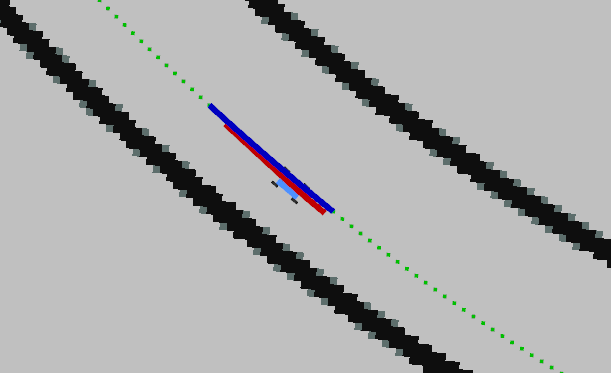
\includegraphics[scale=0.7]{images/mpc_viz.png}
    \caption{Visualizzazione dei ROS topic utilizzati per \textit{MPC}.}
    \label{fig:fig12} % etichetta utilizzata per riferisi all'immagine
\end{figure}
Per visualizzare l'algoritmo si creano e, infine, si pubblicano i marker che rappresentano:
\begin{itemize}
    \item i \textit{waypoints}, che rappresentano i punti di riferimento che il veicolo deve seguire;
    per mostrarli si utilizza un marker verde di tipo \verb|POINTS|.
    \item la \textit{traiettoria di riferimento}, ovvero la traiettoria ideale che il veicolo dovrebbe 
    seguire, mostrata mediante un marker blu di tipo \verb|LINE_STRIP|.
    \item il \textit{percorso predetto}, cioè la traiettoria che il veicolo seguirà in base agli input di 
    controllo attuali, mostrata con un marker rosso di tipo \verb|LINE_STRIP|.
\end{itemize}
Tuttavia, si specifica che per visualizzare i marker pubblicati è necessario aggiungere delle nuove 
schermate di tipologia \verb|Marker| su \verb|RViz|, per ciascuna delle tre visualizzazioni. 
Inoltre, bisogna configurare correttamente i \verb|topic| su cui si pubblicano i marker definiti, ad esempio, per i waypoints è stato scelto il nome ``\verb|/visualization_waypoints|''.
\chapter{Analisi dei risultati}
\label{chap:chap5}
In questo capitolo si presentano e analizzano i risultati ottenuti con 
l'algoritmo \textit{Model Predictive Control}. In particolare, sono state individuate
delle metriche specifiche per misurare i risultati dell'algoritmo, i quali sono stati 
poi confrontati tra i diversi metodi di controllo, soprattutto per quanto riguarda
i profili di guida di \textit{MPC} nelle due piste testate.
Successivamente, i risultati ottenuti sono stati analizzati e rappresentati graficamente 
attraverso dei notebook \textit{Jupyter}, in modo da visualizzare le peculiarità emerse dal 
lavoro svolto.

\section{Metriche usate}
\label{subs:metrics}
%\section{Confronto per i circuiti}
L'analisi dei risultati -- e il resto del lavoro -- è stata effettuata su 
Ubuntu 22.04 (kernel 6.8.0-45-generic), con un sistema avente 
come CPU un i5-12600K @ 4.9GHz e 32 GB di RAM DDR4 @ 3200 MHz.
Gli esperimenti condotti comprendono principalmente dei test sui tracciati 
di \textit{Spa} e \textit{Monza} per ciascun profilo di guida di \textit{MPC}. Ognuno di essi è stato
confrontato con \textit{Pure Pursuit}, che è stato sfruttato come metodo
\textit{baseline}. Inoltre, sono stati effettuati confronti tra i tre profilo di \textit{MPC}:
in questo caso, si è preso il profilo \textit{High Performance} come riferimento. 

Ciascuna configurazione del 
sistema è stata testata al fine di ottenere una valutazione complessiva delle diverse situazioni 
operative in cui l'algoritmo si è trovato ad agire.

Le metriche individuate per l'analisi delle performance del controllore 
comprendono~\cite{dighe2023kinematics}:
\begin{itemize}
    \item \textit{Lap time}, cioè la misurazione del tempo sul giro, che viene misurato da quando 
    l'auto supera il punto di partenza fino a quando lo raggiunge nuovamente.
    \item \textit{Errore di tracking}, detto anche \textit{Crosstrack Error}, cioè la distanza tra 
    la linea teorica e quella che viene realmente seguita dal veicolo in una specifica posizione  
    nella mappa. In più, si va a misurare la \textit{deviazione massima} \(d_\text{max}\) dalla linea di riferimento.
    \[ \text{Errore di Tracking} = d = \sqrt{(x_\text{actual} - x_\text{ref})^2 + (y_\text{actual} - y_\text{ref})^2}
    \]
    \item \textit{Deviazione standard campionaria} dell'errore di tracking.
    \[
    \sigma_d = \sqrt{\frac{1}{n-1} \sum_{i=1}^{n} (d_i - \mu)^2}
    \]
    %\item \textit{Mean Squared Error (MSE)}, corrispondente 
    %all'errore quadratico medio relativo al quadrato 
    %dell'errore di tracking.
    %\[ \text{MSE} = 
    %\frac{1}{n} \sum_{i=1}^{n} d_i^2
    %\]
    \item \textit{Root Mean Squared Error (RMSE)}, per valutare l'accuratezza del modello nel 
    seguire la traiettoria di riferimento. Infatti, misura la distanza tra il punto più vicino 
    della traiettoria di riferimento da seguire e la posizione effettiva del veicolo. Viene scelto 
    perché, essendo sensibile a valori grandi, esso penalizza maggiormente le deviazioni maggiori.
    \[ \text{RMSE} = 
    \sqrt{\frac{1}{n} \sum_{i=1}^{n} d_i^2}
    \]
    \item \textit{Consumo energetico}, misurato per ogni posizione dell'auto durante un giro.
    \[
    P = m a v = 3.74 \text{Kg} \ a v
    \]
\end{itemize}
Ognuna di queste metriche è stata misurata e calcolata per i circuiti usati, ovvero \textit{Spa} e \textit{Monza}, come detto in precedenza.

\subsection{Circuiti}
Dopo aver definito le metriche, per ciascun circuito sono stati raccolti i risultati ottenuti 
nelle tre configurazioni di \textit{MPC}.
Inoltre, come anticipato, è stato utilizzato \textit{Pure Pursuit} come 
\textit{baseline}~\cite{becker2023model} per confrontarlo con gli altri metodi di \textit{MPC}.

\begin{table}[H]
\centering
\begin{tabular}{|l|c|c|c|c|c|}
\hline
\multicolumn{6}{|c|}{\textbf{Circuito di Spa}} \\
\hline
\textbf{Metodo} & \textbf{Lap Time [s]} & $\bm{d}_\textbf{max} \textbf{[m]}$ & \textbf{RMSE [m]} & $\bm{\sigma}_\textbf{d}$ \textbf{[m]} & \textbf{Energia [W]} \\
\hline
\textit{Pure Pursuit} & \textit{85.1} & \textit{0.638} & \textit{0.211} & \textit{0.043} & \textit{6.352} \\
\hline
Safe MPC & 78.0 & 0.389 & 0.111 & 0.057 & 0.217 \\
Fast MPC & 75.2 & 0.380 & 0.115 & 0.06 & 0.547 \\
HP MPC & 68.5 & 0.518 & 0.088 & 0.044 & 2.748 \\
\hline
\multicolumn{6}{|c|}{\textbf{Circuito di Monza}} \\
\hline
%\textbf{Metodo} & \textbf{Lap Time} & $\bm{d}_\textbf{max}$ & \textbf{RMSE} & $\bm{\sigma}_\textbf{d}$ & \textbf{Energia} \\
%\hline
\textit{Pure Pursuit} & \textit{57.4} & \textit{0.679} & \textit{0.21} & \textit{0.045} & \textit{6.944} \\
\hline
Safe MPC & 52.4 & 0.244 & 0.087 & 0.047 & 0.841 \\
Fast MPC & 50.6 & 0.299 & 0.092 & 0.051 & 0.706 \\
HP MPC & 49.6 & 0.261 & 0.083 & 0.044 & 1.156 \\
\hline
\end{tabular}
\caption{Confronto dei metodi di \textit{MPC} con \textit{Pure Pursuit} come baseline.}
\label{tab:spa_monza_mpc_comparison}
\end{table}
Dai risultati ottenuti e indicati nella Tabella~\ref{tab:spa_monza_mpc_comparison},
emergono diversi punti chiave da considerare per le due piste:
\begin{enumerate}
    \item \textit{Lap Time} -- I diversi profili di \textit{MPC} superano 
    nettamente \textit{Pure Pursuit}, con \textit{High Performance MPC} che 
    risulta essere il più veloce in entrambi i circuiti. Questi risultati 
    suggeriscono che l’ottimizzazione svolta con \textit{MPC} permette di 
    migliorare significativamente anche la velocità media nel circuito, come
    si può notare nella Tabella~\ref{tab:spa_under_over_performance}.
    \item \textit{Deviazione massima dalla traiettoria ideale} -- \textit{Safe MPC} è il profilo 
    con la deviazione massima inferiore su \textit{Monza}, mentre su \textit{Spa} è invece \textit{Fast MPC}.
    Si osserva come \textit{Pure Pursuit} si discosta maggiormente dalla traiettoria ideale in entrambi i circuiti.
    \item \textit{RMSE} -- \textit{HP MPC} gode di valori di \textit{RMSE} inferiori per entrambe 
    le piste. Esso quindi garantisce una maggior precisione nel seguire la traiettoria.
    Infatti, si rileva che \textit{Pure Pursuit} ha un errore superiore rispetto a 
    \textit{HP MPC} di circa il $153 \%$ per \textit{Monza} e di circa il $140 \%$ per \textit{Spa}. 
    Inoltre, il profilo \textit{Safe} ha valori inferiori rispetto al \textit{Fast}. 
    \item \textit{Deviazione standard dell'errore di tracking} -- 
    \textit{Fast MPC} tende ad avere più variabilità nella traiettoria 
    seguita, seguito in ordine dai profili \textit{Safe} e \textit{HP}; 
    d'altro canto, \textit{Pure Pursuit} ha una variabilità della 
    traiettoria ridotta, molto simile a quella di \textit{HP MPC}.
    \item \textit{Consumo energetico} -- \textit{HP MPC} tende a consumare
    in media più energia per poter ottenere prestazioni migliori, tuttavia
    \textit{Pure Pursuit} consuma molto di più, senza però offrire le stesse performance e gli stessi vantaggi di \textit{MPC}.
\end{enumerate}
Infine, la Tabella~\ref{tab:spa_under_over_performance} riporta i dati relativi 
alle velocità ottenute con ciascun metodo di controllo. Queste vengono confrontate coi 
valori teorici segnati nel dataset per ciascun waypoint. 
Dai risultati nei profili di \textit{MPC} si rileva che, se per \textit{Monza}
non si osserva un superamento delle prestazioni rispetto alle velocità teoriche 
generate dal \textit{planner}, per \textit{Spa} si ottiene sempre un miglioramento,
eccetto che per \textit{Safe MPC}.
%Infatti, se per \textit{Pure Pursuit} essa è di 7.56 m/s per Spa (8.82 
%m/s per Monza), per \textit{Safe MPC} vale 8.07 m/s (9.25 m/s per 
%Monza), per \textit{Fast MPC} vale 8.34 m/s (9.72 m/s per Monza) e per 
%\textit{HP MPC} invece 8.6 m/s (9.77 m/s per Monza).
\begin{table}[H]
\centering
\begin{tabular}{|l|c|c|c|}
\hline
\multicolumn{4}{|c|}{\textbf{Velocità per il circuito di Spa}} \\
\hline
\textbf{Metodo} & \textbf{Media [m/s]} & \textbf{Underperf. [\%]} & \textbf{Overperf. [\%]} \\
\hline
\textit{Pure Pursuit} & \textit{7.56} & \textit{93.49} & \textit{6.51} \\
\hline
Safe MPC & 8.07 & 64.22 & 35.78 \\
Fast MPC & 8.34 & 45.67 & 54.33 \\
HP MPC & 8.6 & 38.41 & 61.59 \\
\hline
\multicolumn{4}{|c|}{\textbf{Velocità per il circuito di Monza}} \\
\hline
%\textbf{Metodo} & \textbf{Valore medio} & \textbf{Underperformance} & \textbf{Overperformance} \\
%\hline
\textit{Pure Pursuit} & \textit{8.82} & \textit{96.49} & \textit{3.51} \\
\hline
Safe MPC & 9.25 & 66.55 & 33.45 \\
Fast MPC & 9.72 & 56.79 & 43.21 \\
HP MPC & 9.77 & 54.18 & 45.82 \\
\hline
\end{tabular}
\caption{Confronto dei rendimenti rispetto alla velocità di riferimento per
i circuiti di \textit{Spa} e \textit{Monza}.}
\label{tab:spa_under_over_performance}
\end{table}
Ricapitolando, le configurazioni di \textit{MPC}, rispetto a \textit{Pure Pursuit}, non solo 
migliorano la precisione nel tracking della traiettoria e i tempi di percorrenza del circuito, ma 
evidenziano anche un'evidente efficienza energetica superiore, considerando anche la scala ridotta del veicolo. 
In particolare, il profilo \textit{High Performance MPC} emerge come il metodo più 
\textit{robusto}, con prestazioni considerevoli e consumi energetici discreti.
%\section{Profili}
%\subsection{Realistico}
%\subsection{Veloce}
%\subsection{Performante}
\section{Visualizzazione dei risultati}
In questa sezione vengono presentati graficamente i risultati relativi ad altri
aspetti del controllo del veicolo applicato al \textit{path tracking}.
I risultati sono visualizzati sia per i tre profili di \textit{MPC}, che vengono confrontati 
tra loro, sia in relazione al \textit{Pure Pursuit}. Inoltre, in alcuni grafici essi vengono 
mostrati anche rispetto ai valori teorici della \textit{raceline}, che viene presa come riferimento per i dati teorici.
\subsection{Lap time}
I tempi di percorrenza su un giro (\textit{lap time}) sono stati misurati a partire
dal secondo, così da consentire al veicolo di stabilizzarsi dopo la partenza.
Si è scelto di non misurare oltre anche perché, dopo il secondo giro, le variazioni nei tempi registrati risultano trascurabili.

\begin{figure}[H]
    \centering
    \begin{subfigure}[b]{0.49\textwidth}
        \centering
        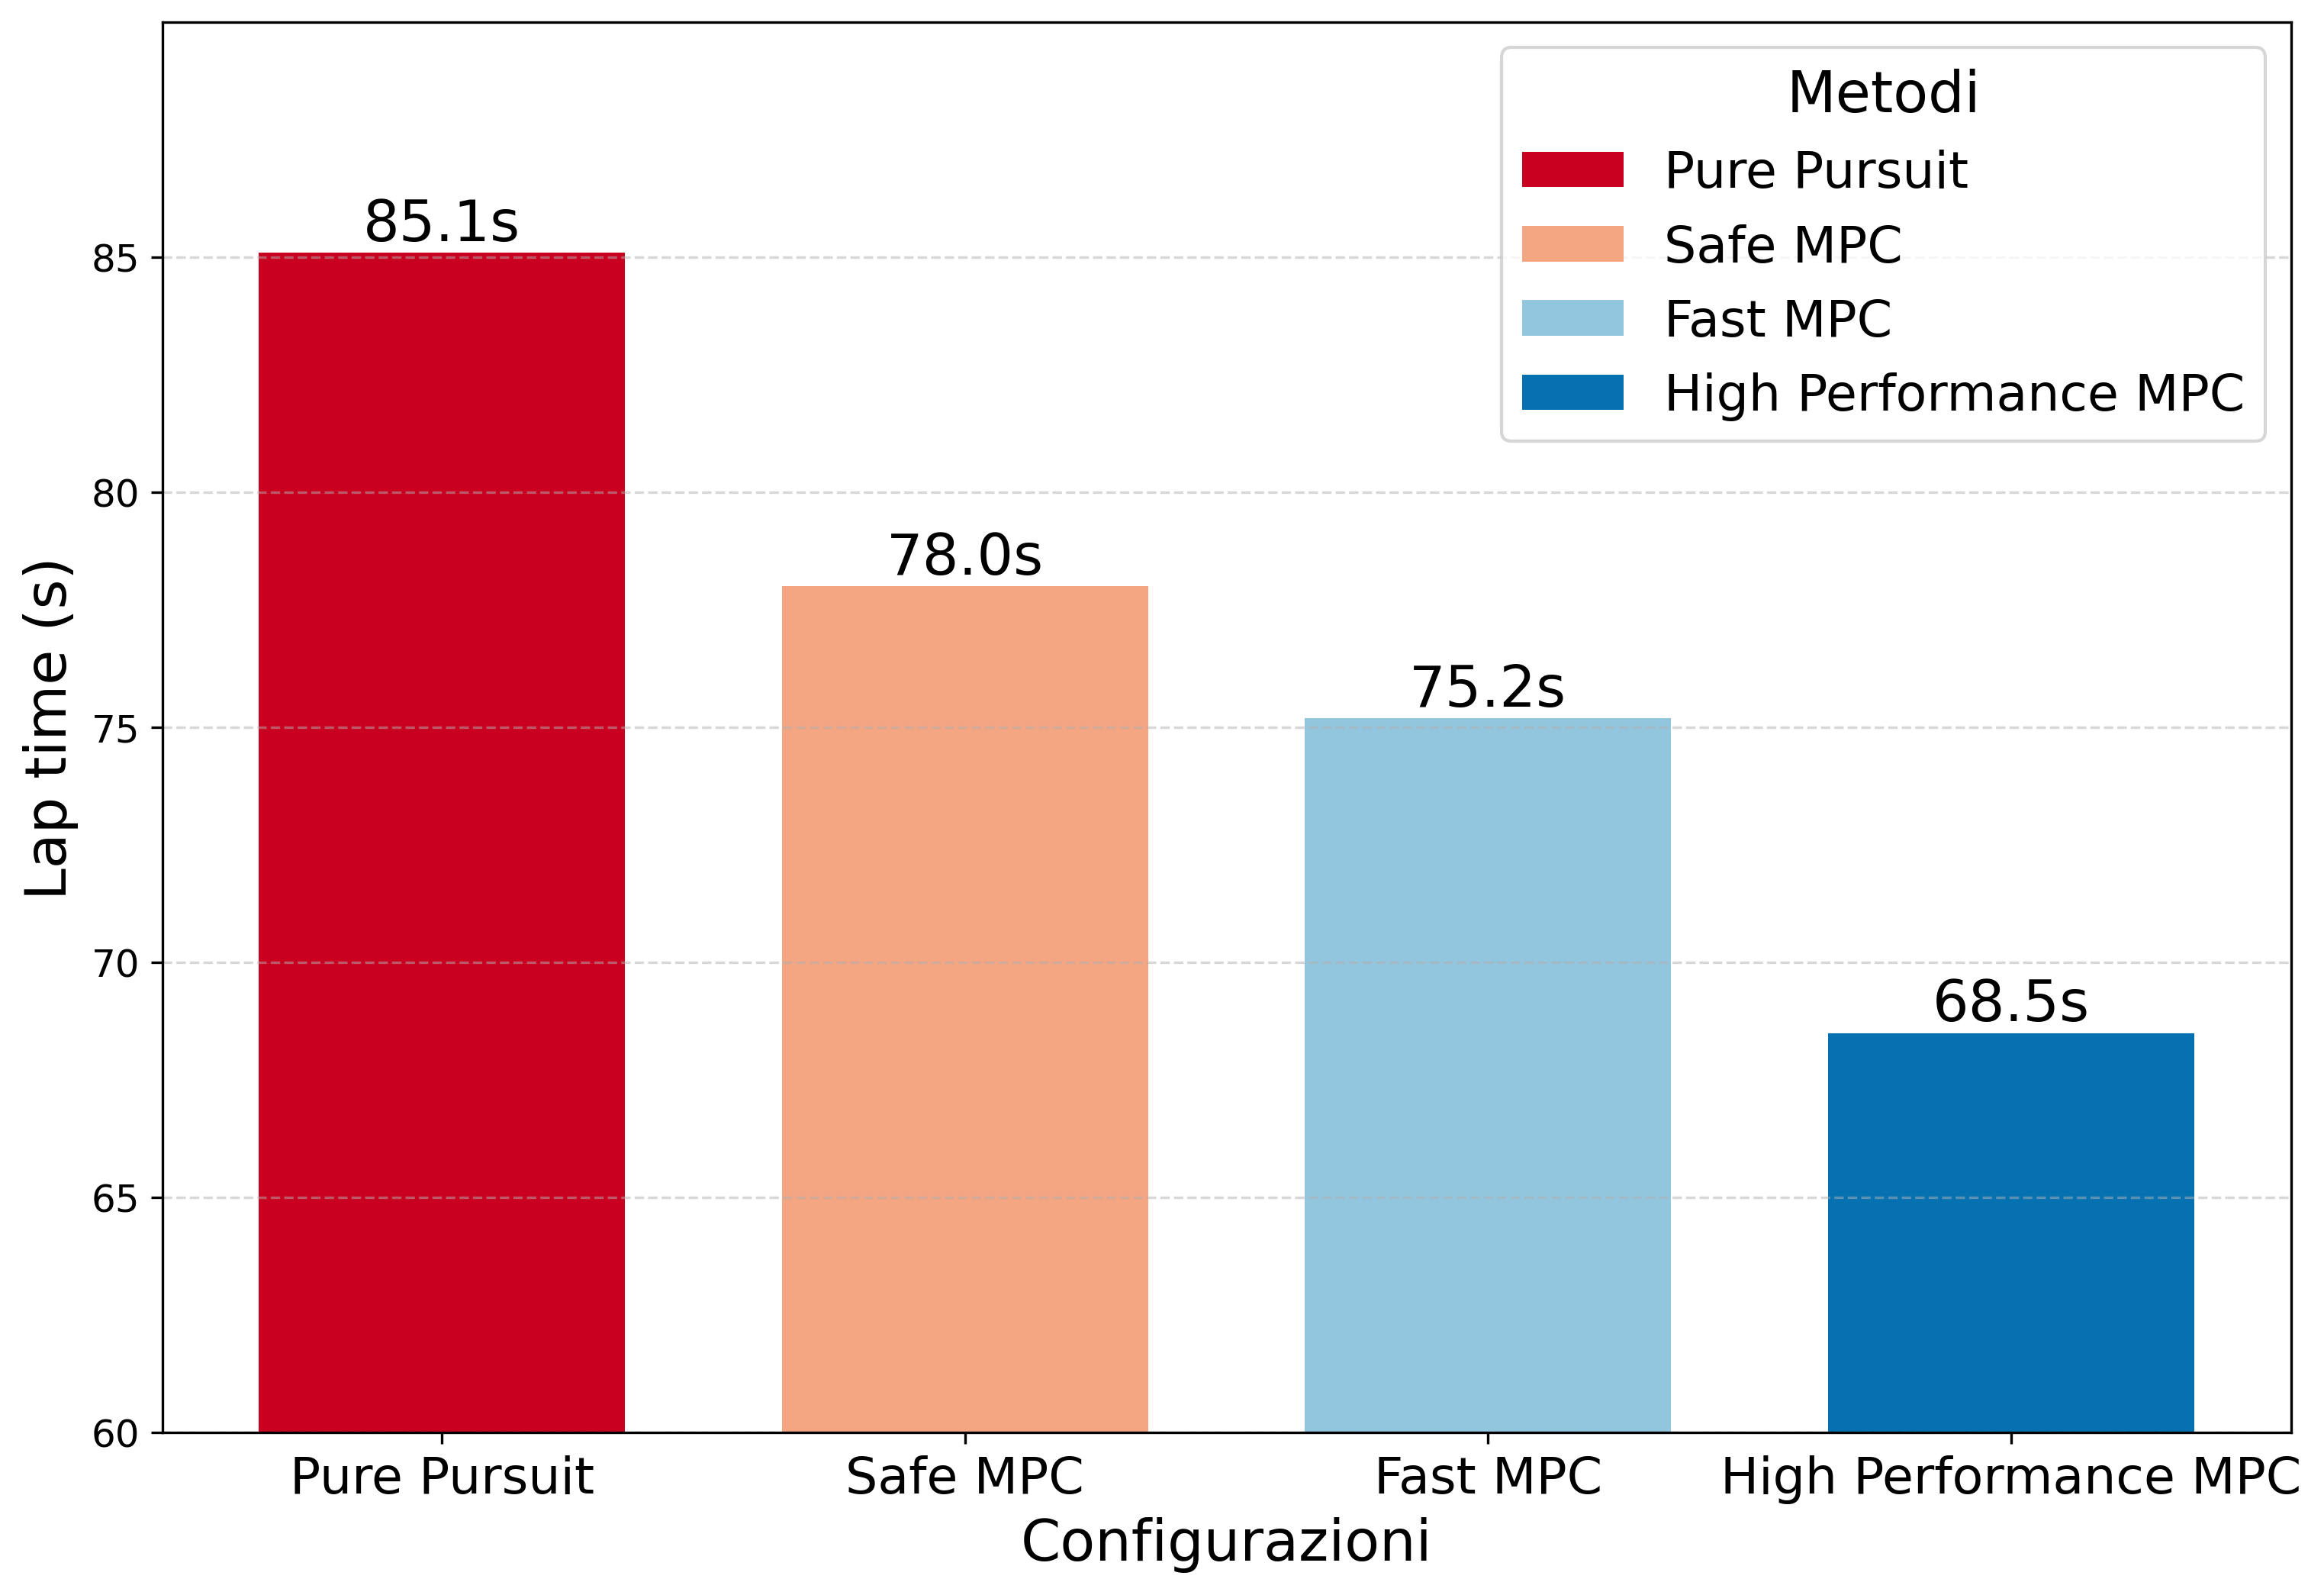
\includegraphics[width=\textwidth]{images/spa_lap_time_comparisons.png} 
        \caption{\textit{Spa}}
        \label{fig:laptime_spa}
    \end{subfigure}
    %\vfill
    \begin{subfigure}[b]{0.49\textwidth}
        \centering
        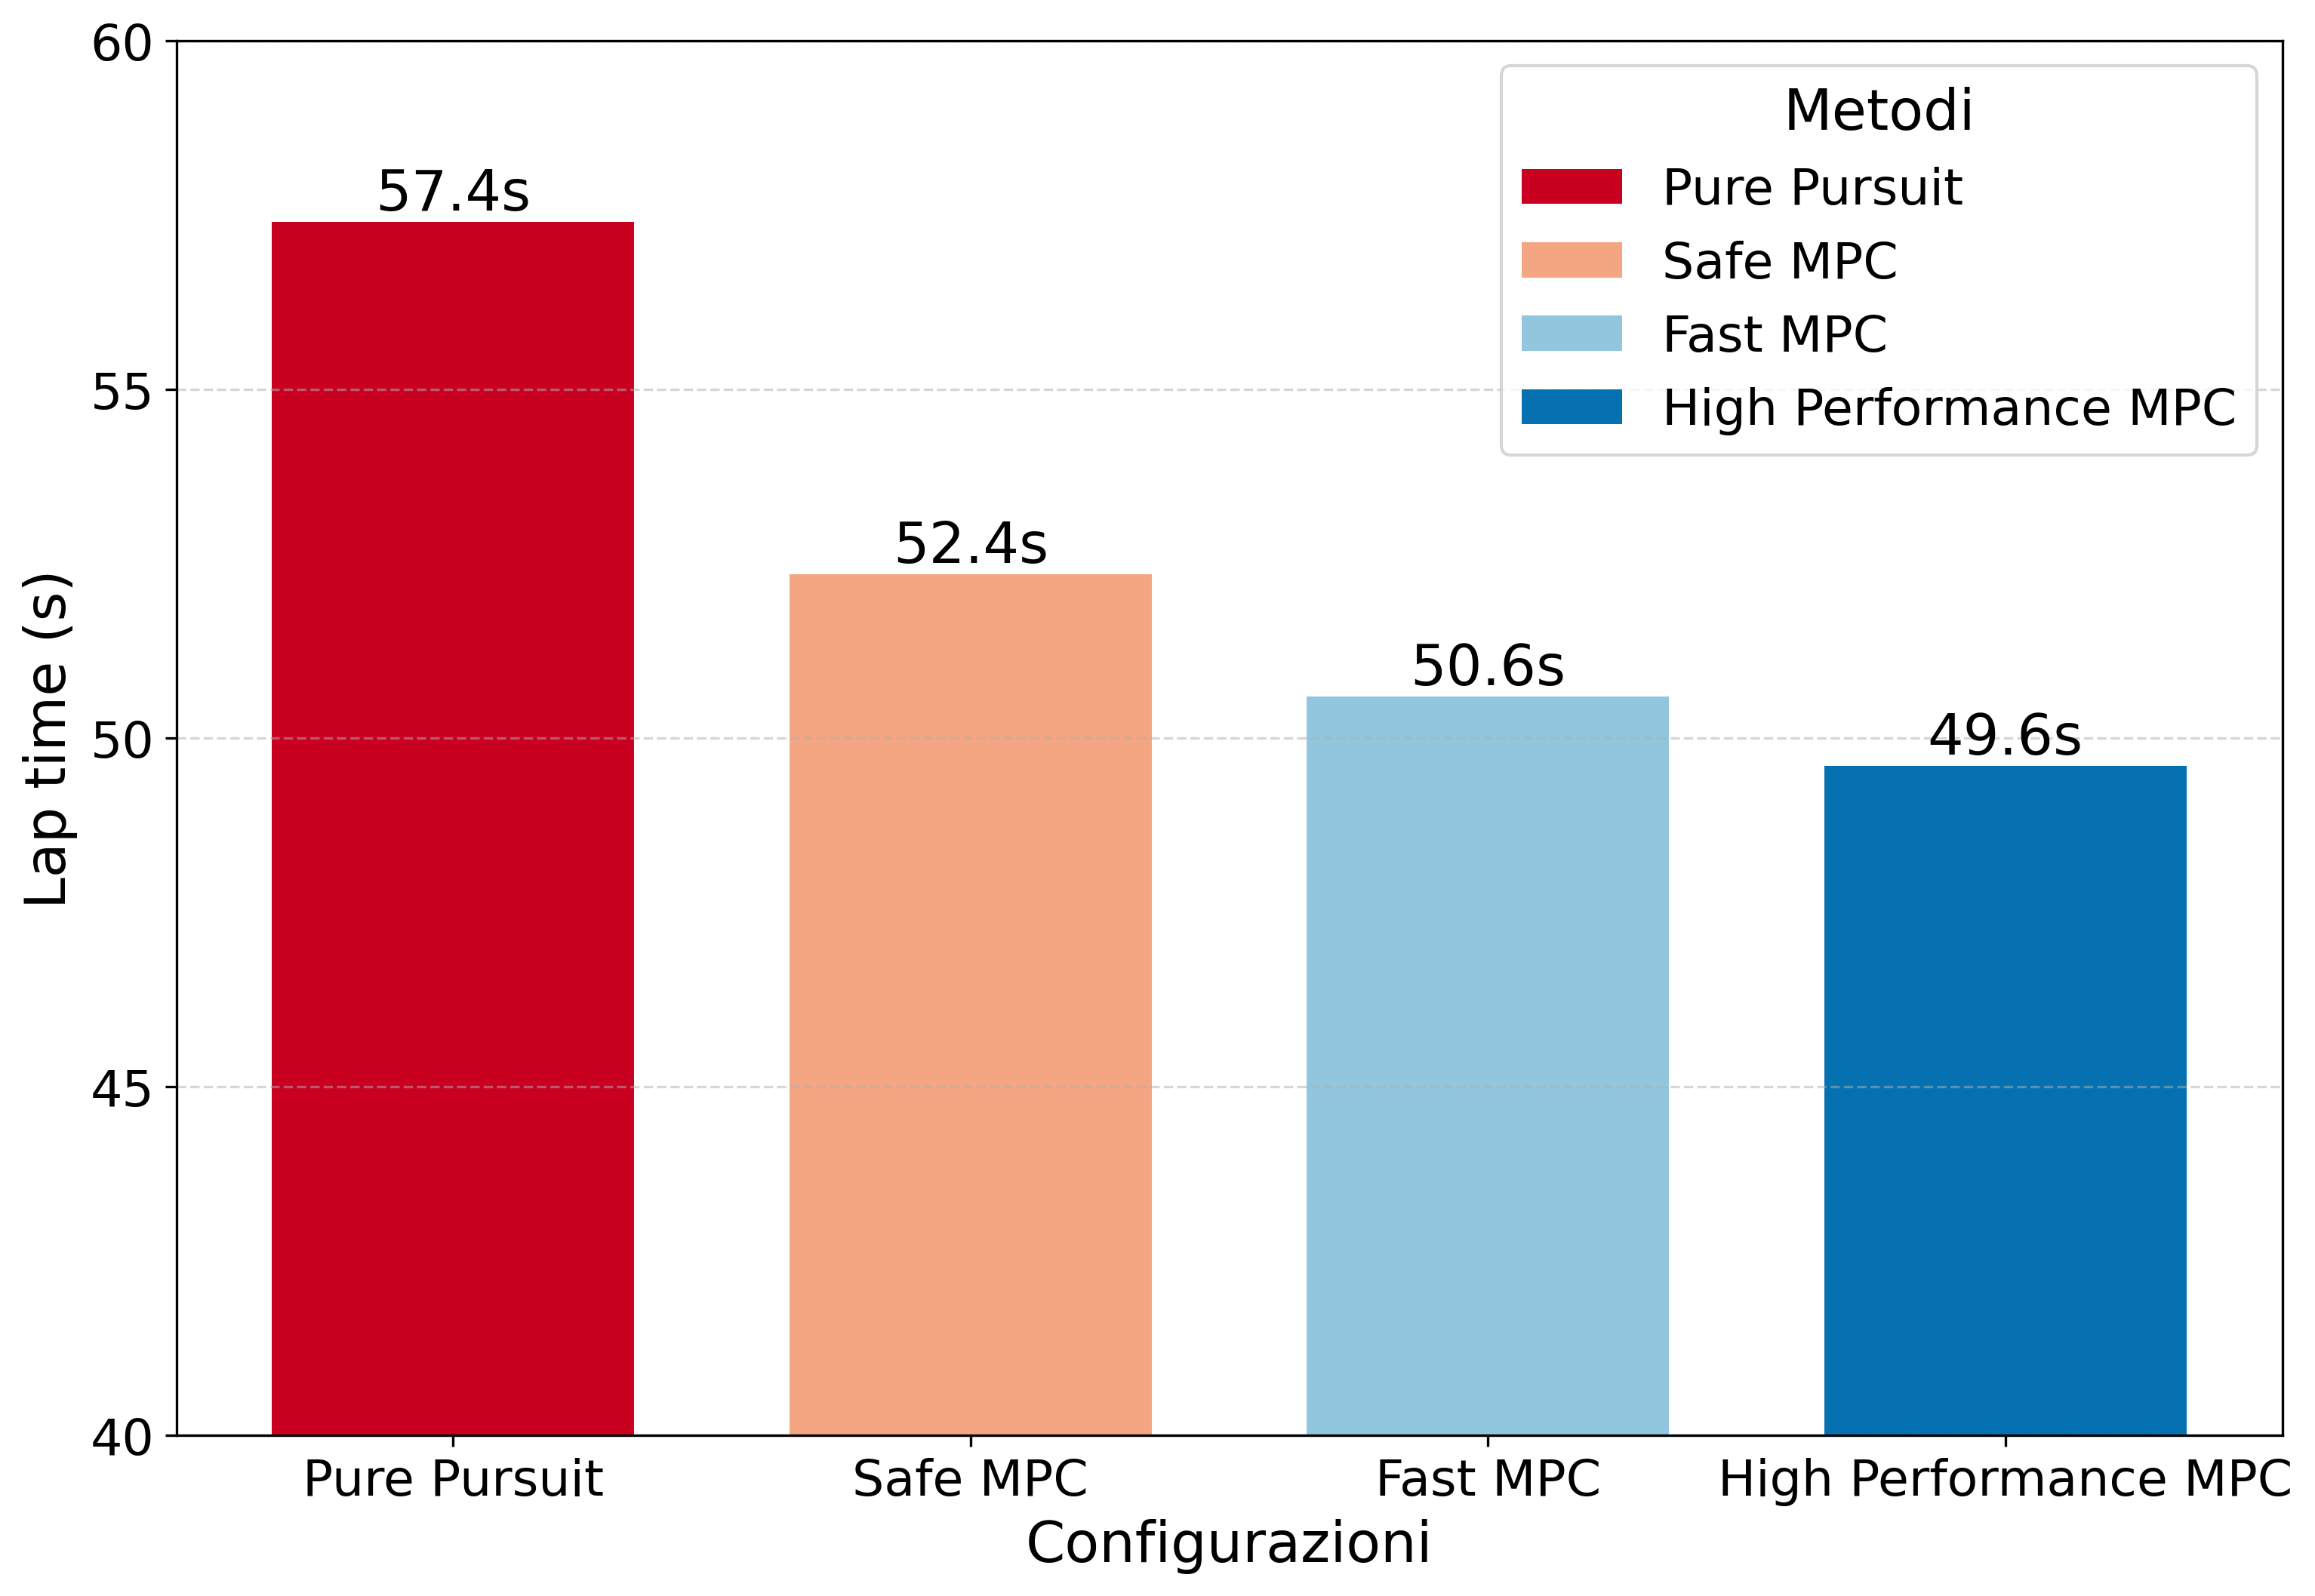
\includegraphics[width=\textwidth]{images/monza_lap_time_comparisons.png}
        \caption{\textit{Monza}}
        \label{fig:laptime_monza}
    \end{subfigure}
    \caption{Lap time per ogni metodo di controllo misurato.}
    \label{fig:fig13} % etichetta utilizzata per riferisi all'immagine
\end{figure}
Si possono osservare in Fig.~\ref{fig:fig13} i tempi per \textit{Pure Pursuit}
e per ciascuna configurazione di \textit{Model Predictive Control}.
Essi rispecchiano le aspettative: il metodo col \textit{lap time} inferiore risulta essere 
\textit{High Performance MPC}, seguito dai metodi \textit{Fast} e \textit{Safe}. 
Invece, \textit{Pure Pursuit} richiede più tempo per completare un giro e, provando a farlo 
correre ripetutamente, tende ad andare a sbattere con più frequenza per via della semplicità di 
questo metodo di controllo \textit{reattivo} e \textit{geometrico}.

\subsection{Traiettorie}
Per visualizzare le traiettorie, essendo molto ravvicinate tra loro, si utilizzano degli
\textit{zoom} su delle zone specifiche del tracciato, ovvero un \textit{rettilineo} e 
alcune tipologie di curve che sono molto comuni nelle piste di \textit{Formula 1}:
\begin{enumerate}
    \item \textit{Chicane} -- Si tratta di una curva seguita da un'altra 
    curva nella direzione opposta che viene introdotta in un tratto 
    rettilineo di una pista per rallentare la velocità dei veicoli. 
    Può essere utilizzata per testare quanta velocità il veicolo riesce a portare verso 
    l'\textit{apex} (centro curva) -- il punto più interno seguito in una curva -- in entrambe le 
    curve, e con quanto anticipo ciò consente al sistema di accelerare in uscita dalla curva.
    \item \textit{Tornante} -- È una svolta di 180 gradi che permette di verificare il modo in cui 
    il sistema raggiunge l'\textit{apex} e, soprattutto, come entra ed esce dalle curve.
\end{enumerate}
Il circuito di \textit{Spa} presenta delle curve \textit{chicane} e un 
\textit{tornante}. Come visibile dalla Fig.~\ref{fig:fig14}, le traiettorie 
relative ai profili di \textit{MPC} sono più uniformi, poiché l'algoritmo ottimizza
sempre \textit{``online''}, e tendono a tagliare prima nelle curve rispetto al riferimento della 
\textit{raceline}. Le differenze tra i profili di \textit{MPC} sono dovute prettamente ai diversi
valori dell'orizzonte temporale e delle matrici di pesi, concetti già discussi nel 
Capitolo~\ref{chap:chap3}, da un punto di vista teorico, e nel Capitolo~\ref{chap:chap4} a livello implementativo.

A differenza di \textit{MPC}, \textit{Pure Pursuit} ha un andamento 
più variabile, poiché tende a correggere l'angolo di sterzata con elevata frequenza, per seguire
il più possibile i waypoints della \textit{raceline} a cui fa riferimento. 
Quanto descritto lo si può notare specialmente nella curva a gomito della 
Fig.~\ref{fig:curva_spa}, nella quale \textit{HP MPC} taglia molto in anticipo rispetto a tutti gli altri.

\begin{figure}[H]
    \centering
    \begin{subfigure}[b]{0.49\textwidth}
        \centering
        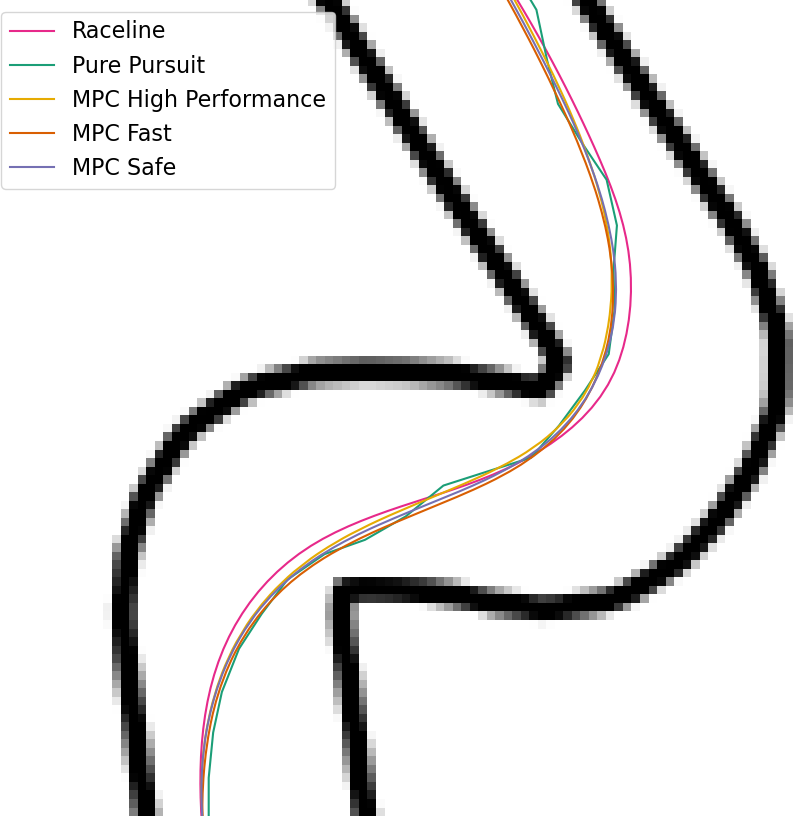
\includegraphics[width=\textwidth]{images/spa_traj_comparison_chicane.png} 
        \caption{Chicane}
        \label{fig:chic_spa}
    \end{subfigure}
    \hfill
    \begin{subfigure}{0.49\textwidth}
        \centering
        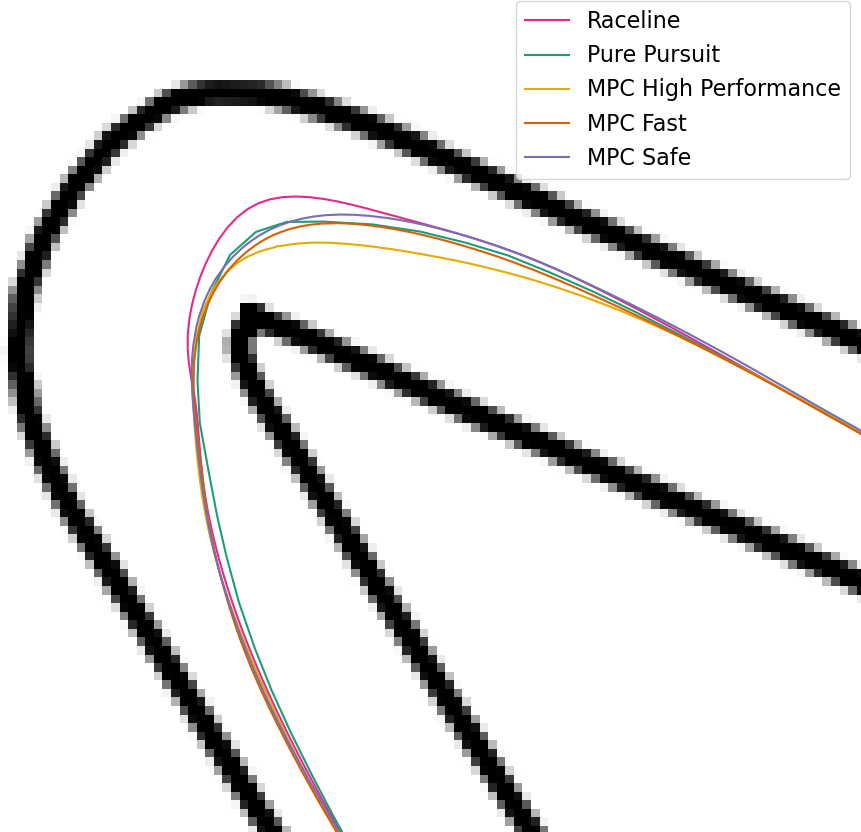
\includegraphics[width=\textwidth]{images/spa_traj_comparison_curva.png}
        \caption{Curva a gomito}
        \label{fig:curva_spa}
    \end{subfigure}
    \begin{subfigure}[b]{0.50\textwidth}
        \centering
        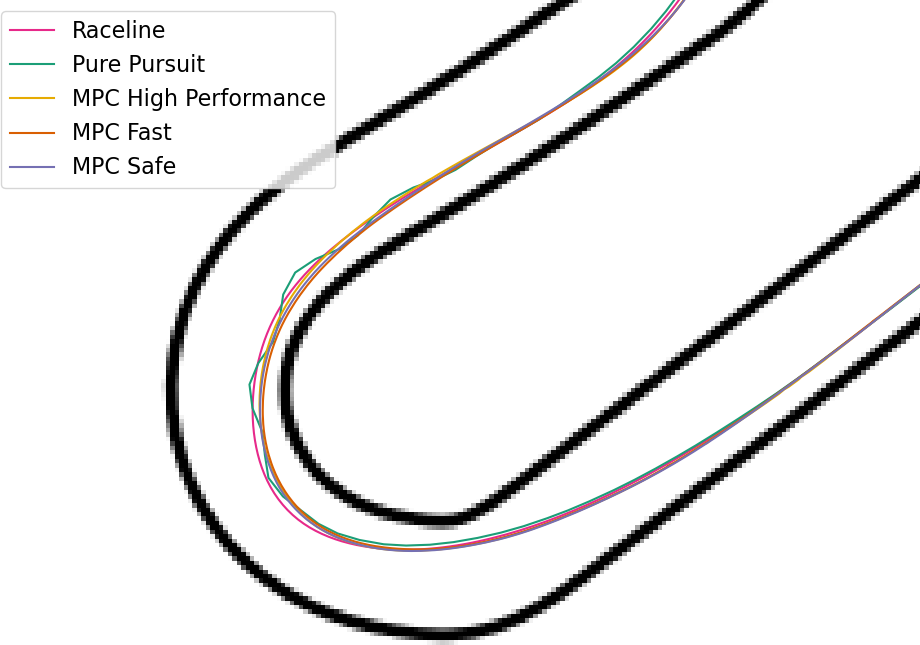
\includegraphics[width=\textwidth]{images/spa_traj_comparison_tornante.png}
        \caption{Tornante}
        \label{fig:torn_spa}
    \end{subfigure}
    \caption{Diversi tipi di curve su \textit{Spa}.}
    \label{fig:fig14} % etichetta utilizzata per riferisi all'immagine
\end{figure}

Si può notare in Fig.~\ref{fig:fig15} un comportamento simile anche per il circuito di Monza, 
composto prettamente da chicane e da rettilinei. Questi ultimi sono visualizzati per entrambe
le piste nella Fig.~\ref{fig:fig16}, in modo da evidenziare la vicinanza di tutte le traiettorie, 
che risultano di fatto sovrapposte.

\begin{figure}[H]
    \centering
    \begin{subfigure}[b]{0.49\textwidth}
        \centering
        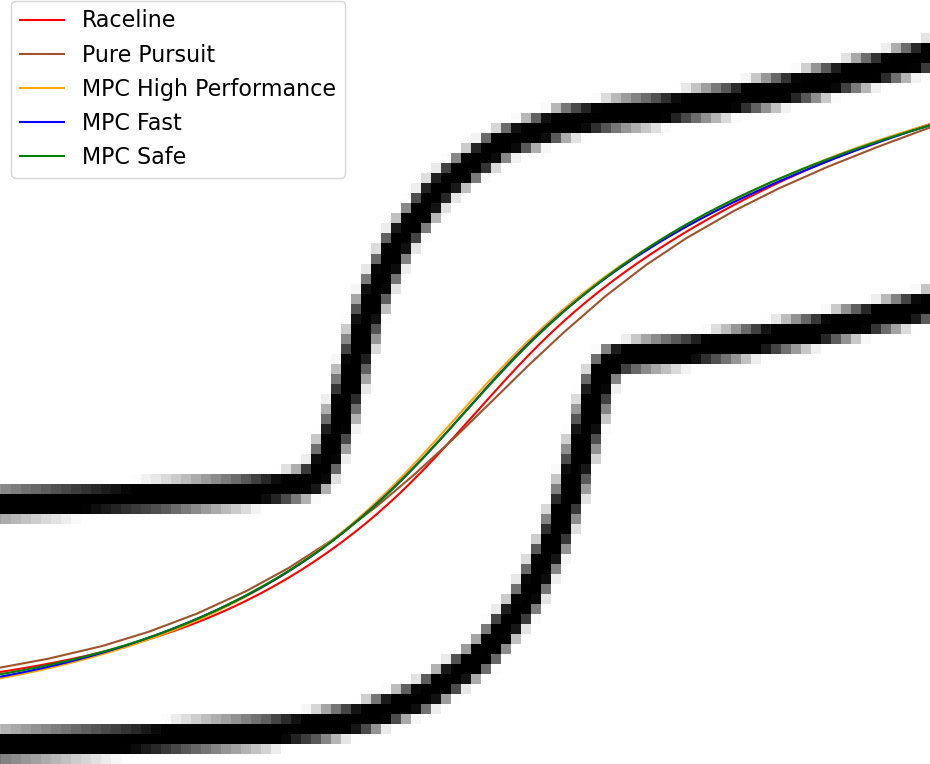
\includegraphics[width=\textwidth]{images/monza_traj_comparison_chicane.png} 
        \caption{Prima Chicane}
        \label{fig:chic_monza}
    \end{subfigure}
    \hfill
    \begin{subfigure}[b]{0.49\textwidth}
        \centering
        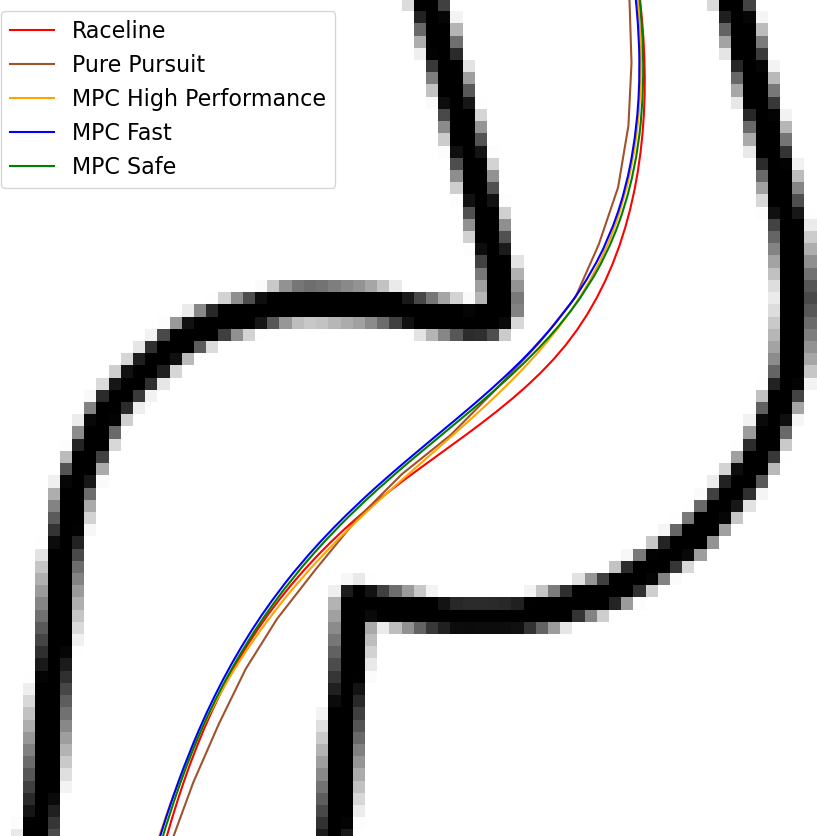
\includegraphics[width=\textwidth]{images/monza_traj_comparison_chicane2.png}
        \caption{Seconda Chicane}
        \label{fig:chic2_monza}
    \end{subfigure}
    \caption{Curve su \textit{Monza}.}
    \label{fig:fig15} % etichetta utilizzata per riferisi all'immagine
\end{figure}
\begin{figure}[H]
    \centering
    \begin{subfigure}[b]{0.49\textwidth}
        \centering
        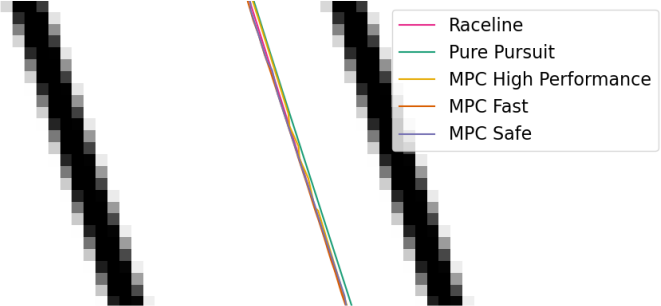
\includegraphics[width=\textwidth]{images/spa_trajectory_comparison_straight.png} 
        \caption{\textit{Spa}}
        \label{fig:str_spa}
    \end{subfigure}
    \hfill
    \begin{subfigure}[b]{0.49\textwidth}
        \centering
        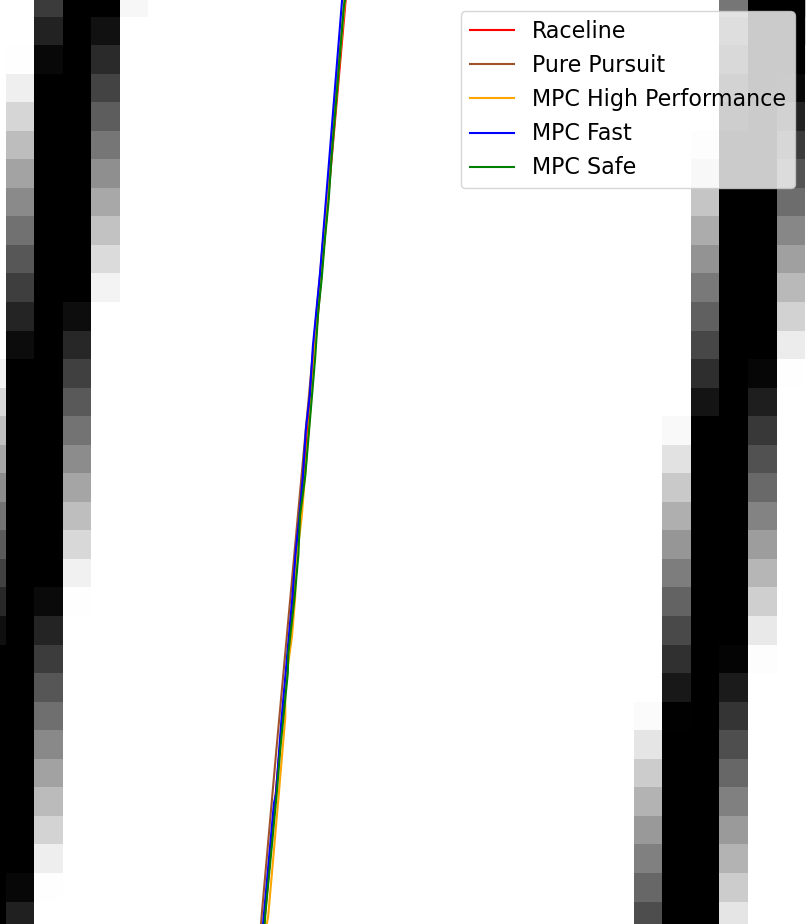
\includegraphics[width=0.8\textwidth]{images/monza_trajectory_comparison_straight.png}
        \caption{\textit{Monza}}
        \label{fig:str_monza}
    \end{subfigure}
    \caption{Rettilinei su \textit{Monza} e \textit{Spa}.}
    \label{fig:fig16} % etichetta utilizzata per riferisi all'immagine
\end{figure}

%    %\centering
%    %\includegraphics[scale=0.4]{images/%monza_mpc_safe_crosstrack_error.png}\hspace{0.02cm}
%    \includegraphics[scale=0.4]{images/monza_mpc_fast_crosstrack_error.png}


\subsection{Crosstrack Error}
Nella sezione~\ref{subs:metrics}, relativa alle metriche, è stato introdotto il 
\textit{Crosstrack Error}, detto anche errore di tracking. Tuttavia, questo dato è stato usato
esclusivamente per mostrare la \textit{deviazione massima} e, soprattutto, per calcolare l'\textit{RMSE}, in 
modo da avere una misura accurata che indica di quanto si discosta in media l'errore di tracking 
dallo zero, cioè il caso con valore teorico e valore corrente identici. 
Si vuole però dare anche un'idea visiva dell'evoluzione dell'errore di tracking, sempre attraverso la realizzazione di un grafico. 
Nella Fig.~\ref{fig:fig17} viene mostrato, per entrambe le piste, l'errore di tracking generato 
dal \textit{Pure Pursuit} che, come confermato dall'RMSE, ha valori mediamente superiori. 
Pertanto, questo metodo è stato utilizzato come \textit{baseline} anche per la scala cromatica in 
ogni grafico inerente a questa metrica. Si segnala che il triangolo indica la posizione di partenza del giro.

\begin{figure}[H]
    \centering
    \begin{subfigure}[b]{0.49\textwidth}
        \centering
        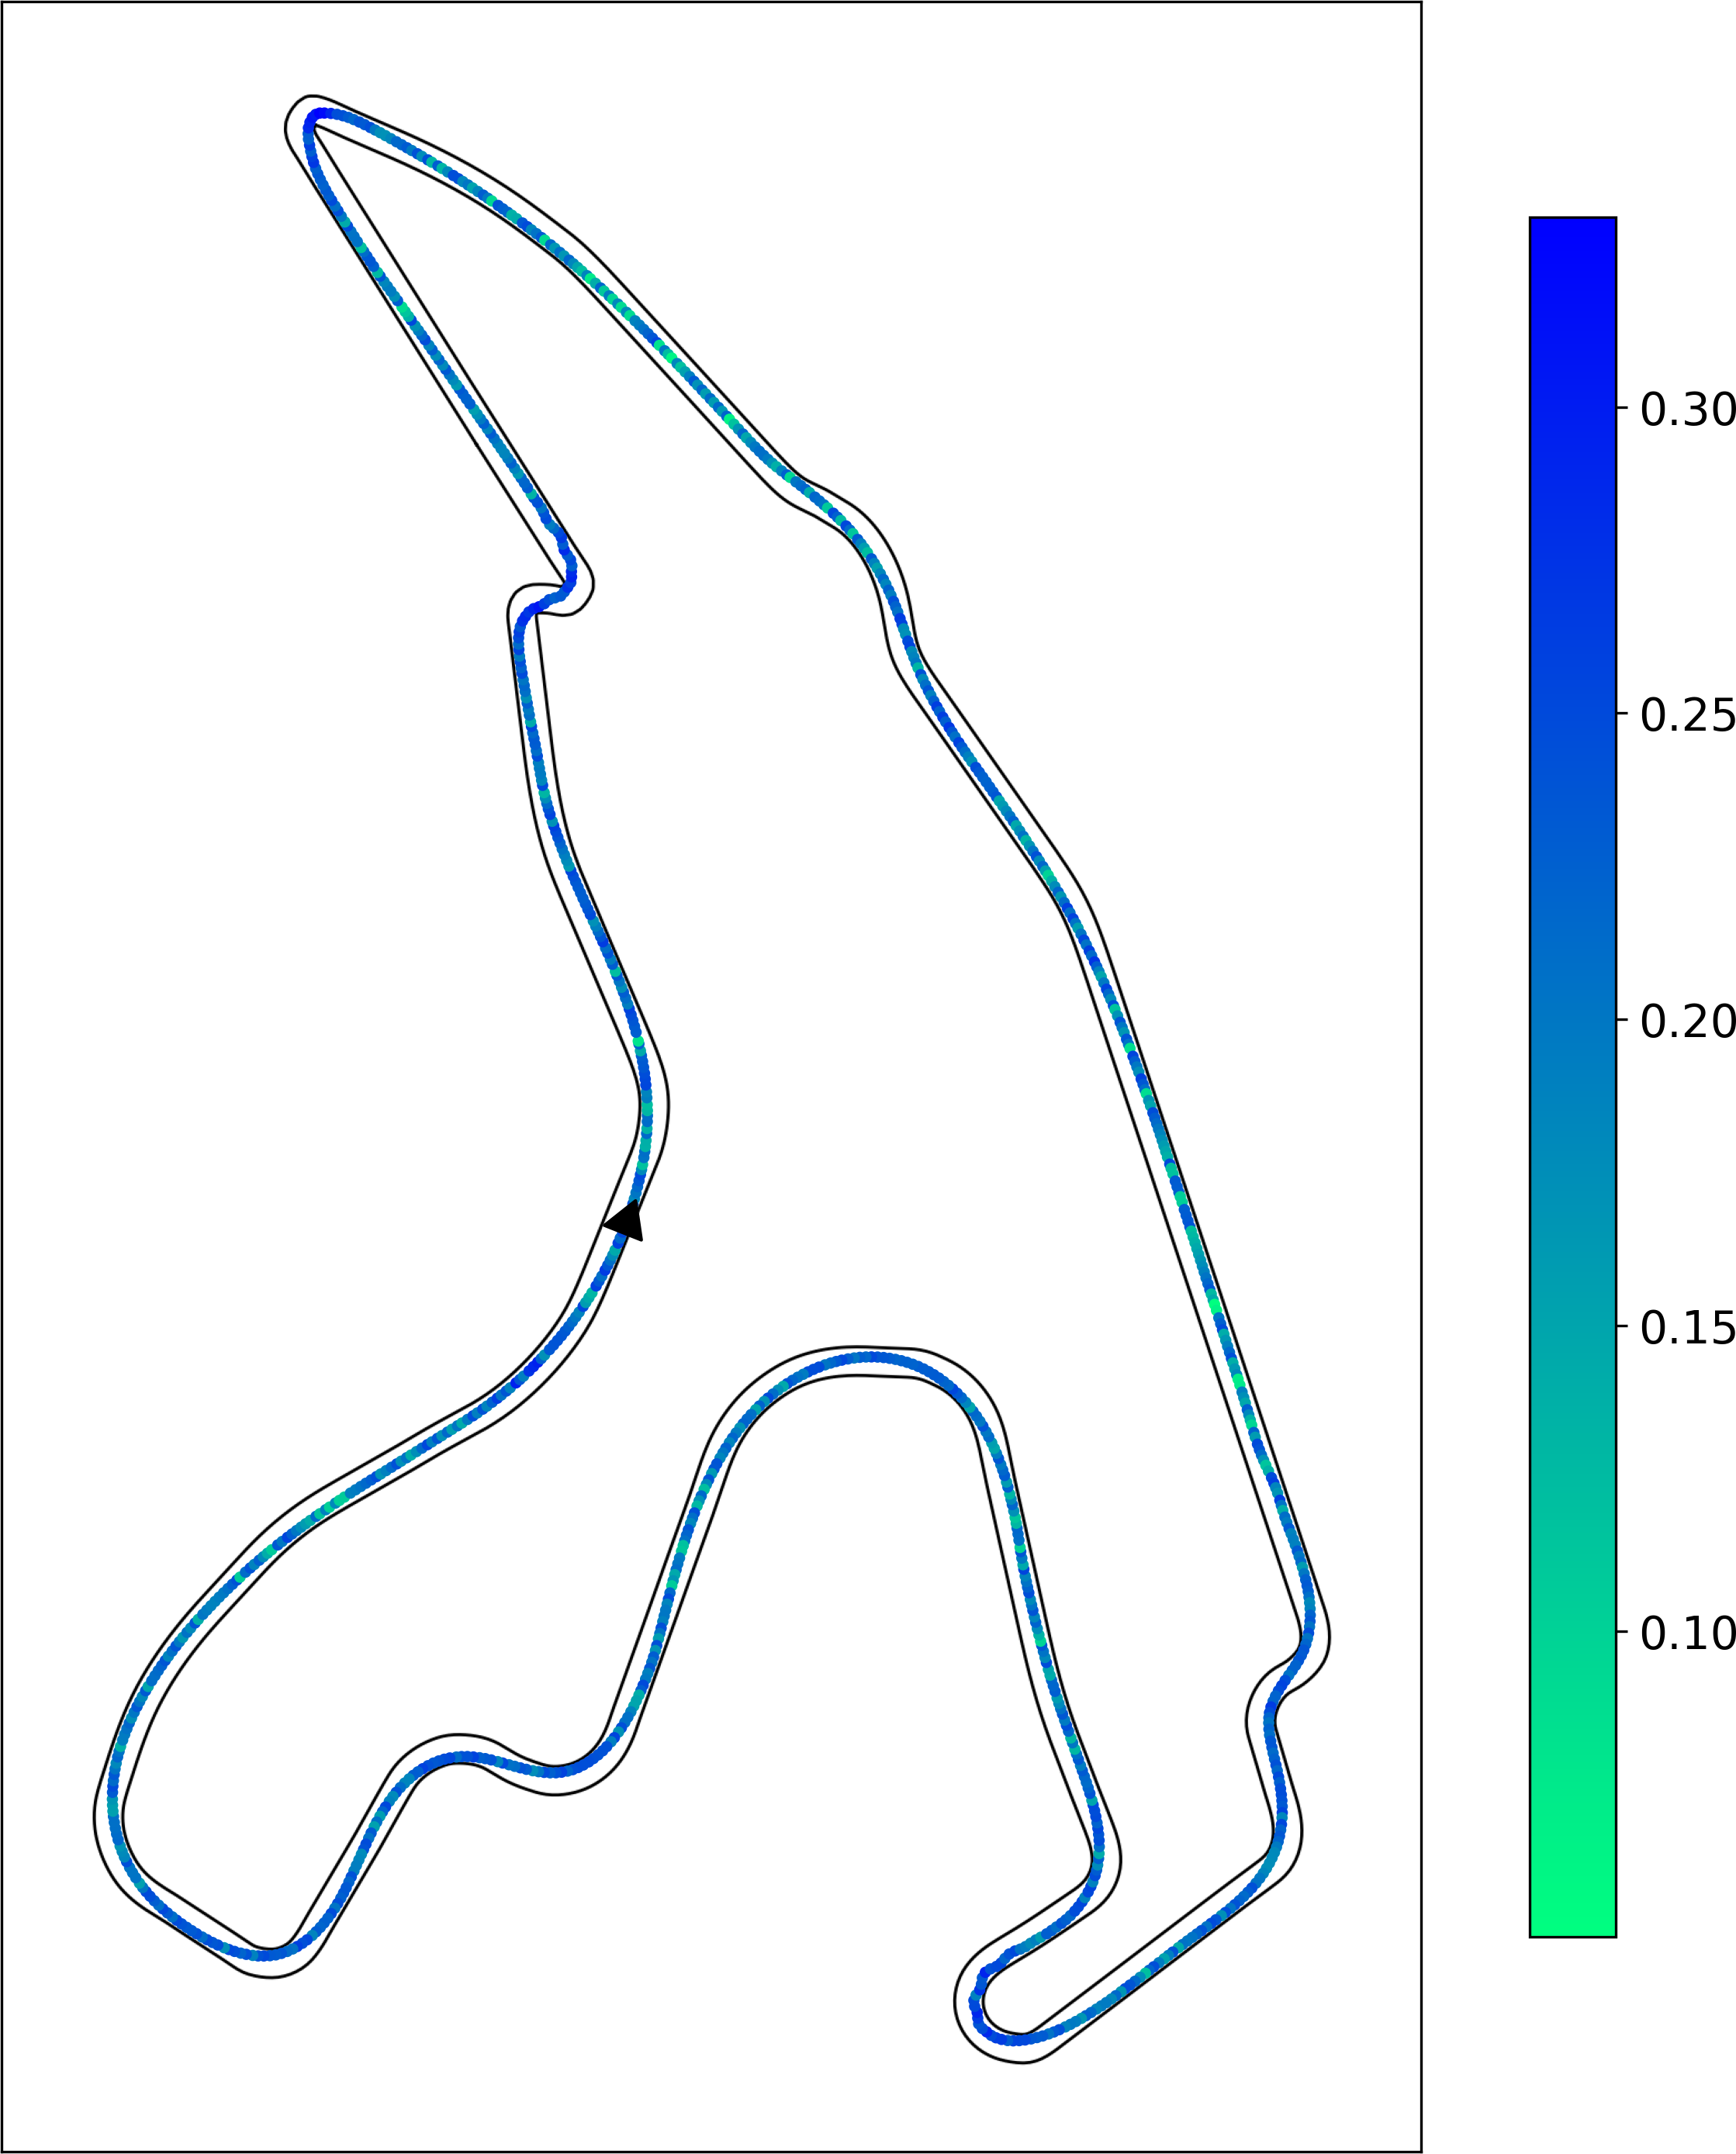
\includegraphics[width=0.75\textwidth]{images/spa_pp_crosstrack.png} 
        \caption{\textit{Spa}}
        \label{fig:tracking_pp_spa}
    \end{subfigure}
    %\hfill
    \begin{subfigure}[b]{0.469\textwidth}
        \centering
        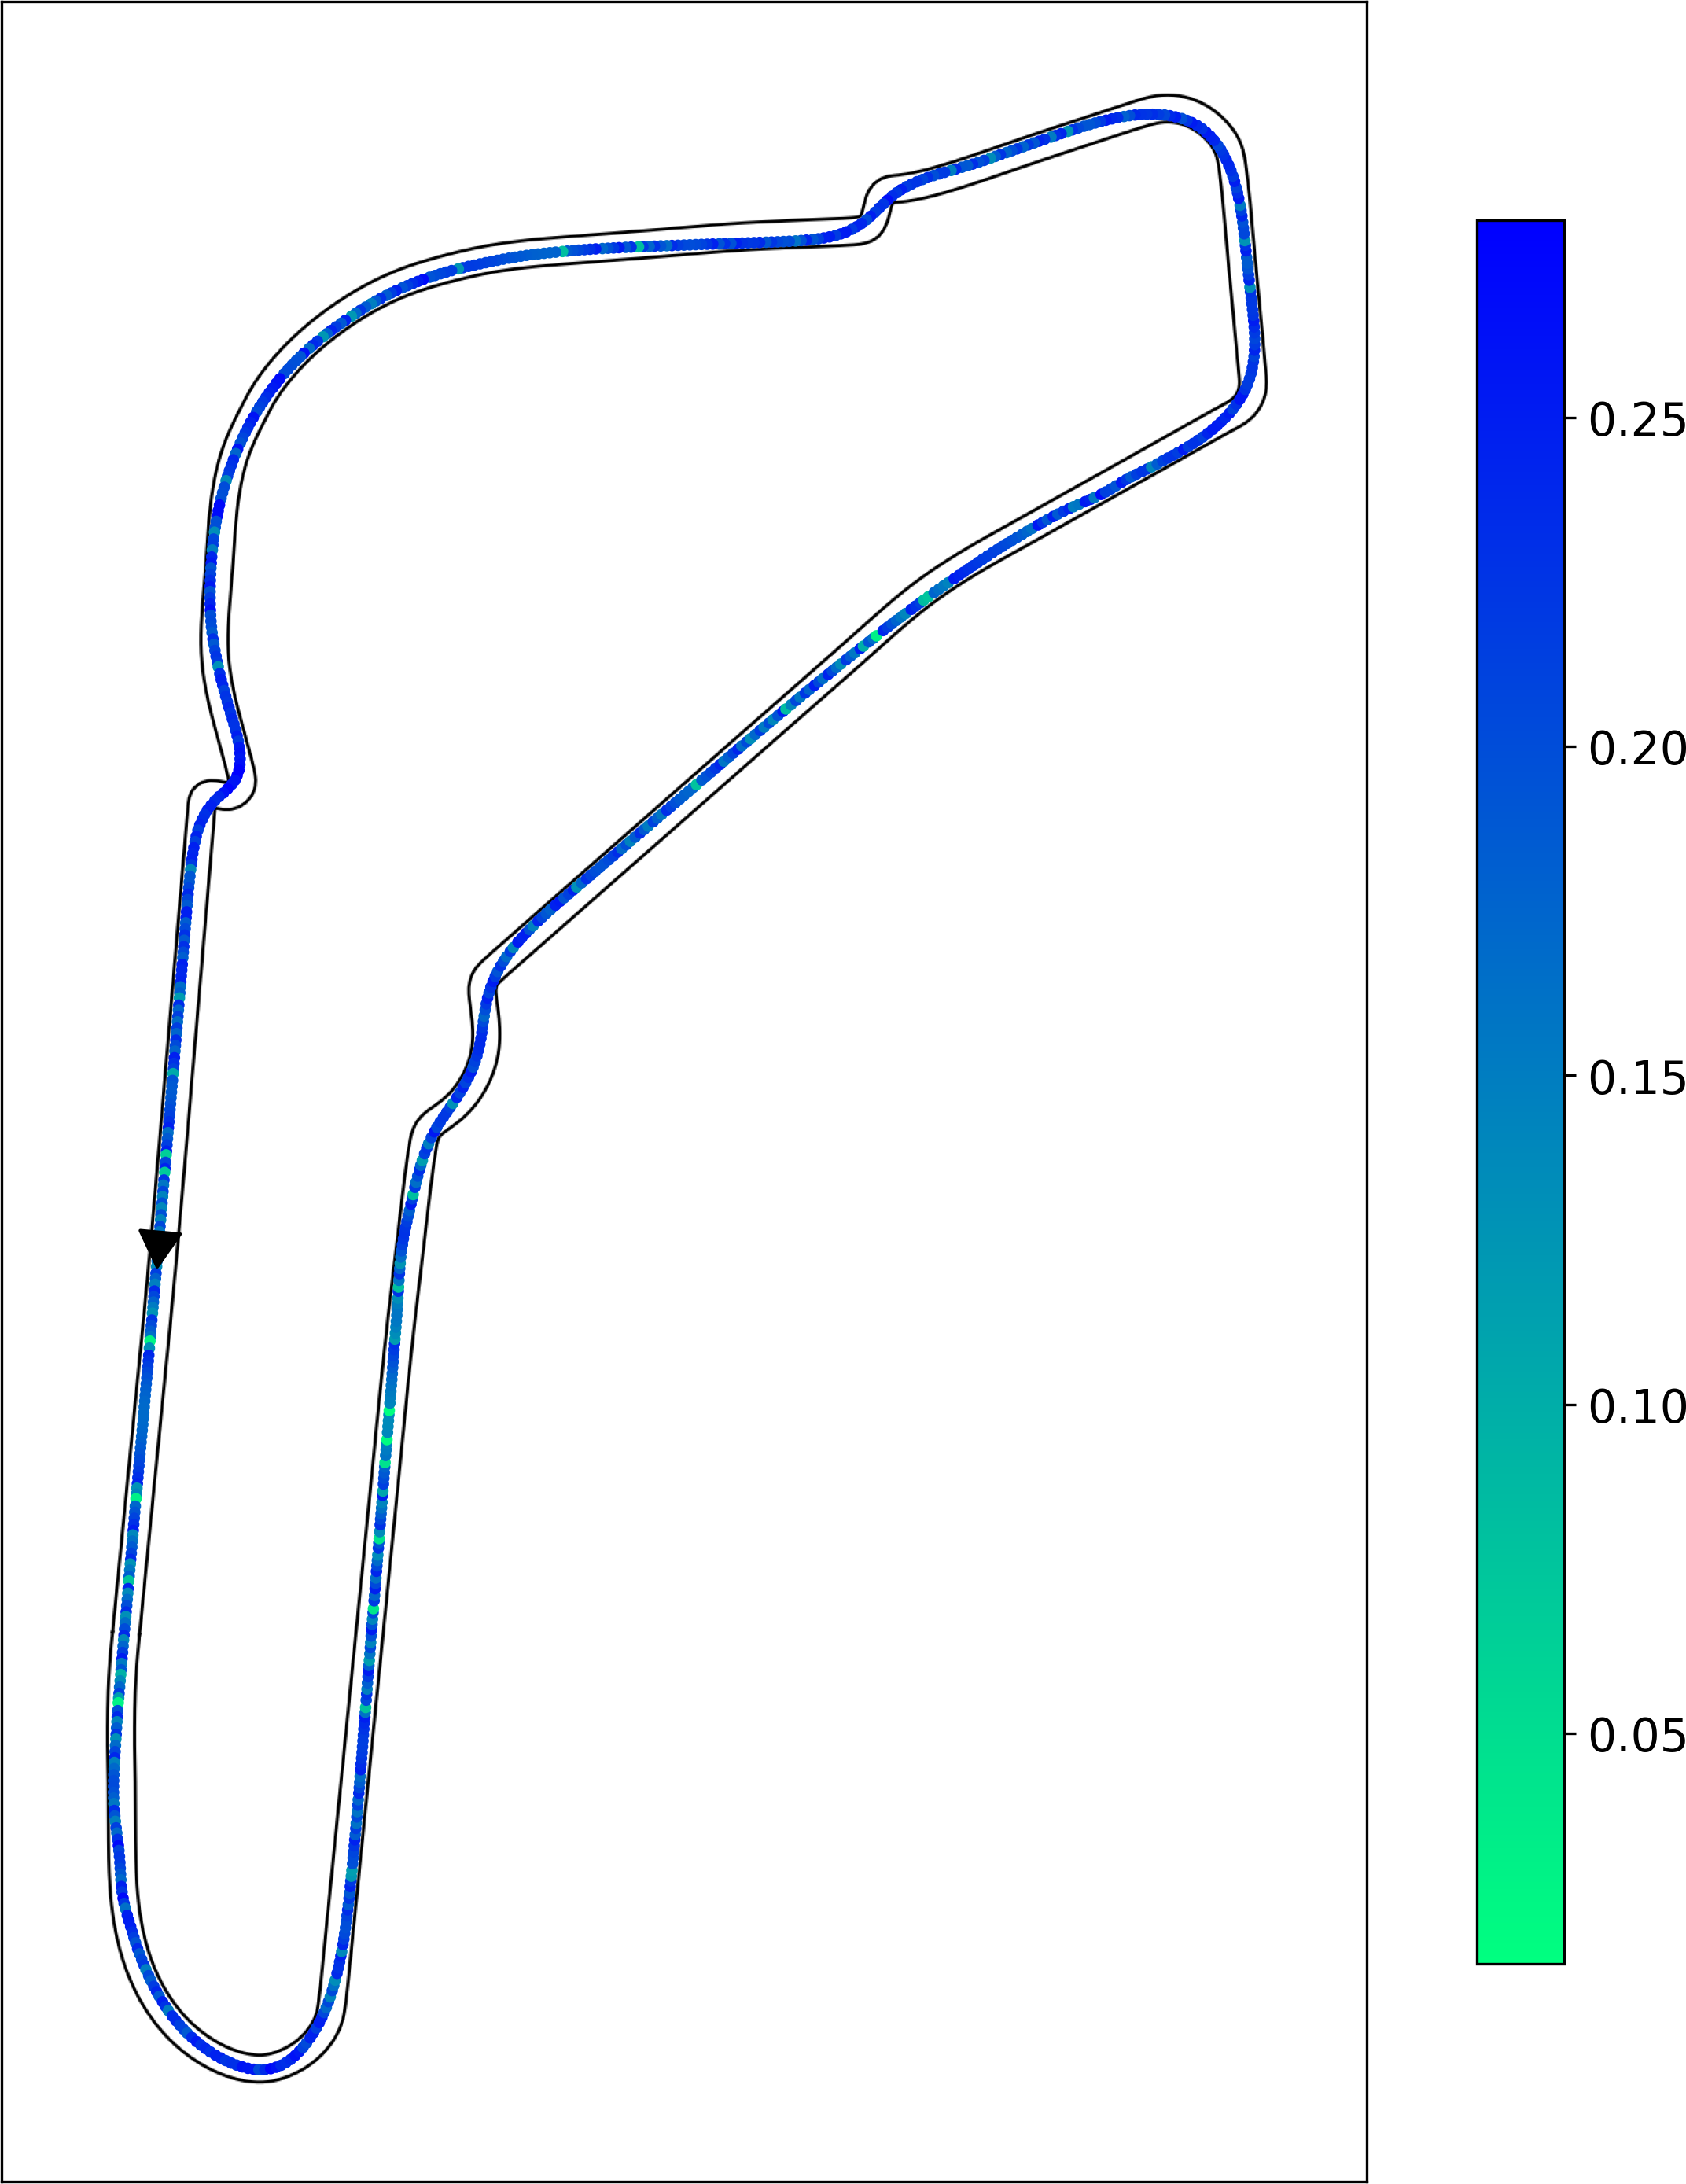
\includegraphics[width=0.75\textwidth]{images/monza_pp_crosstrack.png}
        \caption{\textit{Monza}}
        \label{fig:tracking_pp_monza}
    \end{subfigure}
    \caption{Crosstrack Error per \textit{Pure Pursuit}, usato come baseline.}
    \label{fig:fig17} % etichetta utilizzata per riferisi all'immagine
\end{figure}
Infatti, nella Fig.~\ref{fig:fig18} si noti
come tutti i profili di \textit{MPC} abbiano un colore più chiaro per 
la quasi totalità del percorso; in particolare, il profilo 
\textit{High Performance} è quello coi valori inferiori, seguito da 
\textit{Safe} -- confermando di riflesso il valore basso registrato per 
l'\textit{RMSE} -- e da \textit{Fast}. Inoltre, soprattutto per \textit{High Performance}, 
si può notare dal grafico il colore più marcato nella parte della 
\textit{curva a gomito} -- già vista nella Fig.~\ref{fig:curva_spa} -- 
poiché la ``taglia'' prima di ogni altro profilo.

\begin{figure}[H]
    \centering
    \begin{subfigure}[b]{0.3\textwidth}
        \centering
        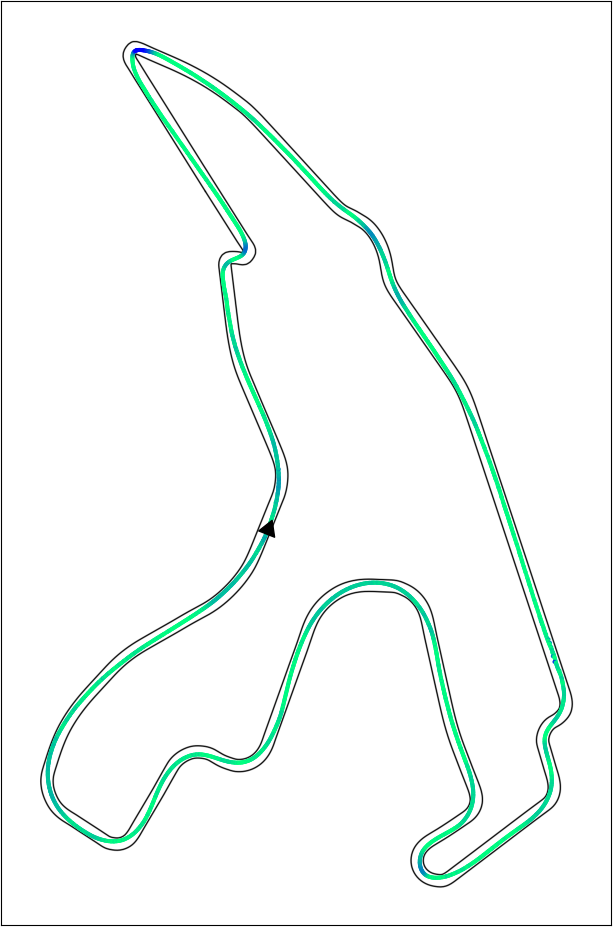
\includegraphics[width=\textwidth]{images/spa_mpc_hp_crosstrack.png} 
        \caption{\textit{High Performance}}
        \label{fig:tracking_hp_spa}
    \end{subfigure}
    %\hfill
    \begin{subfigure}[b]{0.3\textwidth}
        \centering
        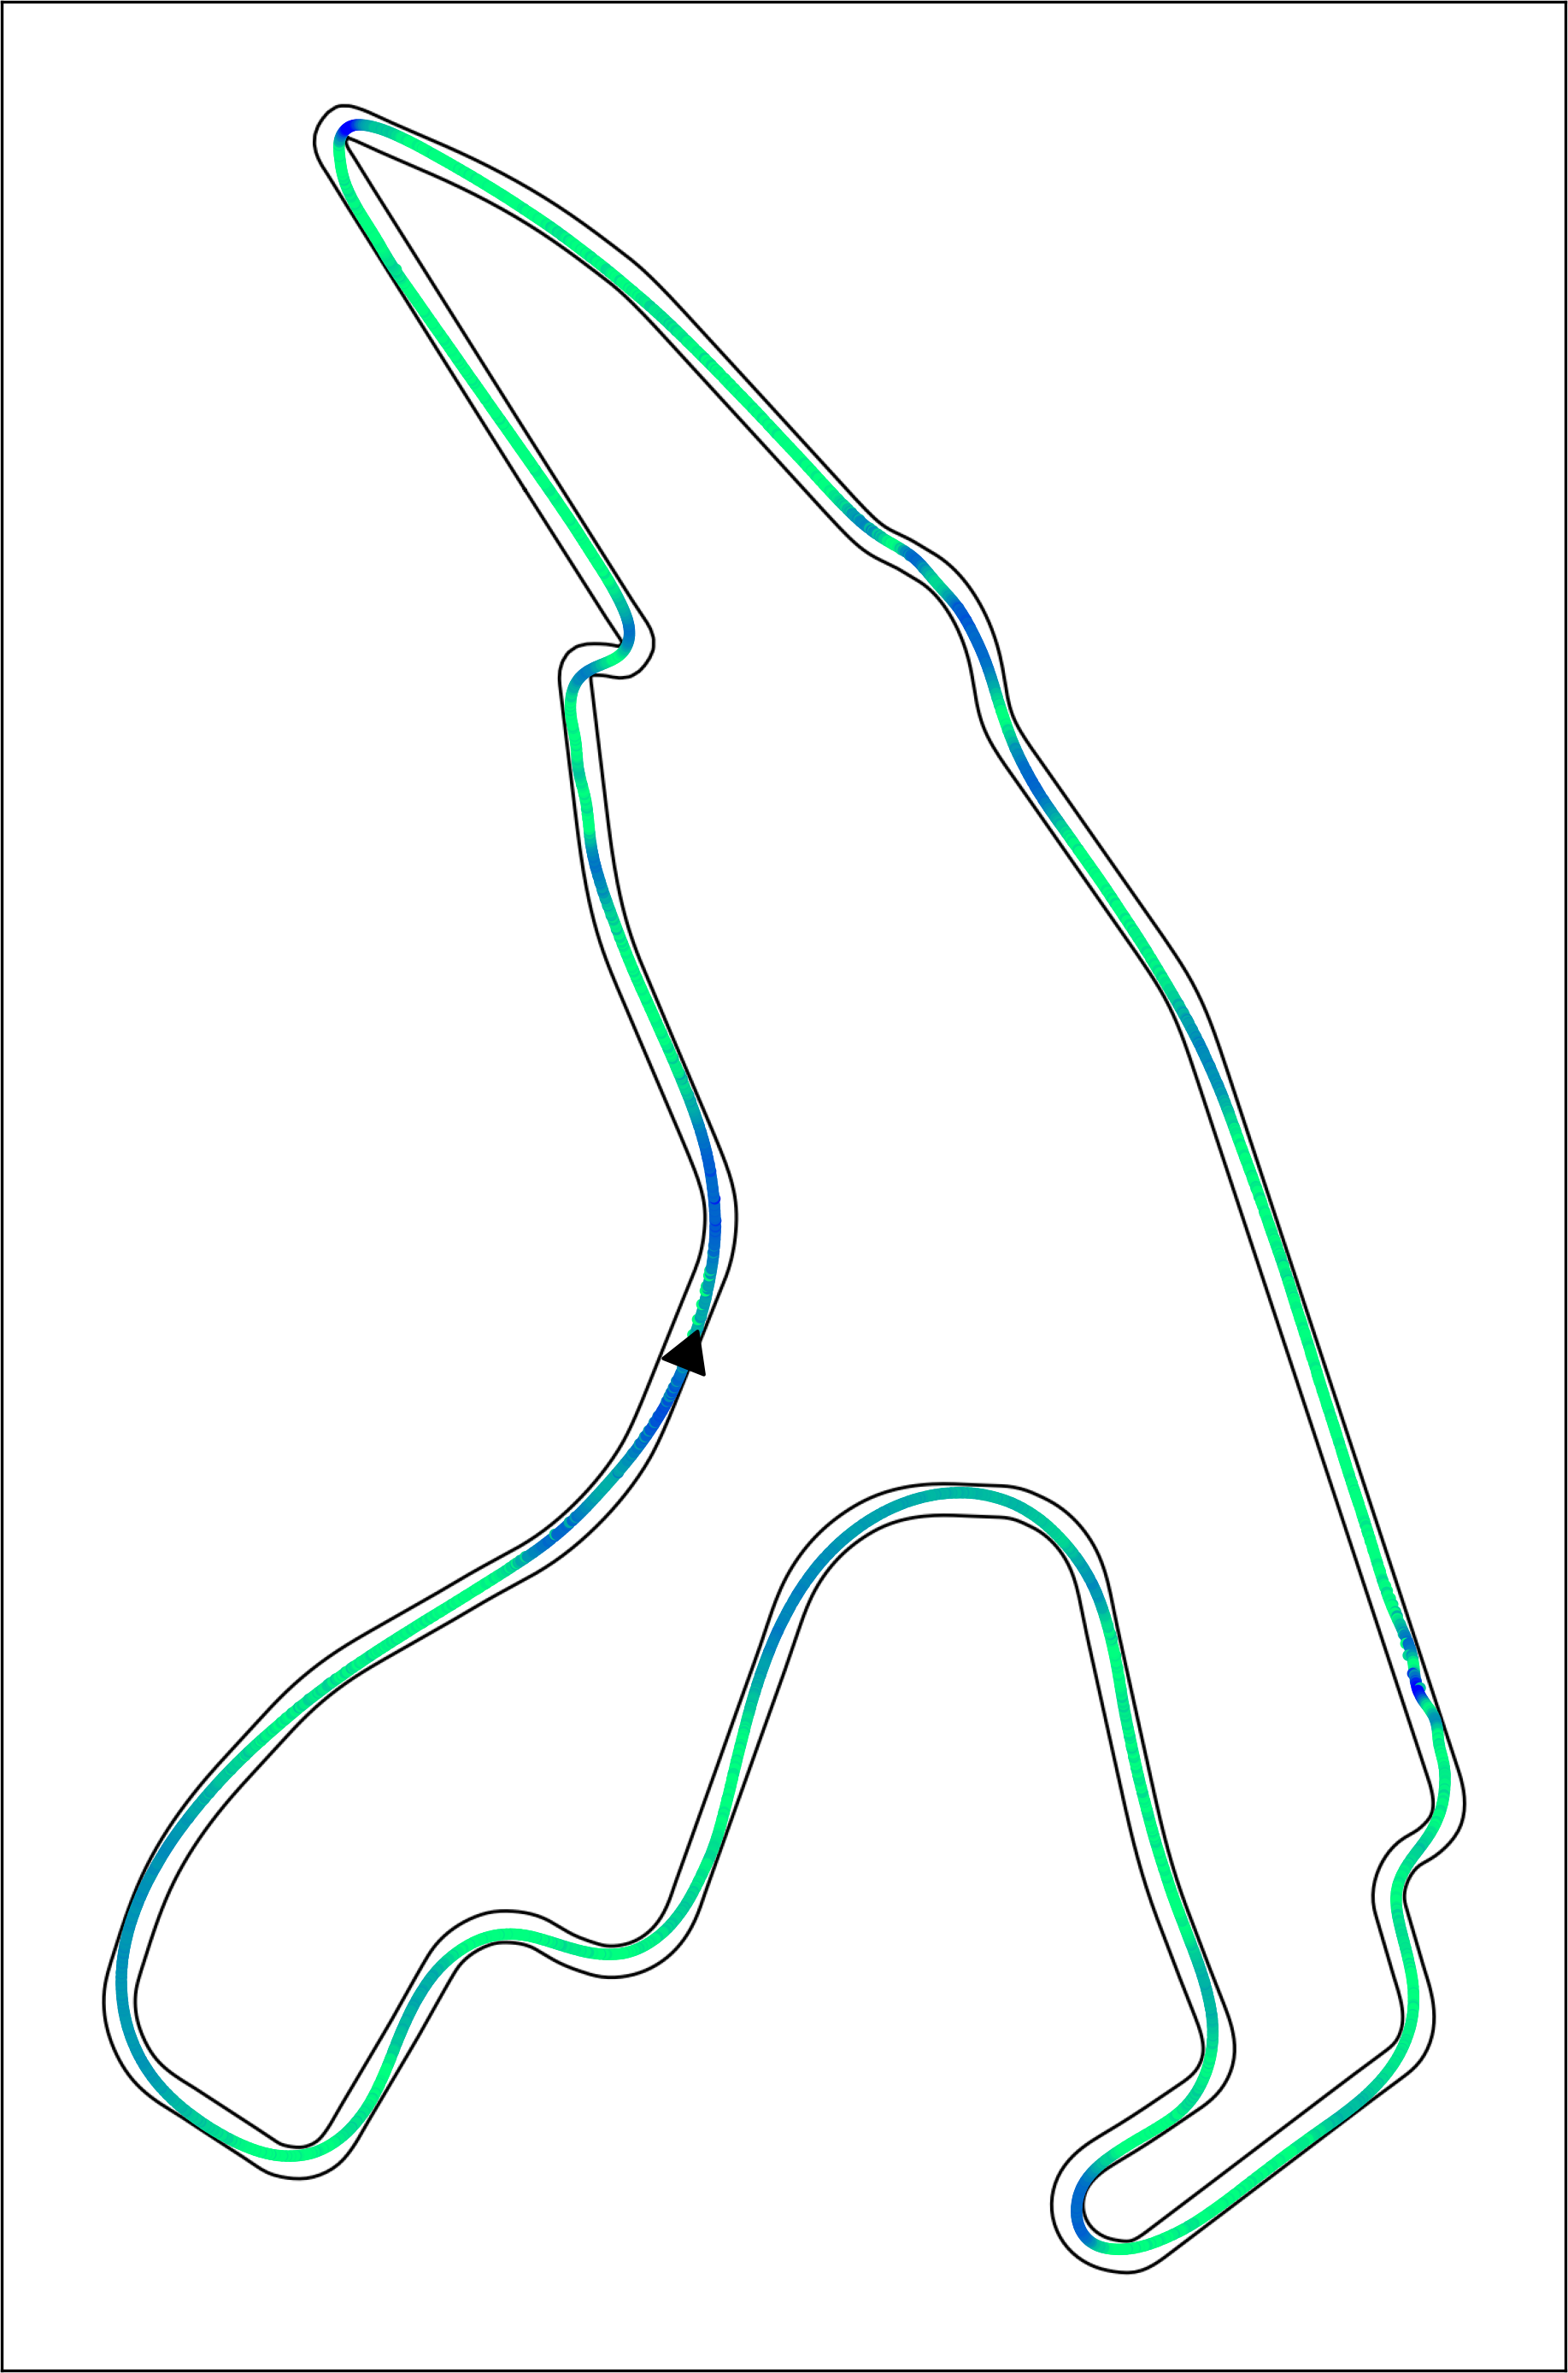
\includegraphics[width=\textwidth]{images/spa_mpc_fast_crosstrack.png}
        \caption{\textit{Fast}}
        \label{fig:tracking_fast_spa}
    \end{subfigure}
    %\hfill
    \begin{subfigure}[b]{0.366\textwidth}
        \centering
        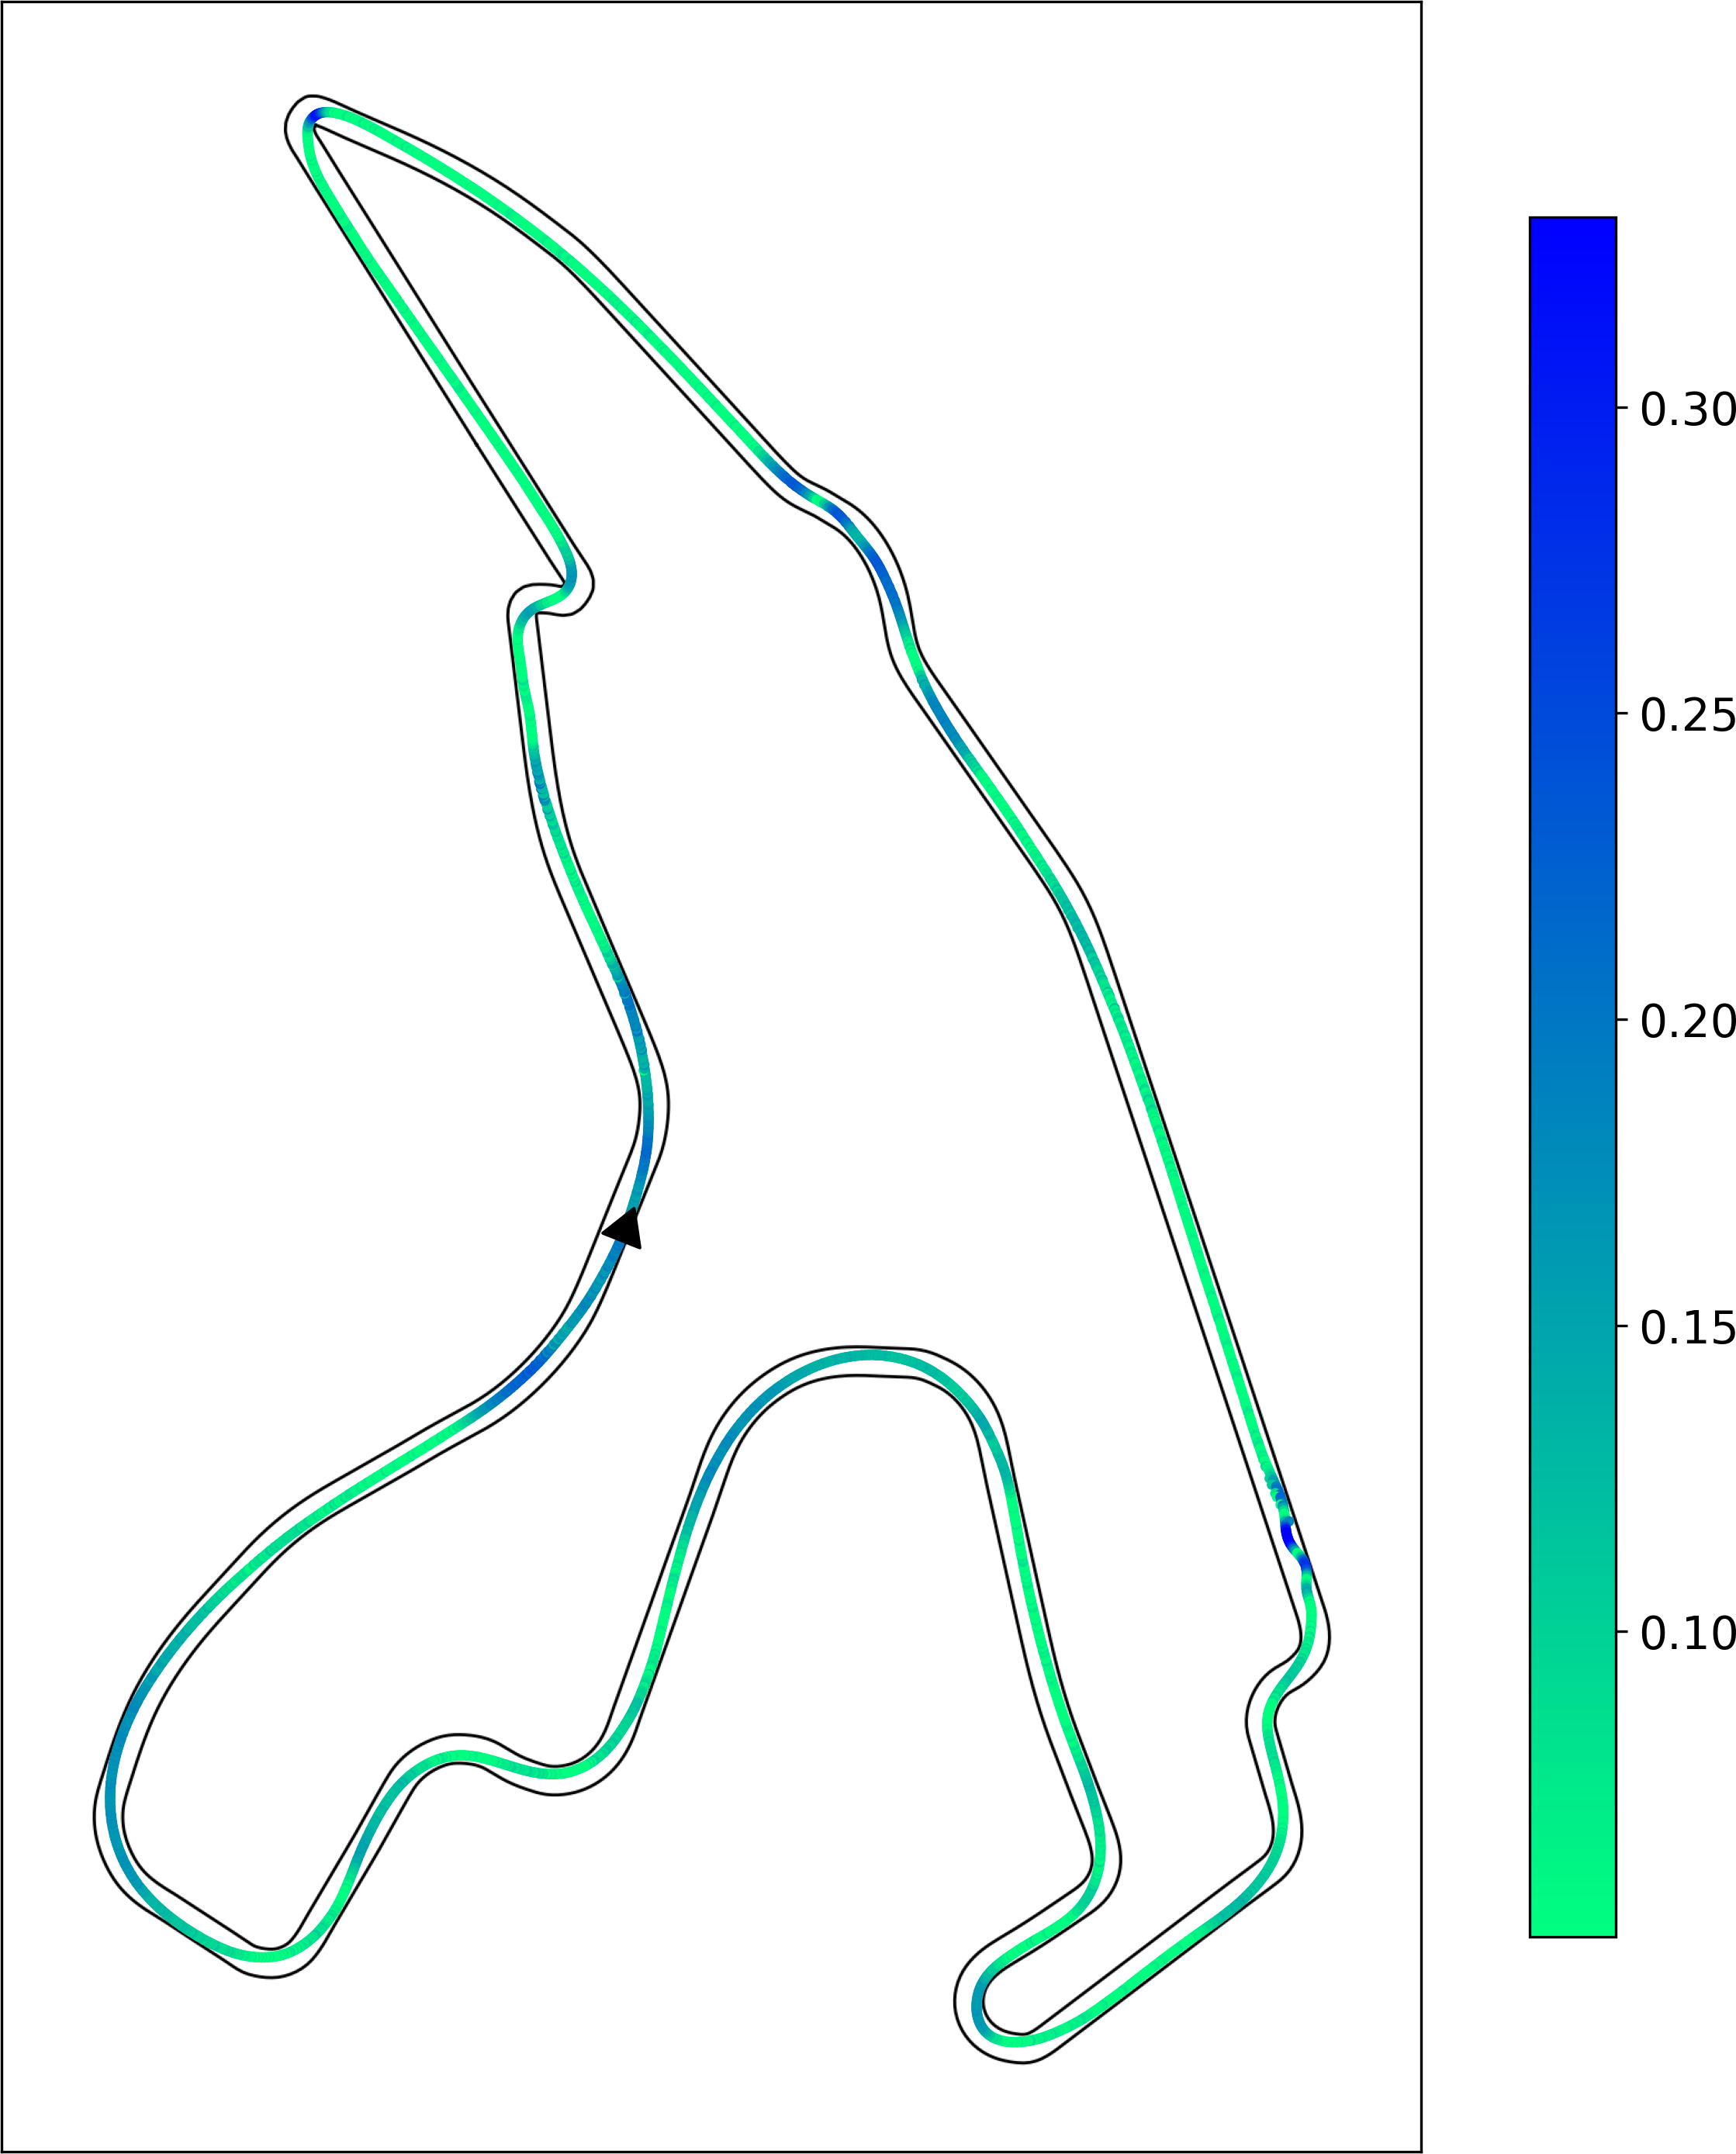
\includegraphics[width=\textwidth]{images/spa_mpc_safe_crosstrack.png}
        \caption{\textit{Safe}}
        \label{fig:tracking_safe_spa}
    \end{subfigure}
    \caption{Crosstrack Error per \textit{Spa}.}
    \label{fig:fig18} % etichetta utilizzata per riferisi all'immagine
\end{figure}
\begin{figure}[H]
    \centering
    \begin{subfigure}[b]{0.3\textwidth}
        \centering
        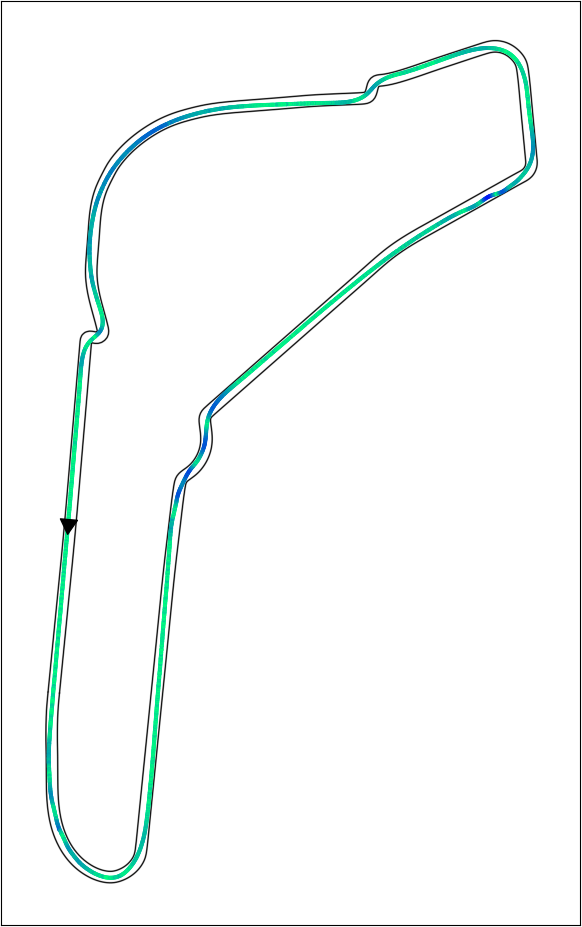
\includegraphics[width=\textwidth]{images/monza_mpc_hp_crosstrack.png} 
        \caption{\textit{High Performance}}
        \label{fig:tracking_hp_monza}
    \end{subfigure}
    \hfill
    \begin{subfigure}[b]{0.3\textwidth}
        \centering
        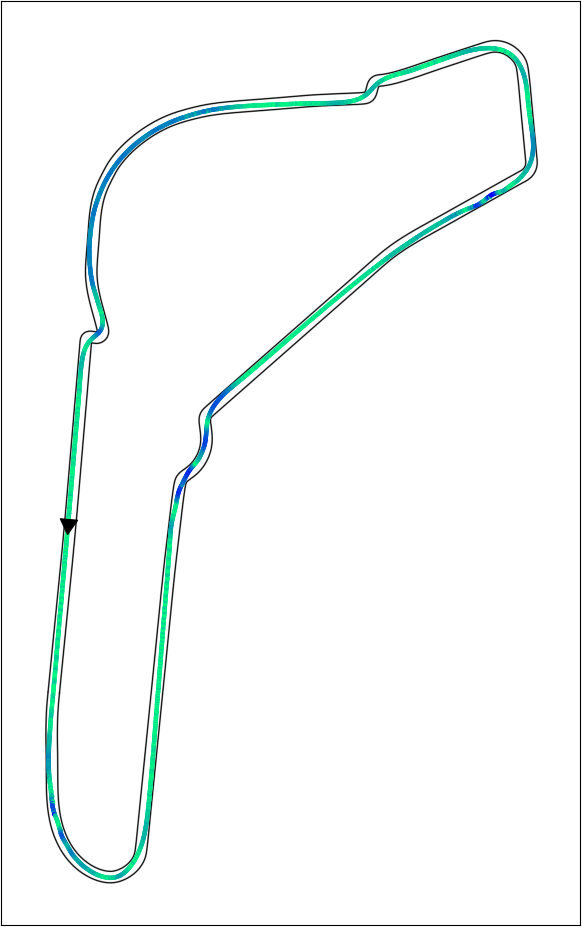
\includegraphics[width=\textwidth]{images/monza_mpc_fast_crosstrack.png}
        \caption{\textit{Fast}}
        \label{fig:tracking_fast_monza}
    \end{subfigure}
    \hfill
    \begin{subfigure}[b]{0.369\textwidth}
        \centering
        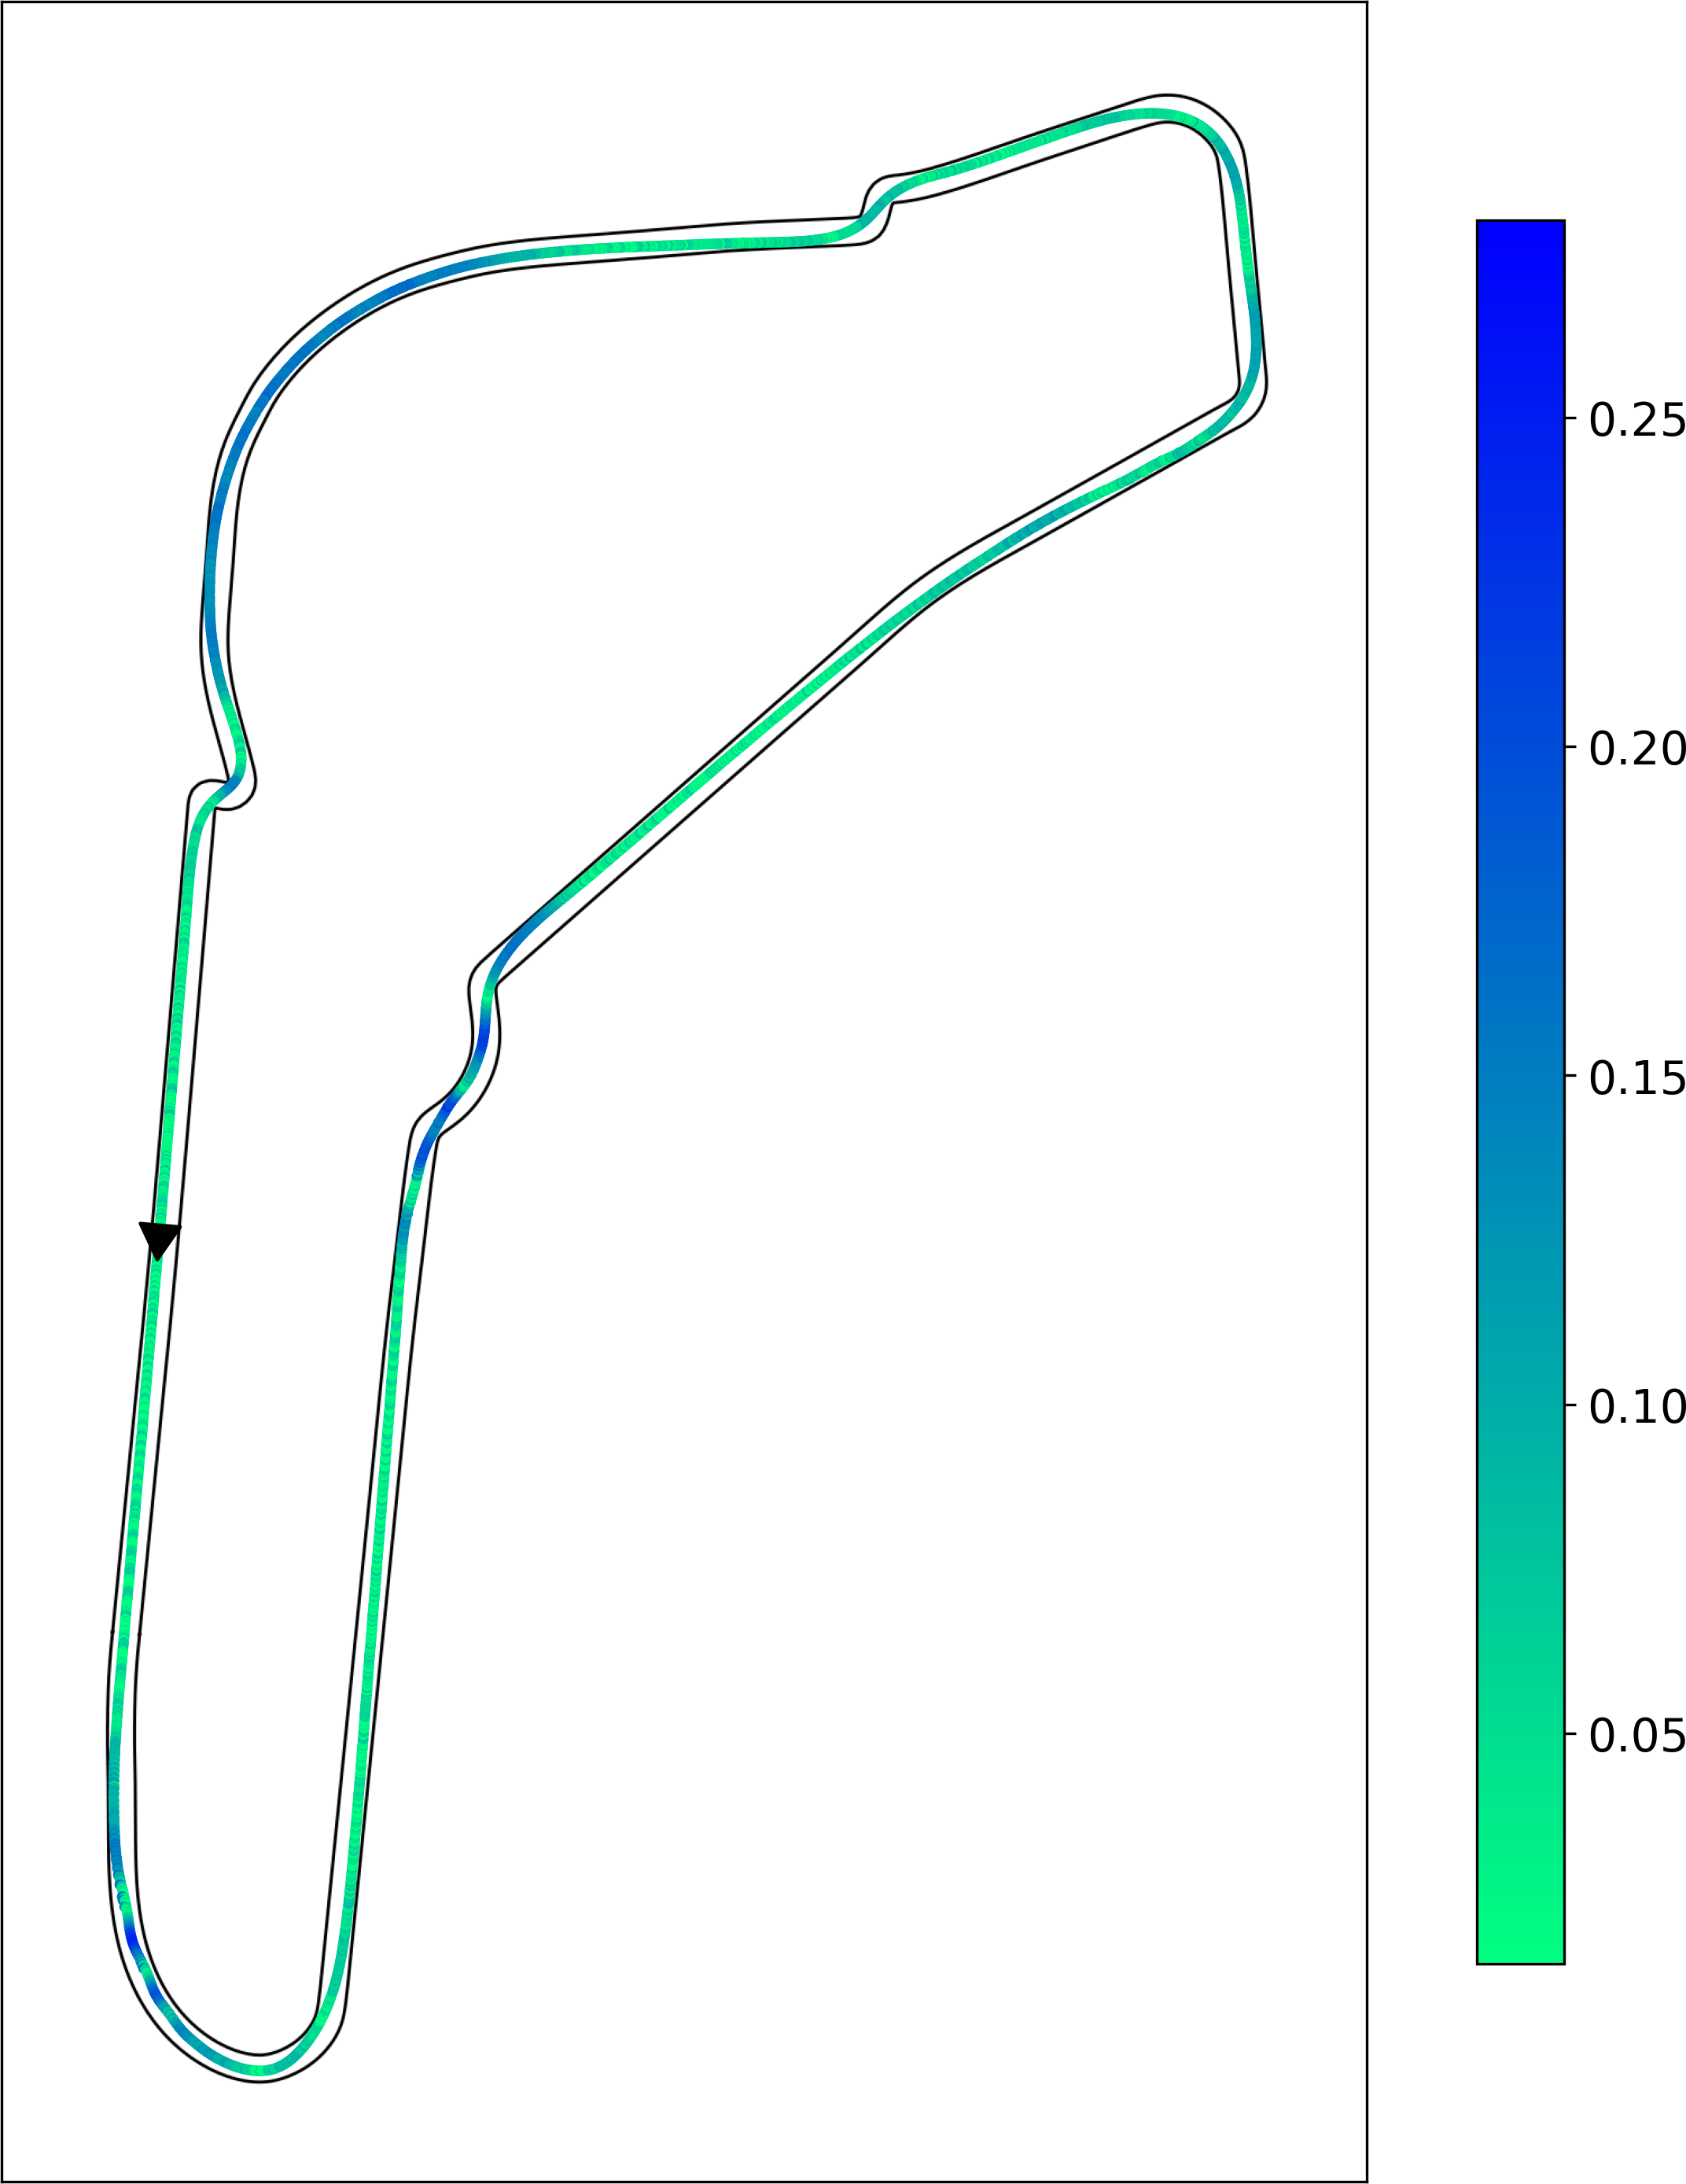
\includegraphics[width=\textwidth]{images/monza_mpc_safe_crosstrack.png}
        \caption{\textit{Safe}}
        \label{fig:tracking_safe_monza}
    \end{subfigure}
    \caption{Crosstrack Error per Monza.}
    \label{fig:fig19} % etichetta utilizzata per riferisi all'immagine
\end{figure}
La situazione è pressoché identica anche per i grafici della pista di 
\textit{Monza}, visualizzati nella Fig.~\ref{fig:fig19}. Unendo i 
risultati riepilogati nella sezione~\ref{subs:metrics}, con questi più 
quelli delle traiettorie mostrate in precedenza, si ottiene un quadro completo
relativo alle discrepanze tra i valori reali e quelli ideali, 
specialmente per quanto riguarda la deviazione dalla linea di riferimento, che è ciò si vuole minimizzare con \textit{MPC}.

\subsection{Velocità e Angolo di sterzata}
Si mostrano di seguito i grafici relativi al confronto della \textit{velocità} e 
dell'\textit{angolo di sterzata} per ogni zona dei due circuiti. Si precisa che viene mostrato
un valore ogni 10 metri per migliorare la resa grafica, così da notare maggiormente le differenze.

\begin{figure}[H]
    \centering
    \begin{subfigure}{\textwidth}
        \centering
        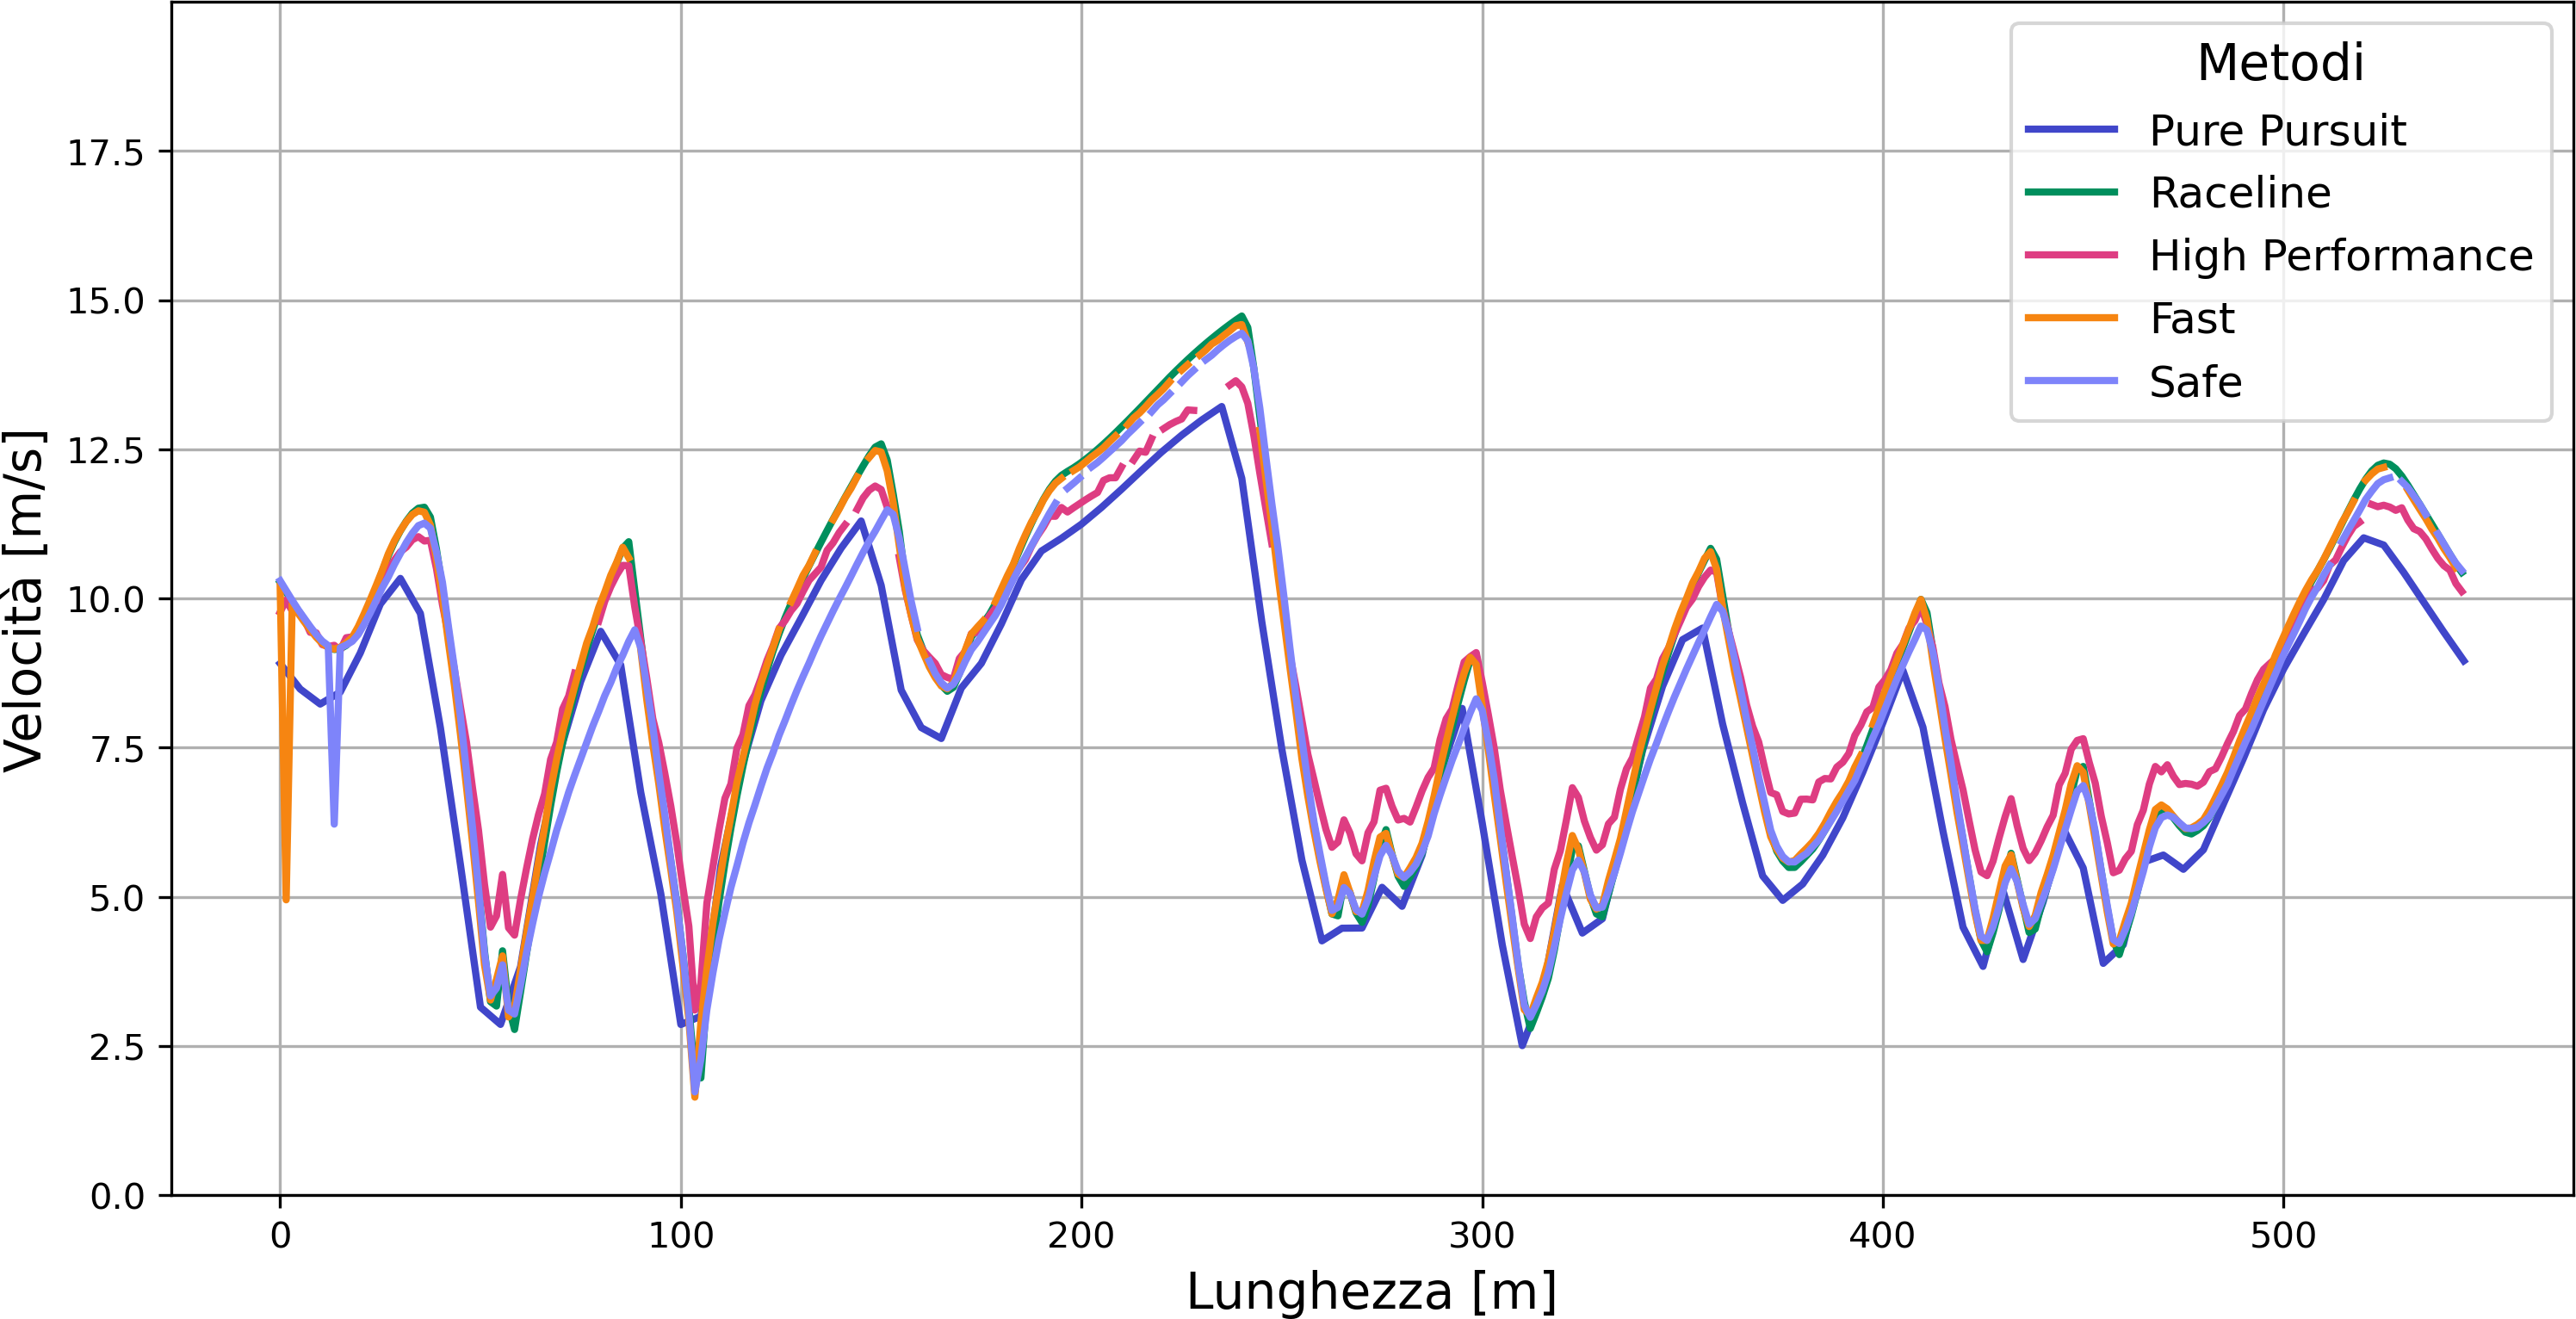
\includegraphics[scale=0.4]{images/spa_mpc_speed_comparisons.png} 
        \caption{\textit{Spa}}
        \label{fig:speed_comp_spa}
    \end{subfigure}
    %\vfill
    \begin{subfigure}{\textwidth}
        \centering
        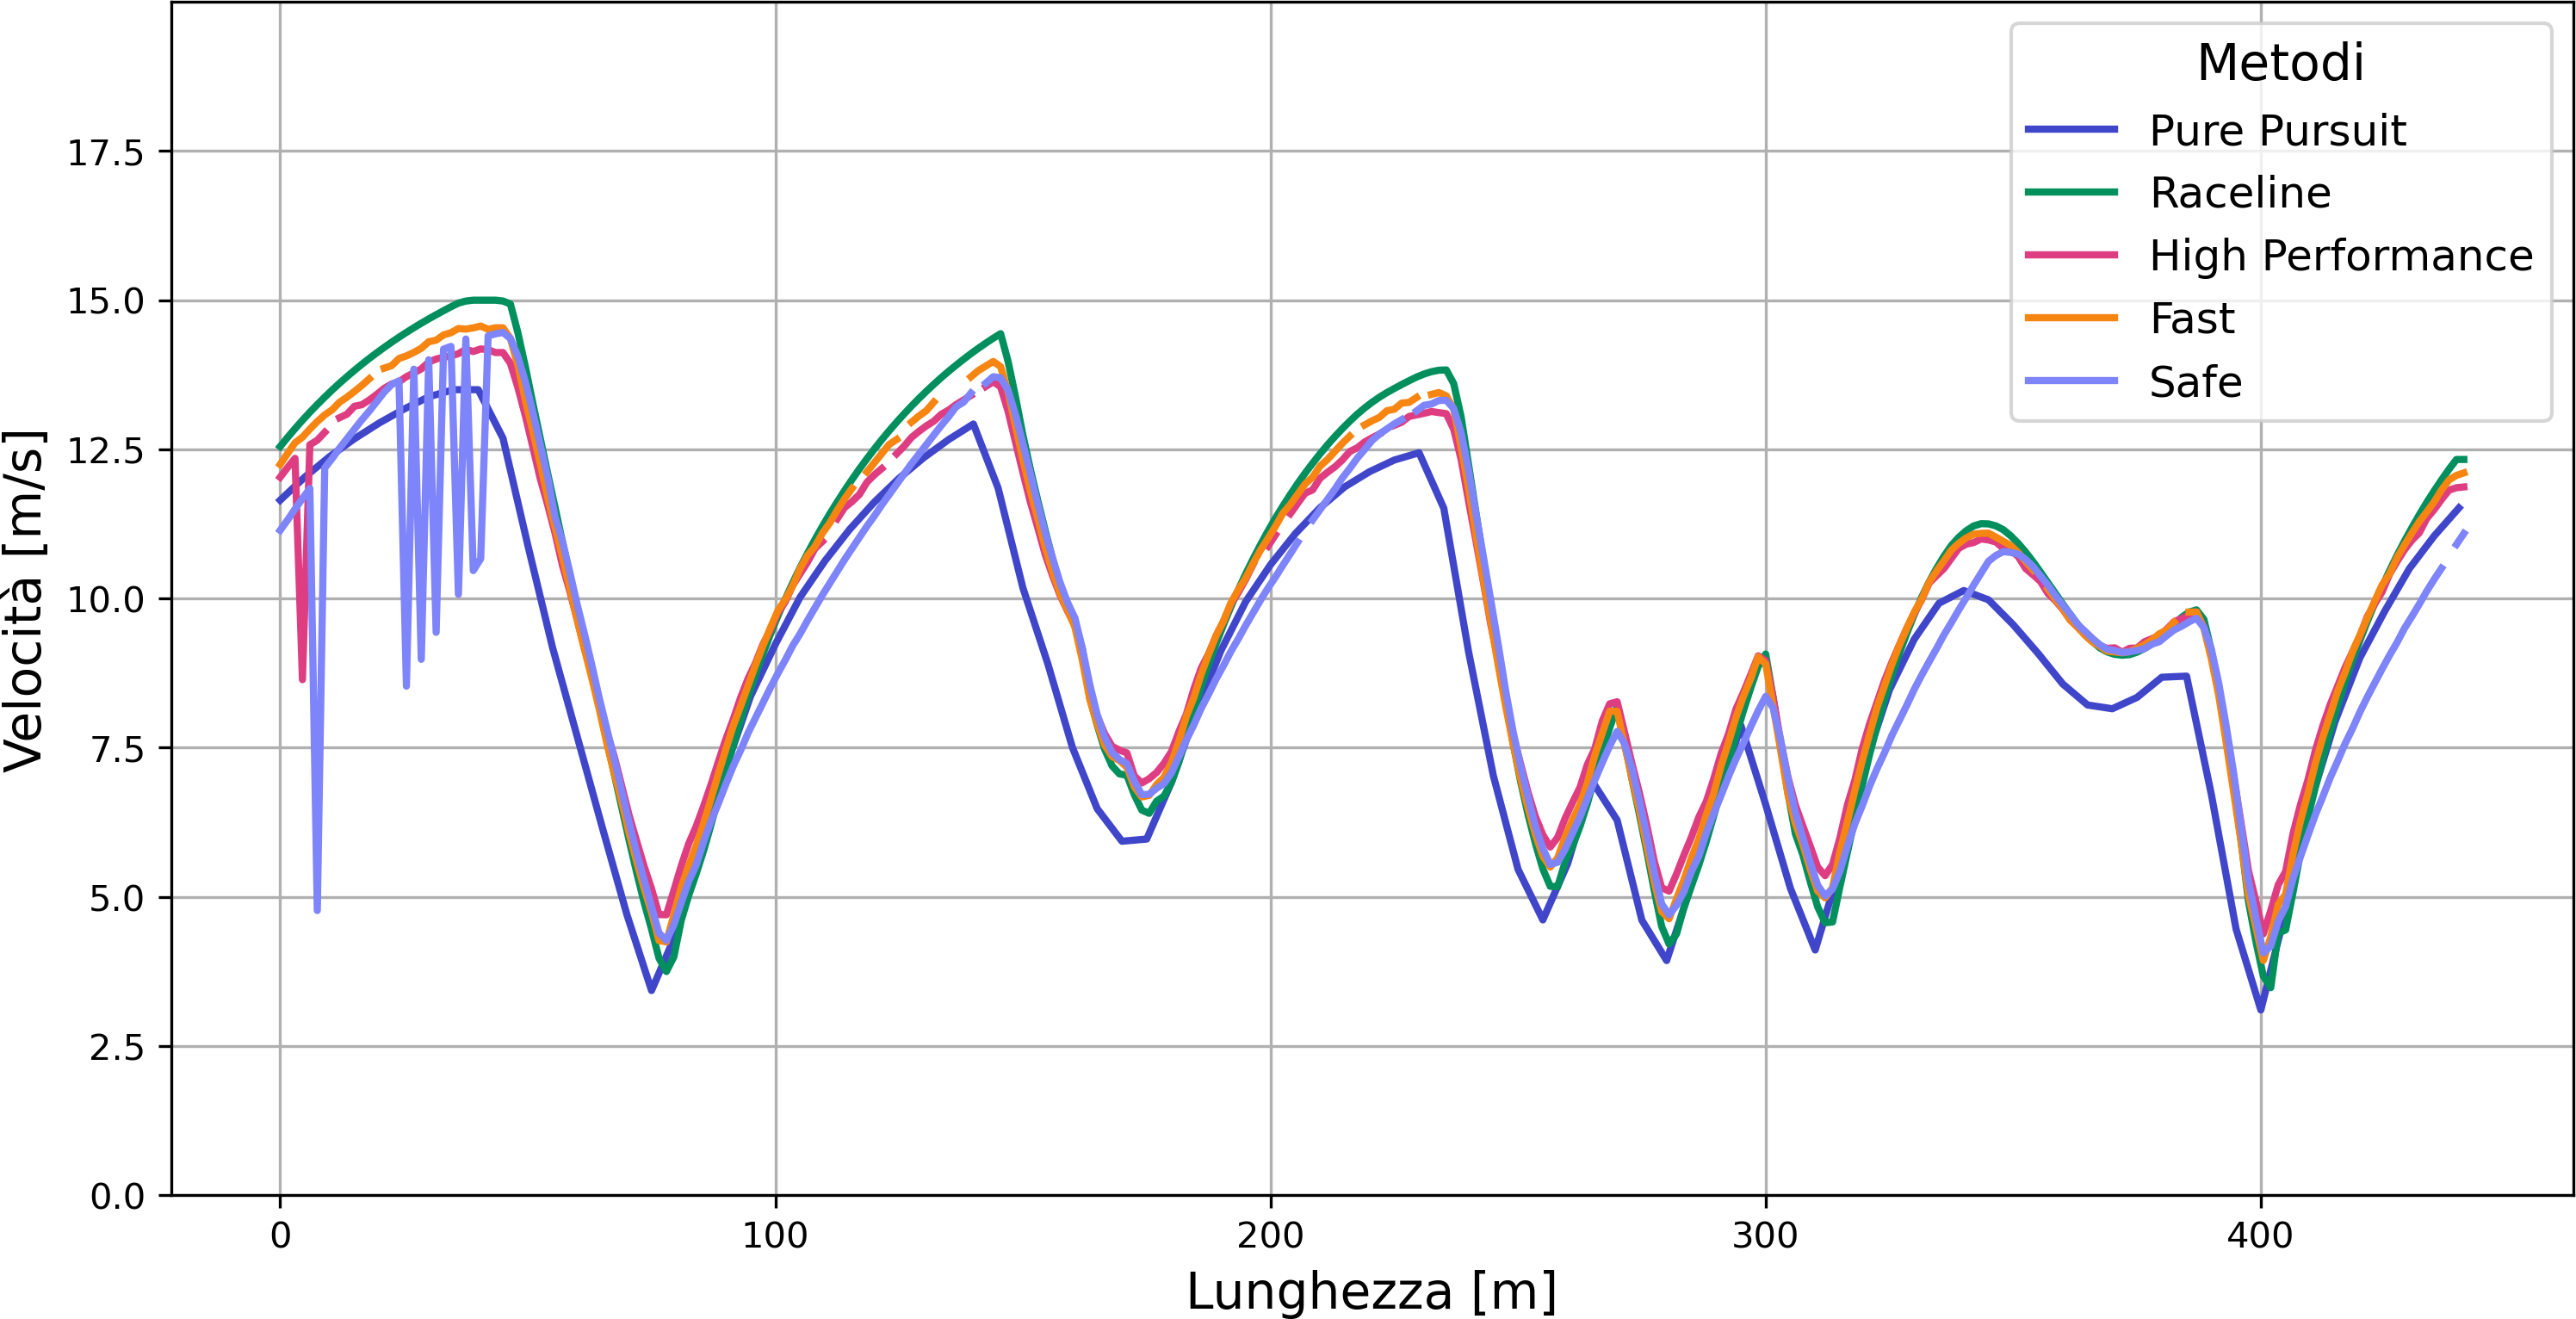
\includegraphics[scale=0.4]{images/monza_mpc_speed_comparisons.png}
        \caption{\textit{Monza}}
        \label{fig:speed_comp_monza}
    \end{subfigure}
    \caption{Confronto delle velocità su \textit{Spa} e \textit{Monza}.}
    \label{fig:fig20} % etichetta utilizzata per riferisi all'immagine
\end{figure}

Per quanto riguarda la velocità, si può osservare in Fig.~\ref{fig:fig20}
come i valori in \textit{Pure Pursuit} restino sempre inferiori agli
altri metodi: ciò accade poiché ha un profilo di velocità corrispondente al
90\% di quello indicato nel dataset della \textit{raceline}. Invece, per tutti
i profili di \textit{MPC}, nei primi 50 metri circa della pista di Monza,
si osserva una notevole variazione nella velocità applicata dall'algoritmo. 
Ciò è dovuto a un iniziale tempo di assestamento, in particolare per il profilo
\textit{Safe MPC} dato che parte più lentamente rispetto agli altri e con
un'accelerazione di 10 m/s$^2$.
Al contrario, gli altri profili mostrano un comportamento più attenuato, poiché
iniziano con velocità più elevate e un'accelerazione di 3 m/s$^2$.
Invece, si può osservare nella Fig.~\ref{fig:fig21} quanto appena descritto da un punto
di vista qualitativo, dove è stata riportata solo la parte iniziale del giro di 
\textit{Monza}. Si precisa che la scala cromatica è basata sui valori di velocità
della \textit{raceline} ottimale. In più, si osservino le variazioni cromatiche dei punti nello \textit{scatter plot}.

\begin{figure}[H]
    \centering
    \begin{subfigure}[b]{0.3\textwidth}
        \centering
        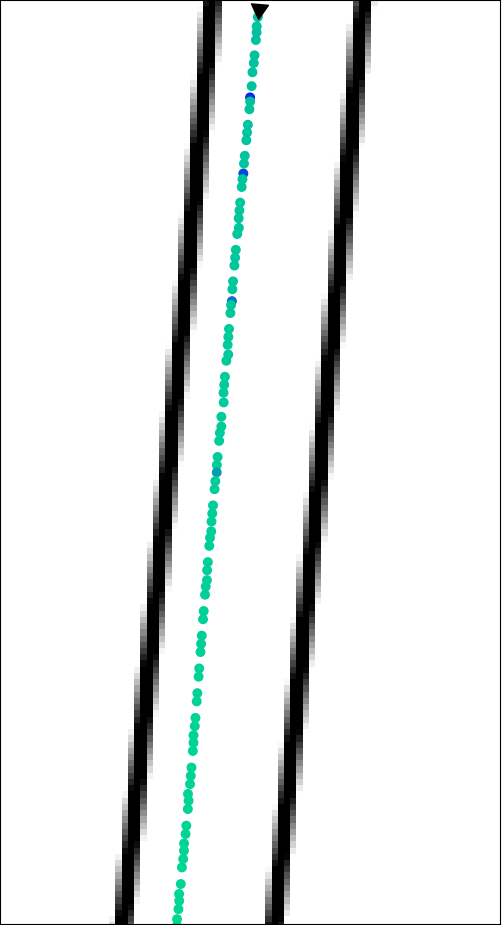
\includegraphics[width=\textwidth]{images/monza_zoom_mpc_high_performance_speed.png} 
        \caption{\textit{High Performance}}
        \label{fig:hp_speed}
    \end{subfigure}
    %\hfill
    \begin{subfigure}[b]{0.29\textwidth}
        \centering
        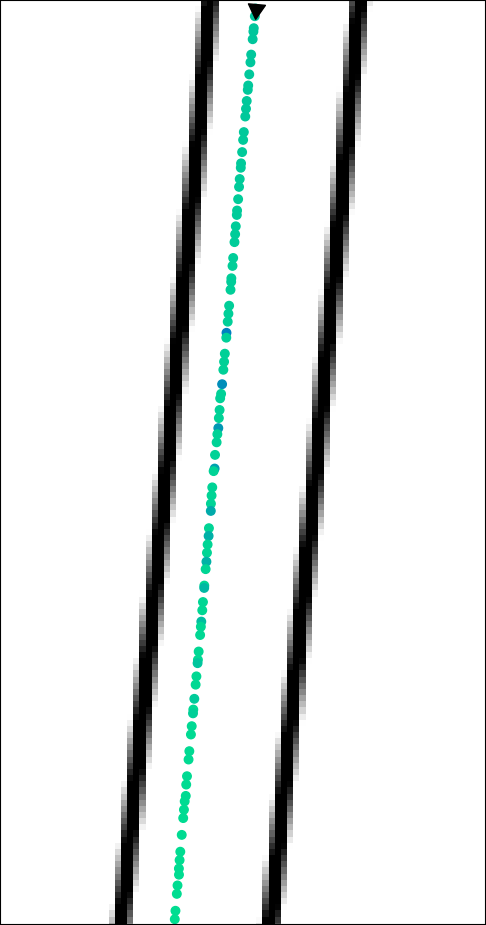
\includegraphics[width=\textwidth]{images/monza_zoom_mpc_fast_speed.png}
        \caption{\textit{Fast}}
        \label{fig:fast_speed}
    \end{subfigure}
    %\hfill
    \begin{subfigure}[b]{0.3805\textwidth}
        \centering
        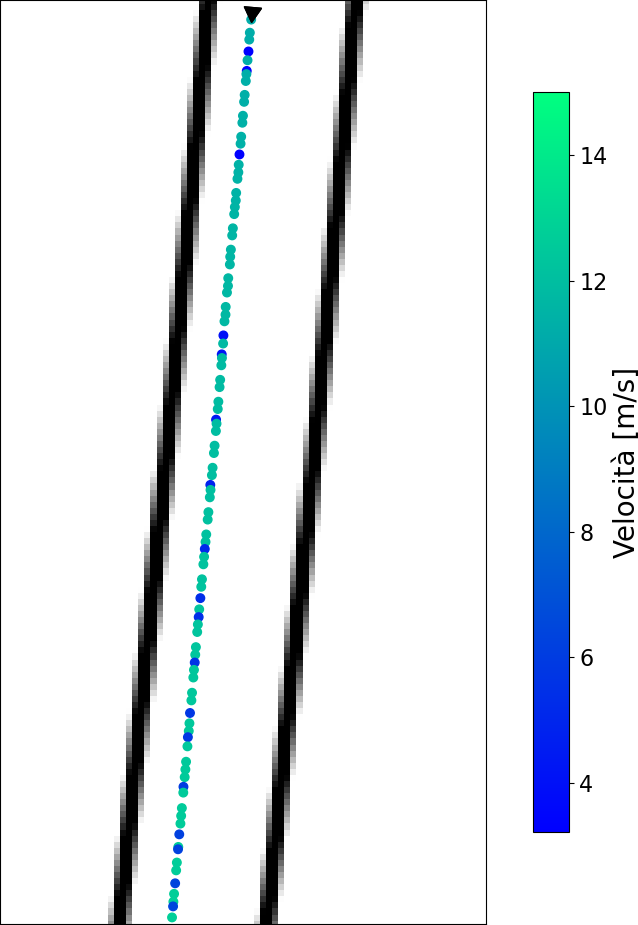
\includegraphics[width=\textwidth]{images/monza_zoom_mpc_safe_speed.png}
        \caption{\textit{Safe}}
        \label{fig:safe_speed}
    \end{subfigure}
    \caption{Confronto tra i metodi di \textit{MPC} su \textit{Monza}.}
    \label{fig:fig21} % etichetta utilizzata per riferisi all'immagine
\end{figure}

Dopo questa fase iniziale, per la pista di \textit{Monza} le velocità 
dei tre metodi sono molto simili a quella di riferimento data dalla 
\textit{raceline ottima}. Invece, per quella di \textit{Spa}, il profilo
\textit{High Performance} tende a superare la velocità di riferimento dalla seconda metà del tracciato.

Viene visualizzato graficamente anche l'angolo di sterzata $\delta$ attraverso il confronto dei
valori applicati dal \textit{Pure Pursuit} con quelli delle tre configurazioni di \textit{MPC}.

\begin{figure}[H]
    \centering
    \begin{subfigure}{\textwidth}
        \centering
        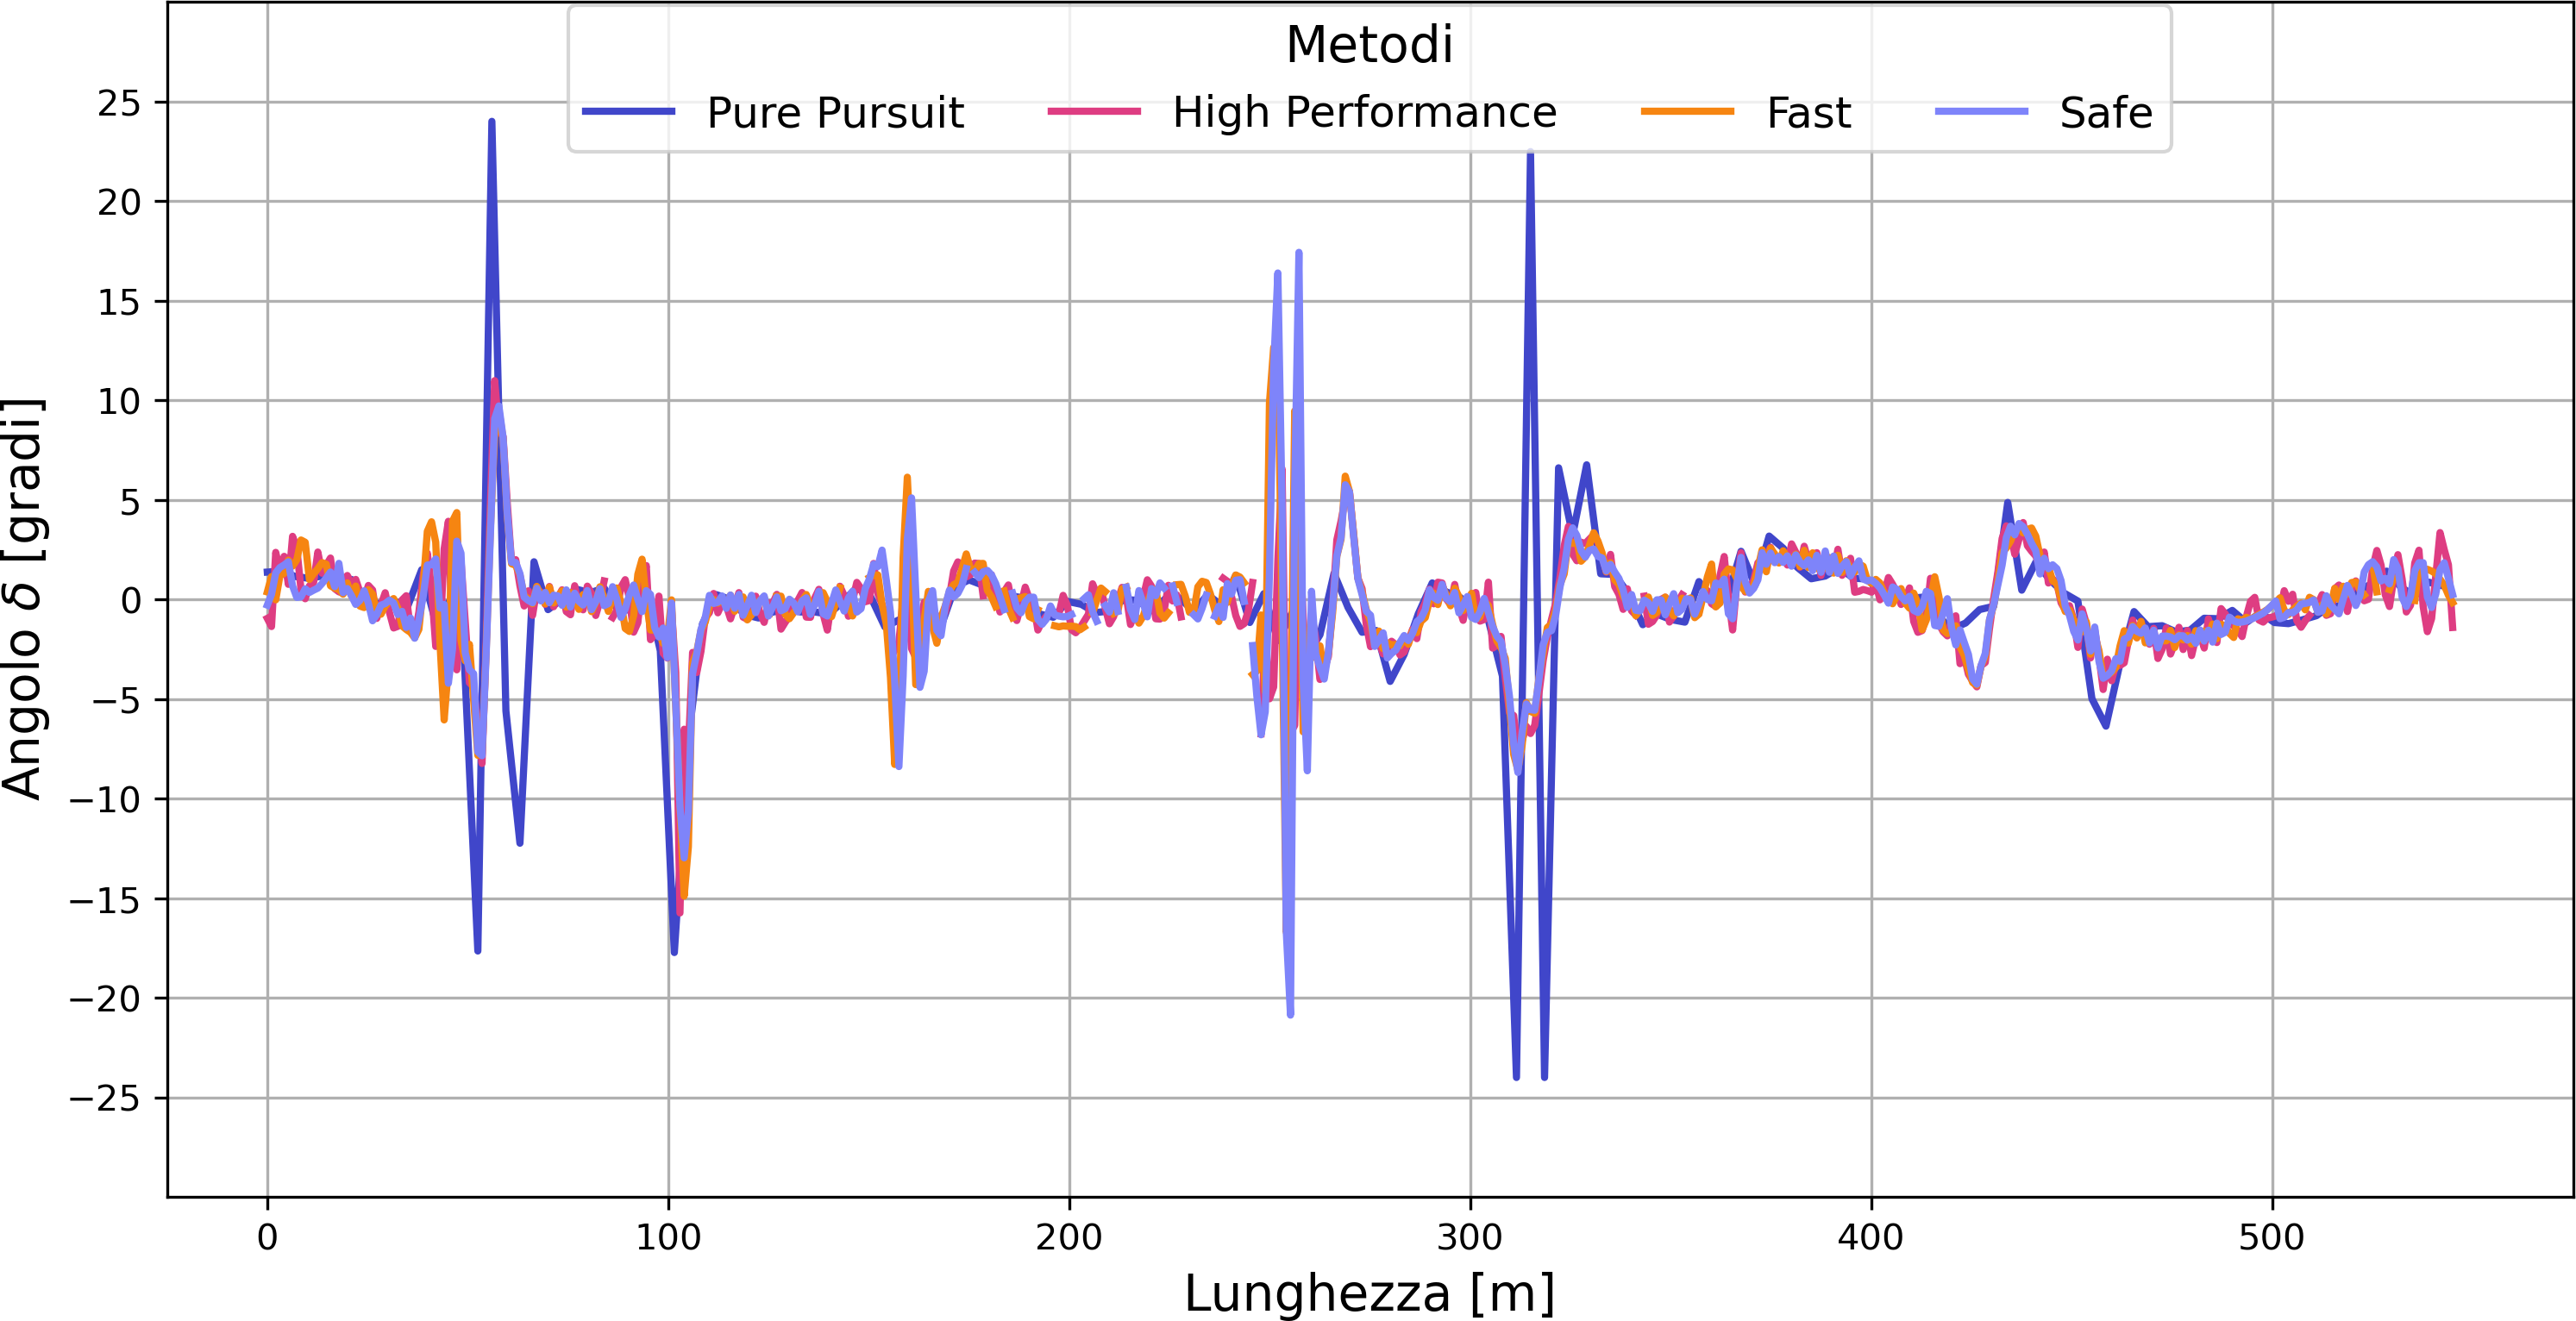
\includegraphics[scale=0.4]{images/spa_mpc_theta_comparisons.png} 
        \caption{\textit{Spa}}
        \label{fig:delta_comp_spa}
    \end{subfigure}
    %\vfill
    \begin{subfigure}{\textwidth}
        \centering
        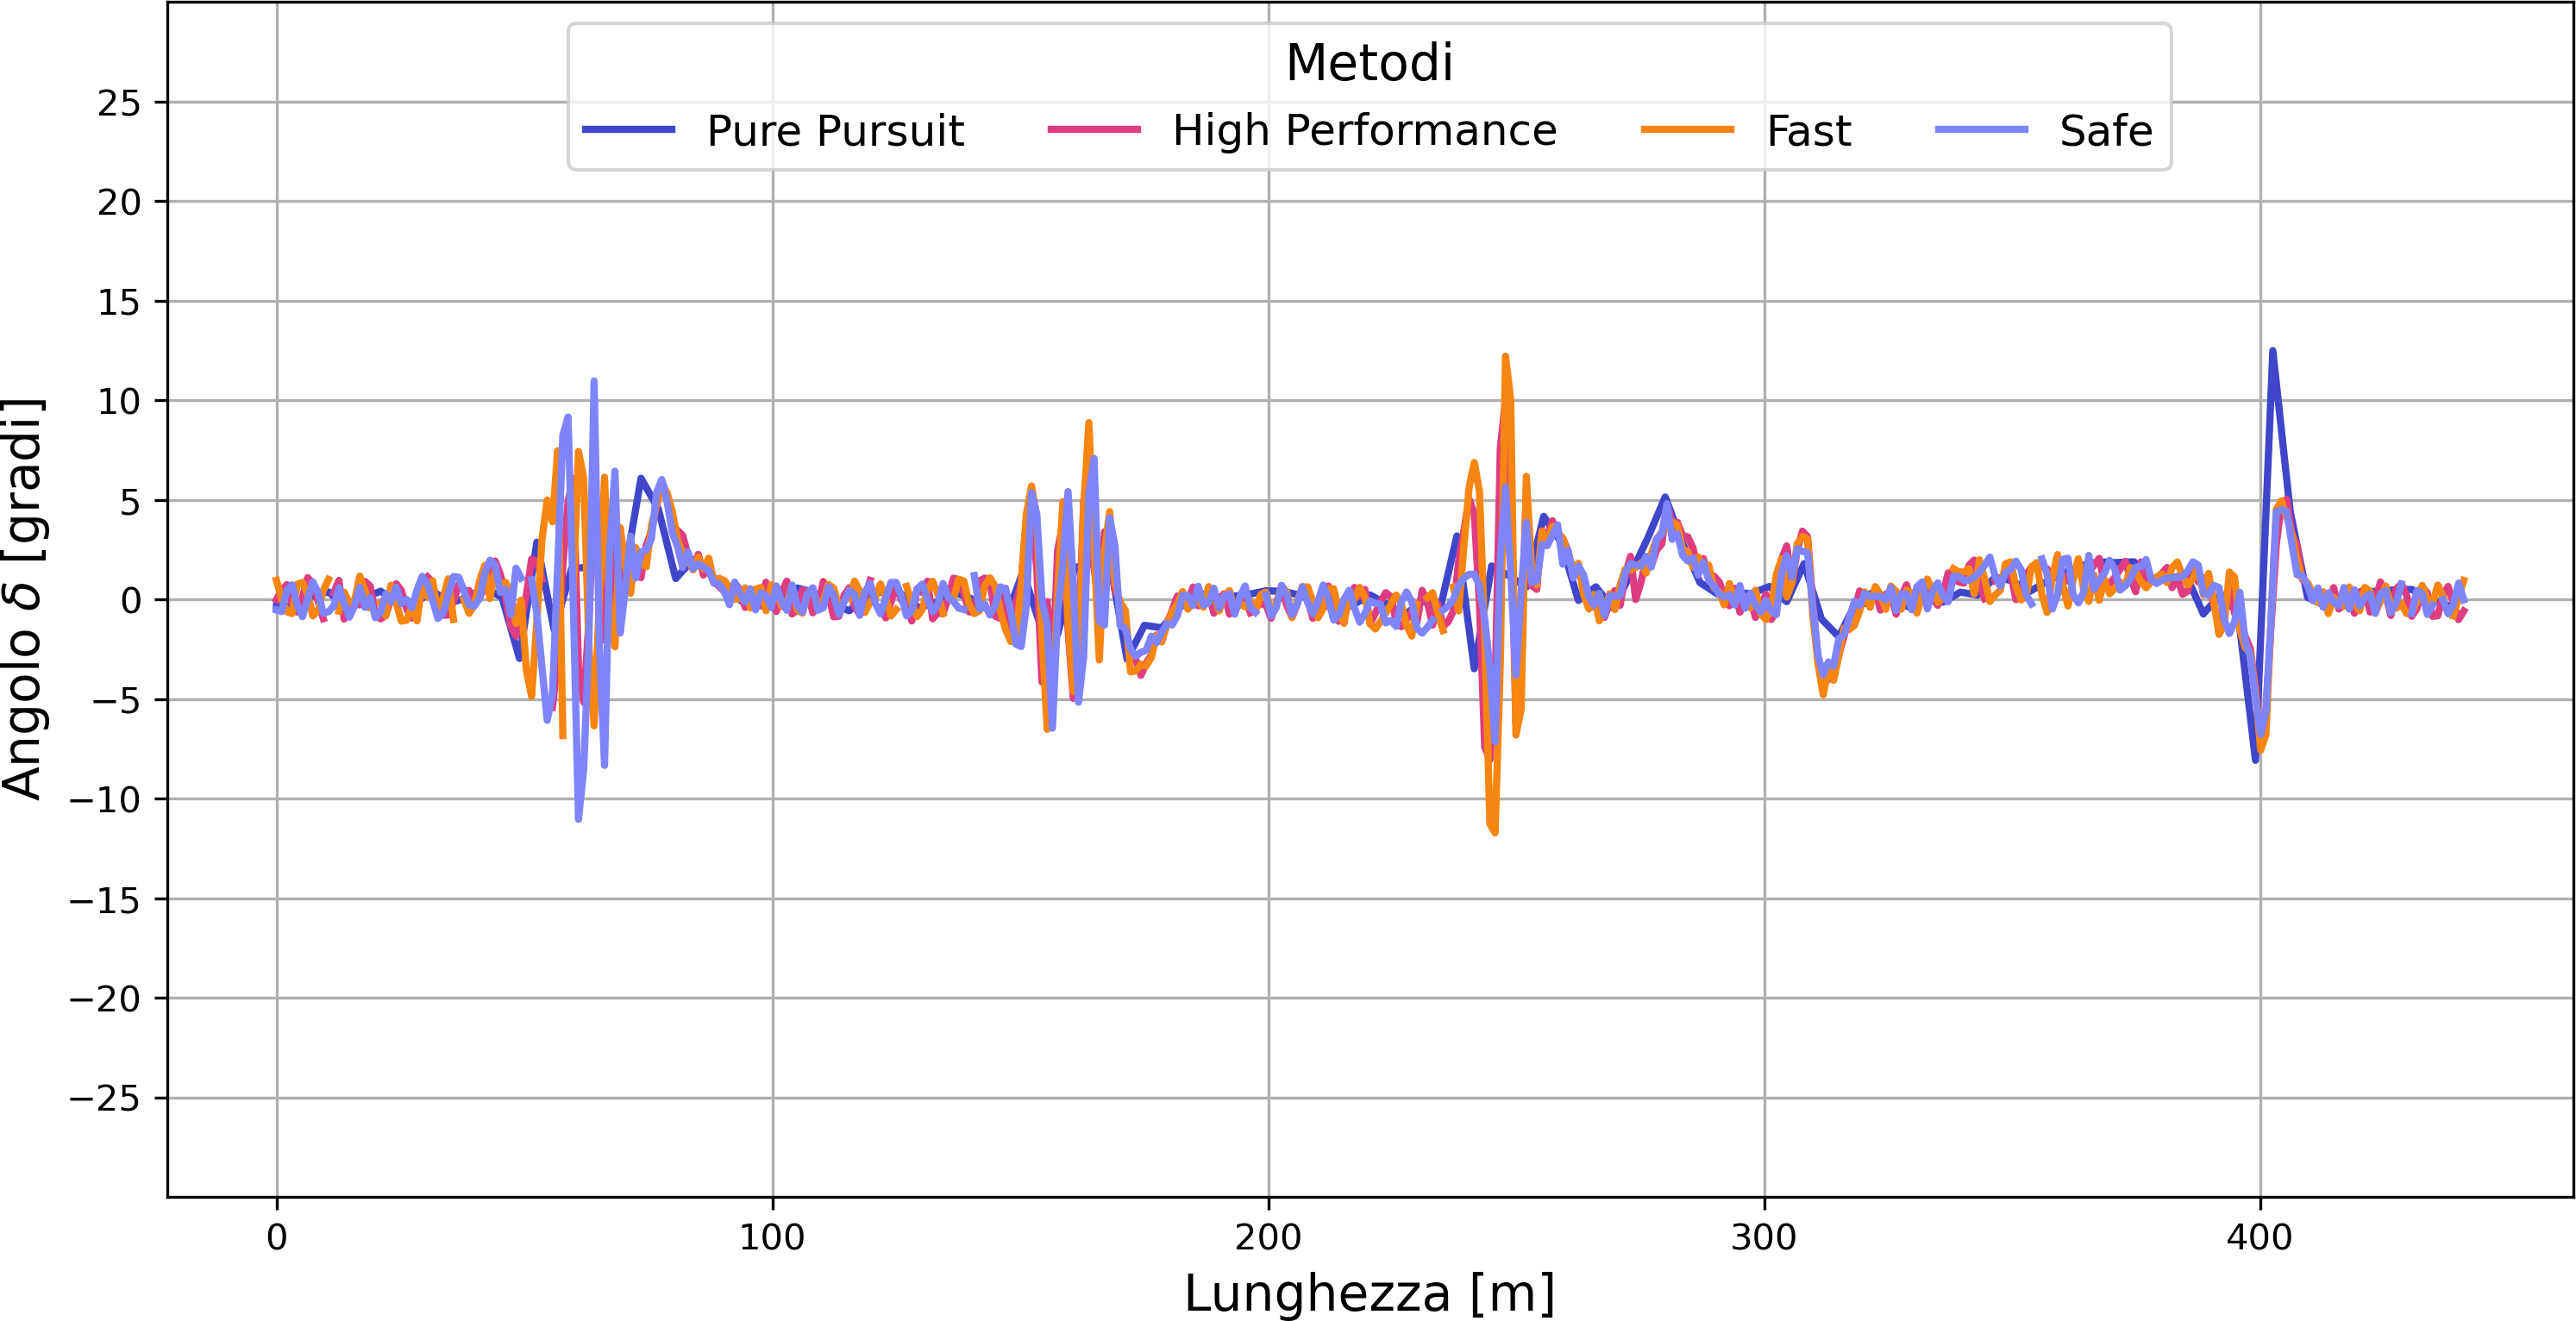
\includegraphics[scale=0.4]{images/monza_mpc_theta_comparisons.png}
        \caption{\textit{Monza}}
        \label{fig:delta_comp_monza}
    \end{subfigure}
    \caption{Confronto degli angoli di sterzata applicati su \textit{Spa} e \textit{Monza}.}
    \label{fig:fig22} % etichetta utilizzata per riferisi all'immagine
\end{figure}
Come mostrato in Fig.~\ref{fig:fig22}, il \textit{Pure Pursuit} presenta 
angoli di sterzata massimi più elevati in specifici punti di \textit{Spa} 
rispetto a Monza, mentre altrove è generalmente simile a \textit{MPC}.
Infatti, i profili \textit{MPC} mostrano angoli analoghi tra loro
su \textit{Spa}, con aumenti in certe zone per \textit{Safe} e 
\textit{Fast}, ma anche su \textit{Monza} si ha un comportamento simile. 
Dunque, in generale, i profili di \textit{MPC} hanno applicato angoli
assimilabili a quelli di \textit{Pure Pursuit}, a eccezione di certe zone di \textit{Spa}.
\chapter{Conclusioni}
In quest'ultimo capitolo si traggono le conclusioni sui risultati delle analisi svolte e
sui possibili sviluppi futuri di questo lavoro.

\label{chap:chap6}
\section{Risultati ottenuti}
Si è arrivati a realizzare un sistema di controllo avanzato che permette di 
ottimizzare l'attività del \textit{path tracking} attraverso l'implementazione
in \textit{Python} dell'algoritmo \textit{Model Predictive Control}.
Si è dunque in grado di seguire la linea di riferimento, ovvero la raceline generata dal \textit{planner}, con una 
traiettoria ottimale calcolata in tempo reale lungo l'intero percorso. Ciò permette di 
minimizzare la deviazione dalla linea di riferimento, che è stata misurata mediante il 
\textit{Crosstrack Error} e, inoltre, nelle diverse configurazioni si è osservata spesso una
riduzione dei tempi di percorrenza sul giro.

Sulla base dei risultati presentati nel Capitolo~\ref{chap:chap5}, le diverse configurazioni di
\textit{MPC} risultano superiori a un metodo di controllo geometrico come il 
\textit{Pure Pursuit}, appartenente alla categoria dei metodi reattivi per il controllo di veicoli. 
Si tratta di un risultato previsto, che risulta coerente con la formulazione di \textit{MPC}, 
ovvero come un problema di ottimizzazione con vincoli che è caratterizzato da una struttura 
non banale che guarda al \textit{``futuro''}. 

D'altro canto, il \textit{Pure Pursuit} è un metodo di \textit{path tracking geometrico}, poiché 
calcola l'angolo di sterzata da applicare alle ruote per raggiungere il waypoint successivo nella linea di riferimento. 
Questo metodo, a differenza di \textit{MPC}, presenta un andamento più irregolare; infatti, 
porta a seguire una traiettoria che, osservando i risultati del \textit{Crosstrack Error},
si discosta di molto dalla linea teorica, con valori medi superiori tra il 140\% e il 153\%
rispetto al profilo \textit{High Performance MPC}.
Si è anche rilevato che \textit{Pure Pursuit} consuma molta più energia di ogni metodo di 
\textit{MPC}. Inoltre, come qualsiasi altro metodo di controllo reattivo, esso non considera in
alcun modo la dinamica del sistema, pertanto può produrre archi impraticabili; contrariamente, 
\textit{MPC} incorpora un modello della dinamica, come il \textit{Kinematic Bicycle Model}, discusso nella sezione~\ref{subs:kinmodel}.

Infine, dalle diverse configurazioni di \textit{MPC} emergono risultati differenti tra loro:
la configurazione \textit{High Performance} risulta essere la migliore in un contesto di
guida autonoma con un singolo agente che corre a velocità estreme, prossime ai limiti fisici del 
veicolo. Nello specifico, per questo profilo si ottiene che, per entrambi i circuiti, si
hanno dei \textit{lap time} e degli \textit{RMSE} inferiori, con un buon compromesso per
ciò che riguarda il \textit{consumo energetico}, il quale risulta però minore per i metodi 
\textit{Safe} e \textit{Fast}. Ciò non è casuale, infatti \textit{High Performance} presenta 
prestazioni superiori anche in termini di velocità su entrambe le piste testate. Invece, per 
quanto riguarda l'angolo di sterzata applicato, non si rilevano particolari miglioramenti per i profili di \textit{MPC}.

\section{Sviluppi futuri}
Gli sviluppi futuri per questo progetto possono muoversi verso nuove prospettive,
sia per poterlo applicare per attività più complesse, sia per migliorare la soluzione
di \textit{MPC} realizzata.

\paragraph{Sim2Real} La prima evoluzione consiste nel passaggio dalla simulazione alla realtà. 
Ciò implicherebbe sfide non banali, come l'adattamento di diversi valori di configurazione e di 
certe strategie decisionali a livello implementativo, oltre alla costruzione del veicolo.
In un ambiente reale vi è incertezza: il modello utilizzato nella simulazione è solo 
un'approssimazione e, in più, l'attuazione su un veicolo reale non è più solo prodotta da un software, ma è in larga parte meccanica.
Sarà dunque cruciale effettuare un'attenta attività di \textit{tuning} per ottimizzare le prestazioni.
\paragraph{Modelli più complessi} Si possono adottare modelli più aderenti alla realtà, 
come il \textit{Dynamic Bicycle Model}, che considerano dinamiche non lineari e fenomeni
aerodinamici tipici nell'\textit{autonomous racing} a velocità elevate. 
I modelli non lineari, infatti, potrebbero migliorare la precisione del controllo, al costo 
però di tempi di risoluzione più lunghi e di possibili valori inferiori per la velocità.
Si avrebbe così un problema non convesso, che andrebbe risolto con un risolutore non lineare come \textit{Casadi}.
\paragraph{Competizione multi-agente} Un'altra direzione di ricerca potrebbe
essere data da un contesto di competizione con due (o più) veicoli. 
Questo tipo di lavoro richiederebbe nuove strategie per gestire il comportamento competitivo,
legate alla \textit{teoria dei giochi}. Ciò implicherebbe, ad esempio, lo sviluppo di tecniche 
per ottimizzare i sorpassi, la difesa della traiettoria e la gestione delle collisioni.
\paragraph{Reti Neurali e MPC Data-Driven} Si potrebbero integrare anche delle reti neurali \cite{TATULEACODREAN20206031, fuchs2021super} per
migliorare ulteriormente il processo di \textit{path tracking}. 
Nello specifico, si potrebbero utilizzare tecniche di \textit{Imitation Learning (IL)} e 
\textit{Reinforcement Learning (RL)} al fine di apprendere comportamenti ottimali dai dati registrati nei giri precedenti.
I lavori più recenti sui controller nell'\textit{autonomous racing} si sono concentrati
proprio sullo sviluppo di componenti interni basati sull'apprendimento, come soluzioni di 
\textit{Learning MPC} \cite{xue2024learning, rosolia2019learning} che applicano proprio queste idee.
In particolare, si potrebbe esplorare un approccio ibrido in cui il \textit{controller}
sfrutta tecniche basate su modelli classici e le combina coi dati raccolti da
esperienze passate per aggiornare e migliorare le prestazioni del sistema in tempo reale.
%\newgeometry{top=3.5cm,margin=2.5cm}
\newgeometry{bottom=2.5cm}
\chapter*{Ringraziamenti}
\addcontentsline{toc}{chapter}{Ringraziamenti}
\label{chap:ack}
Mi trovo a scrivere queste parole dopo un percorso molto tormentato, pieno di ostacoli e delusioni.
Queste non riguardano esclusivamente l'esperienza universitaria, ma sono dovute in larga parte a ciò
che ho passato al di fuori di essa in questi quattro anni. 
Tutto questo ha causato stress, tristezza e ritardi, specialmente nel primo semestre del secondo anno, 
che è stato, senza alcun dubbio, il periodo più duro di questi anni.\\
\noindent Innanzitutto, vorrei però ringraziare il mio relatore, il \textbf{Prof. Matteo Luperto}, che ha permesso di
farmi lavorare a un progetto di tesi molto stimolante su tematiche attuali e non banali, ed è sempre
stato disponibile per rispondere ai miei dubbi con ricevimenti e messaggi. \\ 

\noindent Voglio dedicare le prossime righe alle persone più importanti della mia vita:
senza di voi sarebbe stato tutto più complicato. \\

\noindent Ringrazio di cuore \textbf{Rossella}, la mia ragazza.
Ci siamo conosciuti proprio durante quel periodaccio al secondo anno: sei arrivata nel momento del bisogno, e ti sarò sempre immensamente grato per questo. \\
\noindent Grazie per tutto quello che hai fatto per me in questi anni: il tuo sostegno e il tuo amore sono 
stati fondamentali per uscire da quel tunnel pieno di negatività. 
Mi hai aiutato a dare sempre il massimo, senza lasciarmi abbattere.\\ % DA PENSARCI MEGLIO
\noindent Grazie per aver percorso, innumerevoli volte, chilometri su chilometri per vedermi,
anche quando si riusciva solo per poco tempo. Ogni attimo passato con te è stato linfa vitale; sei 
sempre riuscita a farmi distrarre dallo studio quando ne avevo bisogno.
Infatti, voglio anche ringraziarti per avermi sopportato in quei periodi di maggior stress; 
per avermi consolato quando un esame non andava bene; per aver letto ogni messaggio di sfogo; per aver 
ascoltato ogni audio di almeno due minuti o un intero monologo in videochiamata riguardante ciò che 
stavo studiando o che restava ancora da fare.
Grazie per aver provato a capire ciò che ho studiato in questi anni. Non l'hai fatto perché ti 
sentivi obbligata, ma perché volevi darmi, da buona \textit{perfezionista}, dei consigli consapevoli.\\
\textbf{Ross}, grazie per tutto ciò che sei. \textbf{Sei speciale.} \\

\noindent Voglio poi ringraziare i miei \textbf{genitori}.
Mi risulta difficile descrivere in poche parole ciò che provo per voi, solo io sono a conoscenza dei \textit{sacrifici} che avete fatto per me in questi 23 anni.
Grazie per avermi permesso di arrivare a questo momento e scusatemi per tutte le volte che sono stato intrattabile durante le sessioni. \\

\noindent Inoltre, voglio ringraziare profondamente le persone che ho conosciuto in questo percorso
di studi: ci siamo aiutati a vicenda su Discord per la preparazione di ogni esame, abbiamo passato
insieme tanti momenti stupendi, ma anche altri negativi. Infatti, si sono venuti a creare dei legami
forti, e sono sicuro che senza il vostro aiuto sarebbe stato tutto più noioso e intricato.
Siete stati importanti e desidero ringraziarvi uno ad uno: \textbf{Emanuele 
Manca\footnote{\href{https://youtu.be/3-4u6BVLHcI}{https://youtu.be/3-4u6BVLHcI} $\leftarrow$ Qui potete vedere me ed Ema dopo aver dato l'ultimo esame della triennale.}} (\textit{Ema}),
\textbf{Davide Papasodaro} (\textit{Papas}), \textbf{Gabriele Giorgio} (\textit{Gabri}), 
\textbf{Federico Marcelli Fabiani} (\textit{Fede}), \textbf{Marco Morandi} (il fu \textit{Jimmy}), 
\textbf{Ivan} (\textit{il}) \textbf{Selvaggio}, \textbf{Gabriele Gilberti} (\textit{Gigi}),\\
\textbf{Cristian Pozzi} (\textit{Criii Pòtzieh}), \textbf{Federico Coscia} (\textit{Fedoscia}). 
Ultimo, ma non per importanza, \textbf{Navjot Kumar} (\textit{Nav}), il mio vecchio amico d'infanzia ed 
ex compagno delle superiori -- assieme a \textbf{Ema} e \textbf{Cri} -- col quale ho condiviso anche il primo anno.
%Voglio ringraziare anche altri ragazzi che, pur non facendo parte del mio gruppo più stretto, sono 
Voglio ringraziare anche \textbf{Mattia Oldani} che, pur non facendo parte del mio gruppo più stretto, è
stato d'aiuto durante l'ultimo anno. Noi non dimenticheremo quei parziali di Fisica.\\

\noindent Infine, voglio ringraziare tutti i miei \textbf{amici} più cari di Vercelli, in particolar modo 
\textbf{Mattia Manzoni} (\textit{{\Huge $\mathbb{B}$}attia!}), il mio miglior amico, fresco fresco di 
certificazione per personal trainer. Vi ringrazio tutti perché nei weekend di questi ultimi anni mi avete 
aiutato a rilassarmi e distrarmi, facendomi passare delle belle serate in compagnia. 
Mi dispiace per tutti quei ``Non ci sono, mi devo svegliare presto domani'', ``Non riesco, devo ripassare per l'esame'' e così via.
\vskip 1cm
\raggedleft \textit{Ne è valsa la pena.}

%
%			BIBLIOGRAFIA
%

% Si può specificare a che livello della TOC deve essere la bibliografia.
% Il default è 'chapter', per 'part' usare
% \beforebibliography[part]
\singlespacing

\beforebibliography
%\bibliographystyle{unsrt}
%\bibliography{bibliography}
\newgeometry{margin=3cm}
\raggedright
\printbibliography
%\setstretch{1.3}

% Pagina di chiusura
%\closingpage

\end{document}